\documentclass[
	ngerman,
	a4paper,
	fontsize=10pt,
	parskip=half,
	titlepage=true,
	DIV=12,
	final
]{scrreprt}


%==============================================================================%
% PACKAGES
%

% Standard text formatting
\usepackage[utf8]{inputenc}
\usepackage{babel}
\usepackage[T1]{fontenc}
\usepackage{lmodern}
\usepackage{microtype}
\usepackage{ragged2e}

\usepackage{csquotes}
\usepackage{xspace}

\usepackage[toc,page]{appendix}

\usepackage{afterpage}
	\newcommand\blankpage{%
		\null
		\thispagestyle{empty}%
		\addtocounter{page}{-1}%
		\newpage}

\usepackage{epigraph}
	\setlength{\epigraphwidth}{.9\linewidth}

\usepackage{placeins}	% FloatBarrier.

% gfx
\usepackage{wrapfig}
\usepackage{graphicx}
\usepackage[bf]{caption}
	\captionsetup{format=plain}

\usepackage{placeins}
\usepackage[table]{xcolor}
	\definecolor{tabhighlight}{RGB}{230,240,255}
	\definecolor{tabcontrast} {RGB}{200,210,255}
%	\definecolor{chameleonblue1}{RGB}{25,162,189}
%	\definecolor{chameleonblue2}{RGB}{141,211,225}
%	\definecolor{chameleonblue3}{RGB}{48,132,149}
%	\definecolor{chameleonblue4}{RGB}{0,98,90}
	\definecolor{grey}{RGB}{128,128,128}
	
\usepackage{tikz}
	\usetikzlibrary{positioning}
	\usetikzlibrary{matrix}
	\usetikzlibrary{shapes.geometric}
	\usetikzlibrary{backgrounds}
	\usetikzlibrary{calc}
	\usetikzlibrary{decorations.pathreplacing}
	\usetikzlibrary{arrows}
	\tikzstyle{every picture}+=[remember picture] 
\usepackage{adjustbox}

% tcolorboxes
\usepackage[most]{tcolorbox}
	\newtcolorbox{cmdbox}[1][Kommandozeilen-Befehl]
		{colback=black,
		 coltext=white,
		 fontupper=\ttfamily ,
		 colframe=blue!40!black,
		 title=#1,
		 arc=0pt,
		 outer arc=0pt,
		 parbox=false
		}
	\newtcolorbox{codebox}[1][Code]
		{colback=white,
		 fontupper=\ttfamily ,
		 colframe=blue!40!black,
		 leftupper=7mm,
		 title=#1,
		 arc=0pt,
		 outer arc=0pt
		}
	\newtcolorbox{warnbox}[1][Beachte]
		{colback=black!5!white,
		 colframe=red!40!black,
		 title=#1,
		 arc=0pt,
		 outer arc=0pt,
		 parbox=false
		 }
	\newtcolorbox{hintbox}[1][Tipp]
		{colback=black!5!white,
		 colframe=green!40!black,
		 title=#1,
		 arc=0pt,
		 outer arc=0pt,
		 parbox=false
		}
	\newenvironment{itembox}[1][]
		{
			\begin{tcolorbox}[title=#1,arc=0pt,outer arc=0pt]
			\begin{itemize}
		}{
			\end{itemize}
			\end{tcolorbox}
		}
	\newtcolorbox{doublebox}[1][.3]{
		righthand width=#1\linewidth,
		sidebyside,
		sidebyside gap=6mm,
		sidebyside align=center,
		lower separated=false}
	\tcbsetforeverylayer{
		 colback=cyan!10!white,
		 colframe=cyan!75!black,
		 arc=0pt,
		 outer arc=0pt
		}
    
% tables
\usepackage{tabularx}
\usepackage{booktabs}
\usepackage{multicol}
\usepackage{multirow}
\usepackage{makecell}
\usepackage{color, colortbl}

% math
\usepackage{amsmath}
\usepackage{amssymb}
\usepackage{dsfont}
\usepackage[arrowdel]{physics}
\usepackage{siunitx}
\usepackage{mathtools}

% indexes, links, page format
\usepackage{scrlayer-scrpage}
\usepackage[toc,page]{appendix}
\usepackage{setspace}
\usepackage[
	citecolor=black,
	colorlinks=true,
	linkcolor=black, 
	anchorcolor=black, 
	urlcolor=black,
	breaklinks=true
]{hyperref}
%\usepackage[a4paper, total={6in, 10in}]{geometry}


% misc
%\usepackage{color}
%\usepackage[super]{nth}
\usepackage[newfloat]{minted}
%	\usemintedstyle{xcode}
%	\usemintedstyle{bw}
	\usemintedstyle{friendly}
	%\newenvironment{code}{\captionsetup{type=listing}}{}
	%\SetupFloatingEnvironment{listing}{name=Source Code}

%==============================================================================%
% GLOBAL MACROS
%
\newcommand{\myName}{Stefan Hartinger\xspace}
\newcommand{\myVersionTime}{März 2020}
\newcommand{\currentPeriod}{Wintersemester 2020/21\xspace}
\newcommand{\myTitle}{Programmieren in Python\xspace}
\newcommand{\mySubtitle}{Begleitscript zur Vorlesung im \currentPeriod\xspace}

\newcommand*{\ie}{d.\,h.\xspace}
\newcommand*{\eg}{z.\,B.\xspace}
\newcommand*{\ua}{u.\,a.\xspace}
\newcommand*{\idR}{i.\,d.\,R. }

\addtokomafont{labelinglabel}{\sffamily}

\newcommand*{\tabcrlf}{\\ \hline}			% actually still allows for optional argument

\newcommand*{\smallfrac}  [2]{\ensuremath{{}^        {#1} \!/_        {#2}}}
\newcommand*{\smallfracrm}[2]{\ensuremath{{}^{\mathrm{#1}}\!/_{\mathrm{#2}}}}

% local abbreviations for this doc

\newcommand*{\thus}{\ensuremath{\rightarrow}\xspace}
\newcommand*{\Thus}{\ensuremath{\Rightarrow}\xspace}

\newcommand*{\inPy}[1]{\mintinline{python3}{#1}}
\newcommand*{\TODO}[1]{{\color{red} TODO: #1}}

%==============================================================================%
% GLOBAL PARAMTERS
%

\title{\myTitle}
\subtitle{\mySubtitle}
\author{\myName}
\date{\today}

% header, footer
\clearpairofpagestyles
	\cfoot
		[\pagemark]
		{\pagemark}
	\ohead
		[]
		{}
\pagestyle{scrheadings}

%==============================================================================%
% THE REAL STUFF
%	
\begin{document}
	\begin{titlepage}
		\centering
		\makeatletter						
		% activate some weird special mode that enables the use of \@title and other macros
		
		\Huge \textsc{\@title}
					
		\vspace{6\tabcolsep}
		
		\LARGE \textsc{\@subtitle}

		\vspace{6\tabcolsep}
			
		\large
		Stand \@date\\
		%			
		\vspace{7\tabcolsep}
			
		
\includegraphics[width=.3\paperwidth]{./gfx/urlogo}
				
		\vspace{6\tabcolsep}
			
		\large
		Universität Regensburg \\
		Fakultät Physik

		\makeatother			% deactivate special mode for \@title, etc.
	\end{titlepage}
	
	{
		\pagestyle{empty}
		\renewcommand*{\chapterpagestyle}{empty}

		\blankpage
		\chapter*{Vorwort}
Zu Beginn dieses Kurses wollen wir uns eine bedeutende und tiefgreifende Wahrheit erkennen und in unserem Innersten verankern:

\begin{center}
\begin{Huge}
	\emph{Computer sind strunzdumm.}
\end{Huge}
\end{center}

Im Wesentlichen ist das auch ganz gut so. Wäre dem nicht so, könnten wir Ihnen nicht die Aufgaben überlassen, die uns zu lästig sind. Wie jeder weiß, der an einen weniger bemittelten Zeitgenossen Teile seiner Arbeit deligieren wollte, müssen die Anweisungen dann aber auf den Punkt exakt formuliert sein. Für Computer gilt das nur umso mehr. In den Übungsstunden der Programmierpraktika höre ich von KursteilnehmerInnen immer wieder so etwas wie \emph{Ich dachte, der Computer würde verstehen dass...}, worauf ich gerne antworte: \emph{Du dachtest -- er nicht.}

Die Programmiersprache \emph{Python} wurde entwickelt, um gerade diese Schwierigkeit am Programmieren \emph{etwas} abzumildern. Der Interpreter (also das Programm, das den Programmcode in Elektronik-Anweisungen übersetzt) erkennt viele implizite Angaben, die in anderen Sprachen mühevoll ergänzt werden müssten. Dies macht die Sprache gerade für AnwenderInnen attraktiv, die sich nicht primär als Programmierer\-Innen verstehen. Anstatt sich mit Speicherstrukturen und Datenflüssen zu beschäftigen, kann bei der Entwicklung in Python das Hauptaugenmerk auf dem übergeordneten Problem bleiben. Viele regelmäßig wiederkehrede Aufgaben sind in Python bereits gelöst und können als Standardbaublöcke in eigene Codes eingebaut werden. Dieses Sprachdesign veranlasste Randall Munroe\footnote{Autor des legendären Webcomics \emph{xkcd} und der Bücher \emph{what if} und \emph{how to}. Falls Sie diese noch nicht kennen, füllen Sie diese Wissenslücke schnell auf -- es lohnt sich!} zur Veröffentlichung dieses Strips:

\begin{center}
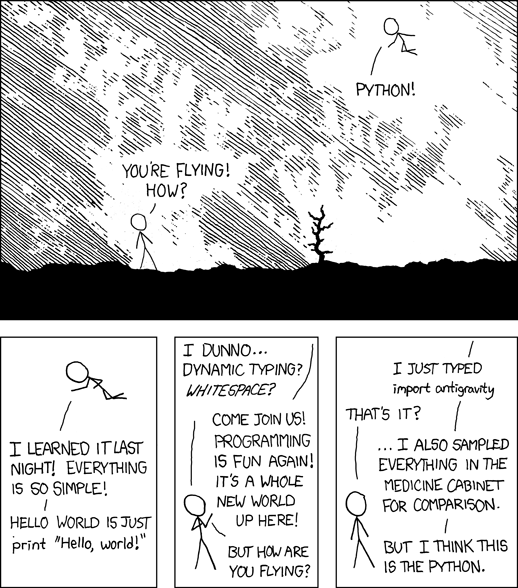
\includegraphics[width=.4\linewidth]{./gfx/xkcd-python}
\captionof{figure}
	[Antigravity in Python]
	{Antigravity in Python. Quelle: \url{https://xkcd.com/353/}}
\end{center}

Diese Euphorie soll nicht darüber hinweg täuschen, dass wir uns der schwierigen Aufgabe stellen, einem Computer unseren Willen abzuverlangen. Aber ähnlich wie Randall Munroe und ich werden Sie beim Erlernen dieser Fähigkeit mit Python schnell Erfolgserlebnisse haben und sicher Spaß daran finden.

Dieses Script soll Sie in der Vorlesung \emph{\myTitle} im \currentPeriod begleiten. Alle wichtigen Kursinhalte werden hier behandelt und anhand von Beispielen verdeutlicht. Es versteht sich von selbst, dass ein optimaler Lernerfolg nur bei Besuch der Vorlesung gegeben ist. Vorkenntnisse in anderen Programmiersprachen sind zur Arbeit mit diesem Script nicht notwendig.

Hier wird von einer Linux-Arbeits\-umgebung ausgegangen und minimale Grundkenntnisse dieser Arbeits\-umgebung vorausgesetzt (Starten einer Kommandozeilen-Umgebung, Wechsel des Arbeitsverzeichnisses, Aufrufen von Programmen aus der Kommandozeile, Übergabe von Parametern an Programme). Die DozentInnen des Kurses können bei Bedarf erklären, wie die Arbeitsumgebung bedient wird.

Dieses Dokument ist keine vollständige Referenz der Sprache Python. Hier sollen nur die Grundlagen des Programmierens in Python vermittelt werden. Als Standard-Nachschlagewerk empfehle ich die offizielle Dokumentation\url{https://docs.python.org/3/} (englisch). Zum einen finden Sie dort ausführliche und vollständige Erklärungen zu allen Themen, die Ihnen bei der Arbeit mit \emph{Python} begegnen können. Zum anderen haben Sie sicherlich Freude an den vielen Anspielungen auf die Sketche der Britischen Anarcho-Komiker \emph{Monty Python}\footnote{\emph{Das Leben des Brian} und \emph{Die Ritter der Kokosnuß}\footnotemark \;
sollten sie unbedingt sehen!}, nach denen die Sprache benannt ist.
\footnotetext{Ja, die Filme sind so alt, dass man damals \emph{Kokosnuß} noch mit scharfem ß schrieb.} 

Dieses Script wurde nach bestem Wissen und Gewissen zusammengestellt; Code-Beispiele wurden auf wenigstens einer Maschine getestet. Dennoch können menschliche Fehler nicht ausgeschlossen werden. Wem Unstimmigkeiten auffallen oder wer Vorschläge und Anregungen zu diesem Text einbringen will, möge mir dies sehr gerne mitteilen. Ich bin erreichbar unter meiner Email-Adresse:\\ \url{stefan.hartinger@stud.uni-regensburg.de}.
\begin{flushright}
\myName, \myVersionTime
\end{flushright}
		\blankpage
		\tableofcontents

		\clearpage
	}
	
	\setcounter{page}{1}

%	\chapter{Die ersten Schritte}
\epigraph{
	A little girl goes into a pet show and asks for a wabbit. The shop keeper looks down at her, smiles
	and says:\newline
	\enquote{Would you like a lovely fluffy little white rabbit, or a cutesy wootesly little brown rabbit?}\newline
	\enquote{Actually}, says the little girl, \enquote{I don't think my python would notice.}
}{Nick Leaton}

In diesem Abschnitt wollen wir unsere Arbeitsumgebung kennen lernen. Zu diesem Zweck werden wir ein sogenanntes \emph{Hello World} schreiben, \ie ein Programm, das lediglich den Text \texttt{Hello World!} auf dem Bildschirm ausgibt. Im Weiteren werden wir Python dazu benutzen, einfache Rechnungen umzusetzen.



\section{Der Kommandozeilen-Interpreter} \label{sec:Interpreter}
Wenn Sie eine \emph{Kommandozeilen-Umgebung} starten, können Sie Textkommandos an das Betriebssystem senden. Überwiegend handelt es sich dabei um die Anweisung, andere Programme auszuführen. Die Anweisung \texttt{python3}\footnote{Die Programmiersprache Python wurde seit ihrer Veröffentlichung im Jahre 1991 beständig weiterentwickelt. Manche Konzepte mussten komplett überarbeitet werden, so dass die einzelnen Versionen der Sprache nicht zwingend kompatibel miteinander sind. Wir arbeiten in der derzeit aktuellen Version 3.8. Auf einem Rechner können mehrere Python-Interpreter nebeneinander installiert sein. Daher müssen wir beim Aufruf die Versionsnummer 3 mit nennen.} ist ein solcher Befehl. Tippen Sie dies ein und drücken Sie \texttt{[ENTER]} um den Python-Interpreter zu starten.

Sie werden nun einen kurzen Versionstext sehen und hinter drei Pfeilen (\texttt{>{}>{}>}) einen blinkenden Cursor. Obwohl Sie noch immer dasselbe Fenster angezeigt bekommen, sind sie nun in der \emph{Interpreter-Umgebung}. Die Befehle, die Sie hier eingeben können, gehören zum Sprachumfang von Python!


\subsection{Hello World}
Ein solcher Befehl ist \inPy{print}. Er dient dazu, Informationen auf dem Bildschirm auszudrucken -- also genau das, was wir für unser Hello-World-Programm brauchen. Natürlich muss dazu auch angegeben werden, \emph{was} gedruckt werden soll. Wir müssen also einen Text \emph{als Argument übergeben}. Dies tun wir, indem wir den Text in Klammern () und Anführungszeichen \texttt{''''} einrahmen. Die Klammern dienen dazu, klar zu machen, was Argument ist, und was zum restlichen Code gehört. Die Anführungszeichen brauchen wir, um Text, der buchstäblich zu behandeln ist, von anderem Code abzutrennen. (Stellen Sie sich vor, sie wollten den Text \texttt{print} auf dem Bildschirm ausgeben. Der Computer versteht ohne Anführungszeichen den Unterschied zwischen dem Text \texttt{print} und dem Befehl \inPy{print} nicht. Vielleicht verstehen Sie nun den Anfang des Vorworts.) Geben Sie also ein:

\begin{center}
	\inPy{print("Hello World!")}
\end{center}

Der Interpreter reagiert prompt, und auf dem Bildschirm finden Sie exakt das, was Sie erwarten: Die Zeile \texttt{Hello World!}.

Nach den letzten Schritten sollten Sie also folgendes auf dem Bildschirm sehen:
\begin{cmdbox}[Starten des Python-Interpreters und Hello-World]
\begin{minted}{text}
blue-chameleon@blue-chameleon:~$ python3
Python 3.8.2 (default, Apr 27 2020, 15:53:34) 
[GCC 9.3.0] on linux
Type "help", "copyright", "credits" or "license" for more information.
>>> print("hello world!")
hello world!
\end{minted}
%$
\end{cmdbox}

Sollten Sie sich vertippen, wird ihnen dies in Form einer (anfangs etwas kryptischen) Fehlermeldung mitgeteilt:
\begin{cmdbox}[Eingabe mit Fehlern]
\begin{minted}{text}
>>> pirnt("hello world!")
Traceback (most recent call last):
  File "<stdin>", line 1, in <module>
NameError: name 'pirnt' is not defined
\end{minted}
\end{cmdbox}
Die letzte Zeile dieser Fehlermeldung teilt Ihnen mit, dass der Befehl \texttt{pirnt} nicht existiert. Sie werden diese Fehlermeldung sehr häufig bei Tippfehlern sehen, wie dies in diesem Beispiel der Fall war. Da Programme zum Teil sehr lang werden können, unterstützt Sie der Interpreter beim Debuggen, indem in der vorletzten Zeile der Ausgabe die Stelle genannt wird, an der die fehlerhafte Eingabe stattfand: \texttt{line 1} sagt, dass die erste Zeile dieses Codes fehlerhaft war.

Vergessen wir beispielsweise, die Anführungszeichen abzuschließen, erhalten wir eine ähnliche Fehlermeldung:

\begin{cmdbox}[Eingabe mit Fehlern]
\begin{minted}{text}
>>> print("hello world)
  File "<stdin>", line 1
    print("hello world)
                      ^
SyntaxError: EOL while scanning string literal
\end{minted}
\end{cmdbox}
\texttt{EOL} steht für \emph{end of line}: Bevor der \emph{string literal} (also unser Text) durch ein abschließendes Anführungszeichen beendet wurde, endete die Zeile.

Ein interessantes Verhalten erzielen Sie, wenn Sie die abschließende Klammer vergessen: Argumente in Python dürfen sich über mehrere Zeilen erstrecken. Anstatt eine Fehlermeldung zu zeigen, wird der Interpreter Sie über drei Punkte (\texttt{...}) auffordern, die Zeile fortzusetzen. Wenn Sie hier die Klammer nachträglich schließen, erhalten Sie die erwartete Ausgabe:
\begin{cmdbox}[Eingabe über mehrere Zeilen]
\begin{minted}{text}
>>> print("hello world"
... )
hello world
\end{minted}
\end{cmdbox}

Mit dem Befehl
\begin{center}
	\inPy{quit()}
\end{center}
beenden Sie den Kommandozeilen-Interpreter wieder; sie sind nun wieder in der Umgebung Ihres Betriebssystems, wo Sie also \emph{keine} Python-Befehle mehr eingeben können.



\section{Script-Dateien} \label{sec:Scripts}
Mit dem letzten Abschnitt haben Sie den ersten Python-Befehl \inPy{print} kennen gelernt! In den Kommandozeilen-Interpreter eingegeben bewirkt er eine direkte Ausgabe auf dem Bildschirm. Sie werden sehr bald weitaus komplexere Programme schreiben, für die es umständlich wäre, sie Zeile für Zeile für jede Ausführung neu einzugeben.

Stattdessen können Sie ein \emph{Textdokument} anlegen, in dem Sie alle Anweisungen nacheinander eingeben und speichern, und den Interpreter anschließend dazu auffordern, diese Datei zu lesen und den Code darin auszuführen. Wichtig hierbei ist, dass es sich wirklich um eine \emph{reine Textdatei} handelt, dass also keine Formatierungen oder sonstigen Inhalte enthält, die über den reinen Code hinaus gehen. Verwenden Sie also zum Schreiben von Code \emph{nicht} Programme wie Word, LibreOffice o.\,ä., sondern Code/Text-Editoren. Ich empfehle:
\begin{itemize}
\item für Linux
	\begin{itemize}
	\item kate (KDE-Editor): auf die Arbeit mit vielen Programmiersprachen ausgelegt, sehr lightweight
	\item gedit: oft vorinstalliert, minimale Features aber alles notwendige gegeben
	\item geany: auf größere Projekte ausgelegt, aber immer noch hinreichend Ressourcen schonend
	\end{itemize}
\item für Windows
	\begin{itemize}
	\item Notepad++: Bietet alle Funktionalitäten, die das Programmieren angenehm machen, 
		ohne dabei zu viele Systemressourcen zu verbrauchen.\\
		Siehe \url{https://notepad-plus-plus.org/}
	\item Notepad: Immer vorinstalliert. Die Arbeit mit diesem Programm ist oft mühselig, da Features
		wie Syntax Highlighting oder Automatische Einrückung nicht gegeben sind; dafür muss nichts
		installiert werden
	\end{itemize}
\end{itemize}

In diesen (und etwa einer Million weiteren) Editoren können Sie Code verfassen und als \texttt{*.py}-Datei abspeichern. Aus der Kommandozeile können Sie diesen Code an den Interpreter weitergeben, indem Sie eingeben:
\begin{center}
\texttt{python3 [myCode].py}
\end{center}
Wobei \texttt{[myCode]} selbstverständlich durch den von Ihnen vergebenen Dateinamen ersetzt werden muss.


\subsection{Beispiel}
Schreiben Sie den folgenden Code in eine Textdatei, und speichern Sie diese als \texttt{HelloWorld.py} ab. (Achten Sie auch auf Groß/Kleinschreibung).
\begin{codebox}[Datei \texttt{HelloWorld.py}]
\begin{minted}[linenos]{python3}
print("Hello World!")
\end{minted}
\end{codebox}

Starten Sie eine Kommandozeilen-Umgebung, und wechseln in dieser in das Verzeichnis, unter dem Sie die Datei abgespeichert haben\footnote{Stichwort \texttt{cd}. Falls Sie nicht wissen, wie das geht, sprechen Sie bitte Ihre Dozenten an.}. In diesem Fall sei der Code unter \texttt{\textasciitilde/Codes} abgelegt. Zum Ausführen dieses Codes geben Sie also ein:

\begin{cmdbox}[Starten des Python-Interpreters und Hello-World]
\begin{minted}{text}
blue-chameleon@blue-chameleon:~$ cd Codes/
blue-chameleon@blue-chameleon:~/Codes$ python3 HelloWorld.py 
Hello World!
\end{minted}
\end{cmdbox}



\section{IDEs}
Neben der Arbeit mit Texteditoren, die vom Interpreter abgegrenzt stehen, existieren auch IDEs, also \emph{Integrated Development Environments}. Es handelt sich dabei um Programme, die eine direkte Anbindung an den Interpreter haben und somit Code-Schreiben und Ausführen im selben Fenster erlauben.

Viele empfinden es als bequemer, mit IDEs zu arbeiten. Diese Programme sind oft aber auch etwas aufwändiger gebaut, und brauchen länger, bis sie geladen sind. Experimentieren Sie hier selbst, welcher Modus Ihnen am besten zusagt; für den Kurs sind beide Wege -- Text-Editor und IDE -- gangbare Wege.

Ich empfehle die IDE spyder3. Linux-User können diese einfach aus dem Paketverwaltungssystem heraus installieren; Windows-User mögen von \url{https://www.spyder-ide.org/} die Installationspakete herunterladen.

\begin{figure}
	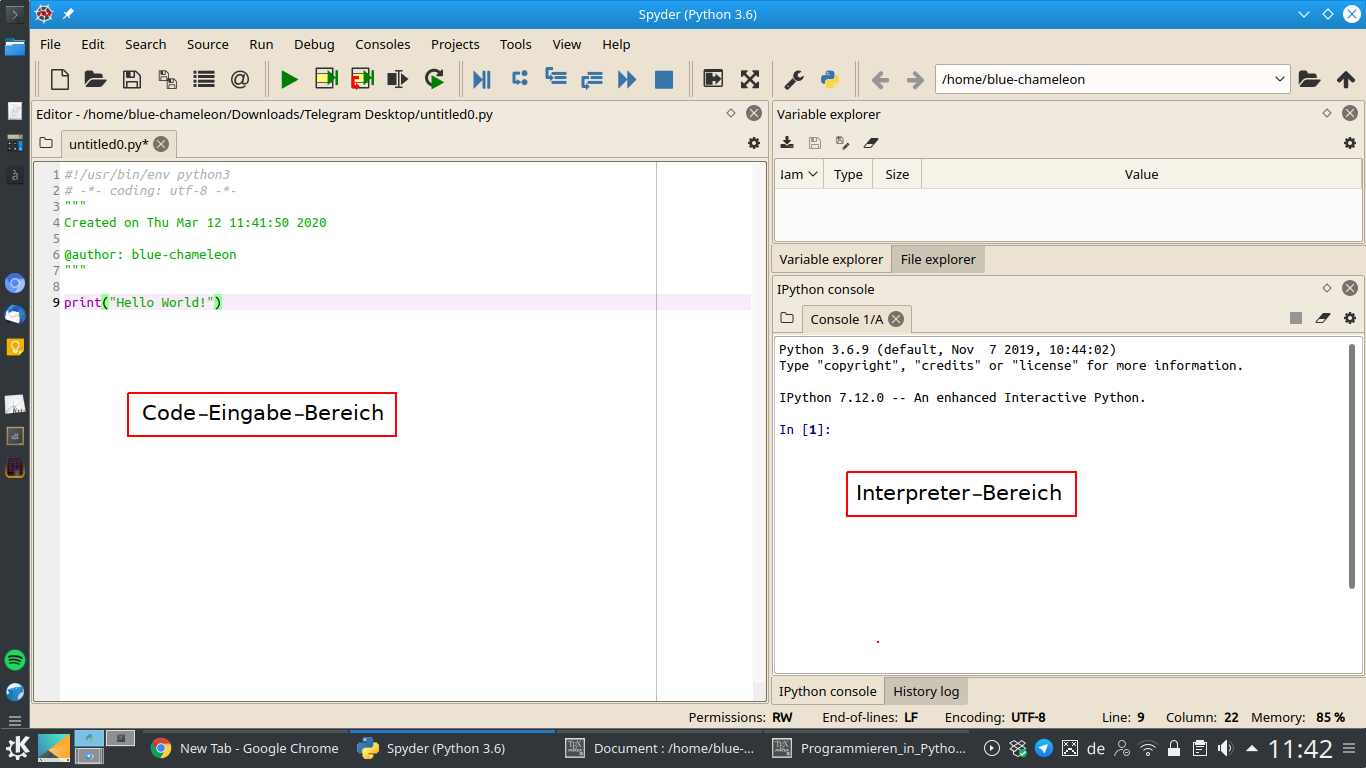
\includegraphics[width=\linewidth]{./gfx/Spyder}
	\caption{Die IDE Spyder} \label{gfx:Spyder}
\end{figure}

In Abbildung \ref{gfx:Spyder} sehen Sie die Arbeitsumgebung des Programms Spyder. Insbesondere finden Sie links einen größeren Bereich, in dem sie komplexere Codes schreiben können, wie schon in Abschnitt \ref{sec:Scripts} angedeutet. In der rechten Fensterhälfte sehen Sie den Interpreter-Bereich, in den Sie direkt Python-Kommandos eingeben können. Genauso, wie in Abschnitt \ref{sec:Interpreter} gezeigt, werden die Befehle, die Sie hier eintippen, sofort ausgeführt.



\section{Rechnen}
Wie erwähnt können wir Python dazu benutzen, einfache Berechnungen ausführen zu lassen. Dazu tippen wir diese einfach direkt in die Interpreter-Umgebung ein:
\begin{cmdbox}[Python als \enquote{Taschenrechner}]
\begin{minted}{text}
>>> 1 + 2
3
\end{minted}
\end{cmdbox}

Diese Rechnungen dürfen aus beliebig vielen Operationen bestehen, halten sich an die Regel \enquote{Punkt vor Strich} und können auch Klammern enthalten:
\begin{cmdbox}[Python als \enquote{Taschenrechner}]
\begin{minted}{text}
>>> ((1 - 5) * 3) / (4 + 1) ** 2
-0.48
\end{minted}
\end{cmdbox}

Dabei werden folgende Zeichen als Operatoren verstanden:
\begin{table}[h!]
\newcolumntype{O}{>{\centering\ttfamily\arraybackslash}m{.2 \textwidth}}
\newcolumntype{F}{>{\centering         \arraybackslash}m{.6 \textwidth}}
\newcolumntype{X}{>{\centering\ttfamily\arraybackslash}m{.2 \textwidth}}

\rowcolors{1}{white}{tabhighlight}
\begin{tabularx}
	{\linewidth}
	{OFX}
	\toprule[1.5pt]

	\normalfont	\bfseries Zeichen &
				\bfseries Funktion &
				\bfseries Beispiel
	\tabcrlf
	+  & Addition					& 1 + 2 = 3 \tabcrlf
	-  & Subtraktion					& 5 - 7 = -2 \tabcrlf
	*  & Multiplikation				& 2 * 4 = 8 \tabcrlf
	/  & Division					& 7 / 5 = 1.4 \tabcrlf
	// & Ganzzahl-Division			& 7 // 5 = 1 \tabcrlf
	\% & Modulo (Rest der Division)	& 7 \% 5 = 2 \tabcrlf
	** & Potenzierung				& 3 ** 2 = 9 \\
	
	\bottomrule[1.5pt]	
\end{tabularx}
\caption{Rechenoperatoren in python3}
\end{table}

Auch das Rechnen mit \emph{komplexen Zahlen} ist möglich. Als imaginäre Einheit wird das Zeichen \inPy{j} verwendet:
\begin{cmdbox}[Komplexe Zahlen]
\begin{minted}{text}
>>> (1j)**2
(-1+0j)
\end{minted}
\end{cmdbox}
Wie Sie sehen, wird das Ergebnis von Rechnungen mit komplexen Zahlen als komplexe Zahl ausgegeben, selbst wenn die Zahl rein reell ist. Mehr dazu im Abschnitt \ref{sub:datatypes}.


\subsection{Variablen}
Die Ergebnisse einer Rechnung können in \emph{Variablen} gespeichert werden. Es handelt sich hierbei um Speicherstellen, denen Sie einen mehr oder minder beliebigen Namen geben können:
\begin{cmdbox}[Variable für Zwischenergebnisse]
\begin{minted}{text}
>>> x = 3 + 7
>>> x ** 2
100
\end{minted}
\end{cmdbox}

Variablen können einzelne Buchstaben sein, dürfen aber auch ganze Worte zum Namen haben. Im Variablennamen dürfen auch der Unterstrich (\_) und die Ziffern 0-9 vorkommen; jedoch muss das erste Zeichen ein Buchstabe sein. Python ist \emph{case sensitive}, \ie zwischen Groß- und Kleinschreibung wird unterschieden.

\begin{table}[h!]
\newcolumntype{O}{>{\centering\ttfamily\arraybackslash}m{.3 \textwidth}}
\newcolumntype{F}{>{\centering         \arraybackslash}m{.3 \textwidth}}
\newcolumntype{X}{>{\centering         \arraybackslash}m{.5 \textwidth}}

\rowcolors{1}{white}{tabhighlight}
\begin{tabularx}
	{\linewidth}
	{OFX}
	\toprule[1.5pt]

	\normalfont	\bfseries Name &
				\bfseries Erlaubt &
				\bfseries Begründung
	\tabcrlf
	x  						& ja 	& \tabcrlf
	counter					& ja 	& \tabcrlf
	CounTer					& ja 	& \tabcrlf
	number\_of\_elements		& ja 	& \tabcrlf
	list4					& ja 	& \tabcrlf
	5th\_list 				& nein	& Ziffer als erstes Zeichen \tabcrlf
	list 4 					& nein	& Leerzeichen \tabcrlf
	Best\_List\_Ever!		& nein	& Rufezeichen \tabcrlf
	print					& Problematisch	& überschreibt den Befehl print\\
	
	\bottomrule[1.5pt]	
\end{tabularx}
\caption{Beispiele für Variablen in python3}
\end{table}

\begin{hintbox}[Sprechende Variablennamen]
Ihre Programme werden sehr bald einige Komplexität annehmen. Sie sollten daher Variablen so benennen, dass auf den ersten Blick erkennbar wird, welche Art Information gespeichert wird. Der Name \inPy{ListLength} ist in jedem Fall dem Namen \inPy{l} vorzuziehen.
\end{hintbox}
%
\begin{hintbox}[Schlüsselworte]
Die Liste oben nennt das Symbol \inPy{print} als erlaubten, aber problematischen Namen. Tatsächlich können Sie in Python die Sprachelemente umdefinieren, und so etwa \inPy{print} als Variable benutzen oder eine andere Routine unter diesem Namen aufrufen. Im Sinne von Lesbarkeit und Kompatiblität mit anderen Programmen sollten Sie hiervon aber Abstand nehmen! Wenn Sie \inPy{print} überschreiben, können Sie zunächst nichts mehr auf dem Bildschirm ausgeben.

Da Sie gerade erst beginnen, die Sprache Python zu erlernen, können Sie natürlich noch nicht alle Symbole kennen, die bereits vergeben sind. Wenn Sie einen Editor mit Syntax-Highlighting verwenden, können Sie aber \idR diese farblichen Markierungen zur Hilfe nehmen: Wenn der Editor ihr Symbol wie einen Befehl markiert, sollten Sie es umbenennen. Wird keine besondere Farbe zugewiesen, so ist der Name vermutlich noch frei. Einige Schlüsselworte sind besonders geschützt, und können nicht überschrieben werden. Sie erhalten die Fehlermeldung \texttt{SyntaxError: invalid syntax}, falls Sie versuchen, ein solches Schlüsselwort als Variablenname zu verwenden.
\end{hintbox}

\begin{hintbox}[Unterstriche in Variablennamen]
Variablennamen dürfen prinzipiell an jeder Stelle Unterstriche enthalten, auch als erstes Zeichen. Es ist aber Konvention, dies nur in bestimmten Situationen zu tun, auf die ich an gegebener Stelle erst eingehen werde. Vermeiden Sie daher vorerst Namen wie \inPy{_var}.
\end{hintbox}

\begin{hintbox}[Non-ASCII-Variablennamen (Umlaute{,} Sonderzeichen{,} \ldots)]
Python 3 erlaubt es prinzipiell, Variablennamen aus dem UTF-8-Zeichenvorrat zu wählen. Das bedeutet, dass neben den lateinischen Klein- und Großbuchstaben (a-z, A-Z) auch Umlaute, Zeichen mit Akzenten, griechische, japanische, \ldots Zeichen für Variablennamen erlaubt sind. Dies führt aber schnell zu Kompatibilitätsproblemen. Neben den offensichtlichen Problemen -- Kollegen in anderen Ländern könnten die Schriftzeichen, die zur Bedienung Ihres Codes nötig sind, nicht eingeben können -- ist manchmal schon das Versenden und Ausführen von Code auf einem anderen Rechner in derselben Arbeitsgruppe schwierig.

Während Python also Variablennamen wie \inPy{äußerstWichtig} durchaus erlaubt, sollten Sie also dennoch nur auf den englischen Zeichenvorrat zurückgreifen, und eine Variable beispielsweise \inPy{exceptionallyImportant} benennen.
\end{hintbox}

Variablen können aktualisiert (\ie überschrieben werden). Dies kann auch mit Bezug auf den alten Wert derselben Variable geschehen:
\begin{cmdbox}[Variable für Zwischenergebnisse]
\begin{minted}{text}
>>> x = 1
>>> x
1
>>> x = 2
>>> x
2
>>> x = x + 1
>>> x
3
\end{minted}
\end{cmdbox}

\begin{warnbox}[Python ist kein Gleichungslöser]
Für mathematisch denkende KursteilnehmerInnen mag die Zeile \inPy{x = x + 1} unsinnig wirken. Offensichtlich gibt es keine Zahl \inPy{x}, die diese Gleichung erfüllt. In Python beschreiben wir auf diese Art aber auch keine Gleichung, sondern einen Arbeitsauftrag: Speichere in der Variable \inPy{x} den Wert der Summe des aktuellen Werts von \inPy{x} plus 1!

Denken Sie an das Vorwort bei der Arbeit mit Computern: Maschinen verstehen komplexe Aufgaben wie das Lösen eines Gleichungssystems nicht.
\end{warnbox}

\begin{hintbox}[Shorthands, parbox=True]
Das Aktualisieren eines Werts unter Bezug auf den alten Wert ist ein häufiger Arbeitsschritt beim Programmieren. Daher wurden Abkürzungen (Shorthands) eingeführt. So steht zum Beispiel der Ausdruck
\vspace{-6pt}
\begin{center}
	\inPy{x += 1}
\end{center}
\vspace{-6pt}
für den Code
\vspace{-6pt}
\begin{center}
	\inPy{x = x + 1}
\end{center}
Ähnlich sind auch \inPy{x -= y}, \inPy{x *= y}, usw. erlaubt.
\end{hintbox}

Die Werte von Variablen können in einem Schritt getauscht werden, indem wir ein Komma zur Hilfe nehmen:
\begin{cmdbox}[Variable für Zwischenergebnisse]
\begin{minted}{text}
>>> x = 1
>>> y = 2
>>> x, y = y, x
>>> x
2
>>> y
1
\end{minted}
\end{cmdbox}
Ein \emph{Dreieckstausch} (\ie die Zuhilfe-Nahme einer dritten Variable) ist nicht nötig. (Intern führt Python einen Dreieckstausch aus; dies wird aber automatisch für Sie erledigt, ohne weiteres zutun Ihrerseits).


\subsection{Datentypen} \label{sub:datatypes}
In diesem Abschnitt arbeiten wir mit Zahlen. Für Sie als Mensch ist eine Zahl eindeutig durch ihren Wert bestimmt: 1 = 1.0 = 1 + 0j = eins. Ein Computer \enquote{kennt} aber zunächst keine Werte, sondern nur binäre Information. Einer Folge von Einsen und Nullen kann nicht angesehen werden, ob diese jetzt eine ganze Zahl, eine komplexe Zahl, einen Teil eines Bildes oder eine Anweisung eines Computerprogramms darstellen. Daher wird jeder Information ein \emph{Datentyp} zugeordnet, also eine Anweisung, wie die Folge von Einsen und Nullen zu interpretieren ist.

Vorerst beschäftigen wir uns mit vier Datentypen:
\begin{itemize}
\item \inPy{int} -- Ganzzahlen, also \inPy{0}, \inPy{1}, \inPy{2}, \inPy{3}, 
		\ldots, sowie negative Ganzzahlen
\item \inPy{float} -- Fließkommazahlen, also \inPy{3.14} oder \inPy{1.0}. (Beachten Sie: als
		Dezimaltrennzeichen verwenden wir einen \emph{Punkt}, kein Komma.)
\item \inPy{complex} -- Komplexe Zahlen, also \inPy{(1+2.7j)}
\item \inPy{str} -- Strings, also Zeichenketten wie \inPy{"Hallo Welt"}
\end{itemize}

Der Datentyp eines Werts wird bei seiner \enquote{Berechnung} festgelegt und zusammen mit der Variablen gespeichert, über die der Wert Verfügbar gehalten wird. Dabei gilt die Grundregel, dass keine Information verloren gehen darf. Bei der Addition einer Ganzzahl (\inPy{int}) und einer Fließkommazahl (\inPy{float}) darf beispielsweise die Information über die Nachkomma-Anteil nicht verloren gehen (selbst, wenn dieser \inPy{.0} ist). Betrachten Sie hierzu folgendes Beispiel:

\begin{cmdbox}[Datentypen bei Addition]
\begin{minted}{text}
>>> 1 + 1
2
>>> 1.0 + 1
2.0
>>> 1 + 1.0
2.0
>>> 1.0 + 1.0
2.0
\end{minted}
\end{cmdbox}

In der ersten Zeile (\inPy{1 + 1}) sind nur Ganzzahlen beteiligt. Somit ist das Ergebnis auch eine Ganzzahl, und wird folgerichtig als solche (\ie ohne Nachkommastelle) ausgegeben. In allen anderen Fällen ist immer mindestens eine Fließkommazahl beteiligt; das Ergebnis ist daher immer \inPy{2.0} (nicht nur \inPy{2}).

Bei der Division wird immer eine Fließkommazahl berechnet, egal ob die Argumente vom Typ \inPy{int} oder \inPy{float} sind.

Ähnlich verhält es sich bei komplexen Zahlen: Sobald eine komplexe Zahl an der Rechnung beteiligt ist, wird auch das Ergebnis vom Typ \inPy{complex} sein. Da \inPy{complex}-Werte auch Nachkomma-Werte speichern können, übertrifft diese Regel die bzgl. \inPy{float}s.

Wenn Sie sich nicht sicher sind, welchen Datentyp eine Variable hat, können Sie den Befehl
\begin{center}
	\inPy{type(Ausdruck)}
\end{center}
benutzen. Dabei steht \inPy{Ausdruck} für eine Variable, eine Zahl oder eine komplette Rechnung.

\begin{cmdbox}[Beispiele zu \texttt{type} (1)]
\begin{minted}{text}
>>> type(1)
<class 'int'>
>>> type(1.0)
<class 'float'>
>>> type(1j)
<class 'complex'>
>>> type(1+1.0)
<class 'float'>
>>> a=1j**2
>>> type(a)
<class 'complex'>
>>> a
(-1+0j)
\end{minted}
\end{cmdbox}

Wollen Sie erzwingen, dass das Ergebnis in einen bestimmten Typ umgewandelt wird, so können Sie den Datentyp vor einen Ausdruck setzen, und diesen einklammern:
\begin{center}
	\inPy{Datentyp(Ausdruck)}
\end{center}

Dabei können Informationen verloren gehen:
\begin{cmdbox}[Beispiele zu \texttt{type} (2)]
\begin{minted}{text}
>>> a = int(1 + 1.9)
>>> type(a)
<class 'int'>
>>> a
2
\end{minted}
\end{cmdbox}
in diesem Beispiel etwa wird der Nachkommaanteil abgeschnitten.

Wie bereits erwähnt, sind Strings (Zeichenketten) dadurch erkennbar, dass ihr Inhalt durch doppelte Anführungszeichen (''\ldots'') vom restlichen Code abgegrenzt wird. Alternativ können auch einfache Anführungszeichen ('\ldots') verwendet werden. Dies hat den Zweck, es Programmierern einfach zu machen, Strings zu Erzeugen, in denen auch selbst wieder Anführungszeichen vorkommen.

\begin{cmdbox}[Beispiele zu Strings (1)]
\begin{minted}{text}
>>> 'abc'
'abc'
>>> "abc"
'abc'
>>> "abc'def'ghi"
"abc'def'ghi"
>>> 'abc"def'
'abc"def'
\end{minted}
\end{cmdbox}

Auch mit Strings kann \enquote{gerechnet} werden; hier sind jedoch nur die Addition (\inPy{+}) und die Multiplikation (\inPy{*}) mit Ganzzahlen definiert. Die Addition verkettet zwei Strings; die Multiplikation wiederholt einen String mehrere Male:

\begin{cmdbox}[Beispiele zu Strings (2)]
\begin{minted}{text}
>>> "ab" + 'cd'
'abcd'
>>> 3 * "ab"
'ababab'
>>> 0 * "ab"
''
>>> "ab" + "'c'def"
"ab'c'def"
\end{minted}
\end{cmdbox}

Die Befehle \inPy{int}, \inPy{float}, \inPy{complex} können -- in begrenztem Maße -- auch auf Strings angewandt werden:

\begin{cmdbox}[Konversion von Strings zu Zahlentypen]
\begin{minted}{text}
>>> int("1")
1
>>> int("1.3")
Traceback (most recent call last):
  File "<stdin>", line 1, in <module>
ValueError: invalid literal for int() with base 10: '1.3'
>>> float("1.3")
1.3
>>> float("1,3")
Traceback (most recent call last):
  File "<stdin>", line 1, in <module>
ValueError: could not convert string to float: '1,3'
>>> complex("1j")
1j
>>> int("one")
Traceback (most recent call last):
  File "<stdin>", line 1, in <module>
ValueError: invalid literal for int() with base 10: 'one'
\end{minted}
\end{cmdbox}

Wie Sie sehen, wird die Darstellung als Text in Zahlen zurückverwandelt, sofern das für den gewünschten Zieltyp möglich ist; andernfalls erhalten Sie eine Fehlermeldung.

Machen Sie sich klar: Für den Computer sind Text und Zahlen unterschiedliche Informationen! Eine \emph{semantische} Interpretation ist nicht möglich. Machen Sie sich daher auch klar, was der Unterschied zwischen diesen drei Additionen ist:
\begin{cmdbox}[Strings und \texttt{int}s (1)]
\begin{minted}{text}
>>> x = "1"
>>> y = "2"
>>> x + y
'12'
>>> int(x + y)
12
>>> int(x) + int(y)
3
\end{minted}
\end{cmdbox}

Wir beginnen mit den \emph{String}-Variablen \inPy{x} und \inPy{y}. Die Addition von Strings ist gleichbedeutend mit der Verkettung; daher ist das Ergebnis von \inPy{x + y} auch folgerichtig der \emph{String} \inPy{"12"}.

Der Aufruf von \inPy{int} in \inPy{int(x + y)} erhält als Argument den Wert \texttt{x + y}, also den \emph{String} \inPy{"12"}. Folgerichtig wird die \emph{Zahl} \inPy{12} berechnet.

Im dritten Teilbeispiel \inPy{int(x) + int(y)} dagegen werden separat die Zahlen \inPy{1} und \inPy{2} aus den Variablen \inPy{x} und \inPy{y} berechnet, und diese dann addiert. Entsprechend kann erst hier das Ergebnis die Zahl \inPy{3} sein.

Natürlich können Sie auch beliebige Zahlen in Strings umwandeln; dazu verwenden Sie einfach den Befehl \inPy{str}:

\begin{cmdbox}[Strings und \texttt{int}s (2)]
\begin{minted}{text}
>>> x = 1
>>> y = 2
>>> str(x + y)
'3'
>>> str(x) + str(y)
'12'
\end{minted}
\end{cmdbox}

\begin{hintbox}[Sprechweise: \emph{dynamische Typisierung} und \emph{duck-typing}]
In vielen Programmiersprachen wird der Datentyp von Variablen einmal festgelegt und darf sich dann für das weitere Programm nicht mehr ändern. Python dagegen erlaubt \emph{dynamische Typisierung}: Eine Variable \inPy{x} kann an einer Stelle des Programms Ganzzahlen speichern und an späterer Stelle Strings. Damit einher geht eine gewisse Ambivalenz; es ist nicht zwingend sofort einsichtig, welchen Datentyp ein Ausdruck hat. Der Python-Interpreter versucht dann, den geeignetsten Datentyp zu \enquote{erraten}. Gemäß dem Zitat von James Whitcomb Riley:
\begin{tcolorbox}[title=Zitat]
When I see a bird that walks like a duck and swims like a duck and quacks like a duck, I call that
bird a duck.
\end{tcolorbox}
wird Python daher als \emph{duck typed language} bezeichnet.
\end{hintbox}


\subsection{Ausgabe von Variablen mit \inPy{print}}
Um den in einer Variablen gespeicherten Wert zu erfahren, haben wir bisher in der Interpreter-Umgebung den Namen der Variable eingegeben. In längeren Codes, wie wir sie im Code-Eingabe-Bereich schreiben, funktioniert dies aus technischen Gründen leider nicht. Stattdessen können wir aber den \inPy{print} benutzen. Betrachten Sie das folgende Beispiel:

\begin{codebox}[Beispiel: Ausgabe von Werten mit \texttt{print}]
\begin{minted}[linenos]{python3}
a = 2
b = a * 7.5 + 2
print(a, b, "konstanter Text", a * "x")
\end{minted}
\end{codebox}

\begin{cmdbox}[Ausgabe: Ausgabe von Werten mit \texttt{print}]
2 17.0 konstanter Text xx
\end{cmdbox}

Sie erkennen hieraus, dass Sie der Befehl \inPy{print} die \emph{Werte der Ausdrücke, die als Argumente übergeben werden}, ausgibt. Das bedeutet, dass \inPy{a} eben durch seinen Wert (hier also durch \inPy{2}) ersetzt wird. Ich erinnere Sie nochmals daran, dass dies der Grund ist, warum Strings in Anführungszeichen eingefasst werden müssen -- sonst könnte der Interpreter die Anweisung \emph{drucke den Buchstaben a} und die Anweisung \emph{drucke den Wert der Variablen }\inPy{a} nicht auseinander halten.

Weiter sehen Sie, dass \inPy{print} nicht nur einen einziges Argument verarbeiten kann, sondern auch mit einer ganzen \emph{Parameterliste} zurecht kommt. Die einzelnen Ausdrücke werden durch Kommata gelistet aufgelistet und der Reihe nach ausgewertet, bevor sie auf dem Bildschirm erscheinen. Diese Ausdrücke dürfen einzelne Variablen (\inPy{a}, \inPy{b}), Konstanten (\inPy{3.14}, \inPy{"konstanter Text"}) oder komplette \enquote{Rechnungen} (\inPy{a * "x"}) sein.



\section{Kommentare und mehrzeilige Kommandos}
Wie Sie bald sehen werden, können Codes lang und komplex werden. Es wird Ihnen helfen, schwer erfassbare Abschnitte durch Fließtext-Kommentare zu ergänzen. Solche Kommentare markieren Sie durch ein Raute-Zeichen (\#). Der Interpreter wird alle Zeichen hinter dem Kommentar-Zeichen bis zum Zeilenende ignorieren.

\begin{codebox}[Beispiel: Kommentare]
\begin{minted}[linenos]{python3}
print("Normaler Code, der ausgeführt wird")  # Dies wird nicht mehr ausgeführt
#print("auch dies wird nicht ausgeführt")
\end{minted}
\end{codebox}

Normalerweise enden Python-Anweisungen mit dem Zeilenumbruch. An manchen Stellen kann es Ihren Code übersichtlicher machen, Anweisungen auf mehrere Zeilen zu verteilen. Dass eine Anweisung trotz Zeilenumbruch über das Zeilenende gelesen werden soll, erreichen Sie, indem Sie einen Backslash (\textbackslash) setzen:

\begin{codebox}[Beispiel: Mehrzeilige Anweisungen]
\begin{minted}[linenos]{python3}
x = 1
a = 2 + \
    3 * x + \
    4 * x**2 + \
    7 * x**3
\end{minted}
\end{codebox}


\section{Formatierte Strings}
Wir können Strings erzeugen, in denen die Werte von Variablen als Text dargestellt werden. Zu diesem Zweck haben wir bereits die Funktion \inPy{str} kennengelernt. Wir wissen auch, dass wir Strings durch die Addition verketten können. Ein bequemerer Weg kann über \emph{Format-Strings} erreicht werden:
\begin{codebox}[Syntax: Format-String]
\begin{minted}{python3}
f"normaler Text {Ausdruck} mehr normaler Text {weiterer Ausdruck:Format} ..."
\end{minted}
\end{codebox}

Ein Format-String beginnt also mit einem vorangestellten \inPy{f}, und wird ebenso von doppelten Anführungszeichen \inPy{""} eingeschlossen, wie ein normaler String. Er kann -- muss aber nicht -- beliebig lange Blocks von Text enthalten, die 1:1 in das Endergebnis übernommen werden. Neu gegenüber normalen Strings sind Blöcke der Form \inPy{{Ausdruck}} und \inPy{{Ausdruck : Format}}.

Wie schon zuvor auch steht \inPy{Ausdruck} für eine Variable, eine Zahl oder eine komplette Rechnung. Der Ausdruck wird zuerst \emph{evaluiert} (\enquote{ausgerechnet}), und dann in den String eingebaut. Die \{geschweiften Klammern\} sind nicht Teil des Endprodukts, sondern zeigen dem Interpreter an, dass hier eine Ersetzung gemacht werden muss.

\begin{codebox}[Beispiel: Formatstrings]
\begin{minted}[linenos]{python3}
a = 1
b = 2
s = f"a + b = {a + b}"
print(s)
\end{minted}
\end{codebox}

\begin{cmdbox}[Ausgabe: Formatstrings]
a + b = 3
\end{cmdbox}

Dieser Code ist im Ergebnis gleichwertig zu 
\begin{codebox}[Beispiel: Gleichwertiger Code ohne Formatstrings]
\begin{minted}[linenos]{python3}
a = 1
b = 2
s = "a + b = " + str(a + b)
print(s)
\end{minted}
\end{codebox}

Wenn Sie tatsächlich \{geschweifte Klammern\} im Ergebnis brauchen, so erreichen sie dies, indem Sie im Formatstring ein doppeltes Klammerpaar setzen:
\begin{codebox}[Beispiel: Formatstrings mit Escape-Sequenz]
\begin{minted}[linenos]{python3}
a = 1
b = 2
s = f"{{a + b}} = {{{a + b}}}"
print(s)
\end{minted}
\end{codebox}
\begin{cmdbox}[Ausgabe: Formatstrings mit Escape-Sequenz]
\begin{minted}{text}
{a + b} = {3}
\end{minted}
\end{cmdbox}

Im Syntax-Kasten wurde bereits angedeutet, dass abgetrennt durch einen Doppelpunkt noch weitere Angaben zur Formatierung folgen dürfen. In Abschnitt \ref{sec:FormatStringsTable} finden Sie eine Übersicht der unterstützten Formatzeichen. Hier seien nur einige besonders nützliche Beispiele gezeigt:

Die einfachste Formatvorgabe, die sie setzen können, ist eine Zahl. Diese Zahl gibt dann an, wie viele Zeichen zur Darstellung des Ausdrucks verwendet werden sollen. Auf diese Weise können Sie bequem tabellarische Ansichten erstellen:

\begin{codebox}[Beispiel: Formatstrings mit Vorgabe der Zeichenlänge]
\begin{minted}[linenos]{python3}
name1 = "Dusky"
score1 = 9001
name2 = "Joe"
score2 = 666

print(f"{name1:20}: {score1:5}")
print(f"{name2:20}: {score2:5}")
\end{minted}
\end{codebox}
\begin{cmdbox}[Ausgabe: Formatstrings mit Vorgabe der Zeichenlänge]
\begin{minted}{text}
Dusky               :  9001
Joe                 :   666
\end{minted}
\end{cmdbox}

Beachten Sie, dass zwischen dem Doppelpunkt und dem Format \emph{kein} Leerzeichen stehen darf (bzw. dass ein solches eine besondere Funktion hat -- siehe weiter unten)

Wie Sie sehen, werden Strings linksbündig ausgegeben, während Zahlen rechtsbündig formatiert werden. Diese Standard-Einstellung kann durch ein vorangestelltes \inPy{<}, \inPy{>} oder \inPy{^} überschrieben werden:
\begin{codebox}[Beispiel: Formatstrings und Alignment]
\begin{minted}[linenos]{python3}
text  = "sample"
value = 123
print( f"|{text:15}| |{value:15}|" )
print(f"|{text:<15}| |{value:<15}|")
print(f"|{text:>15}| |{value:>15}|")
print(f"|{text:^15}| |{value:^15}|")
\end{minted}
\end{codebox}
\begin{cmdbox}[Ausgabe: Formatstrings mit Vorgabe der Zeichenlänge]
\begin{minted}{text}
|sample         | |            123|
|sample         | |123            |
|         sample| |            123|
|    sample     | |      123      |
\end{minted}
\end{cmdbox}

Ist der Ausdruck zu lang, um mit der vorgegebenen Zeichenzahl gedruckt zu werden, so ignoriert Python die Zeichenzahl und druckt den vollen Text. Durch einen Punkt vor der Zahl bringen Sie Python dazu, stattdesen die Ausgabe abzuschneiden. Dies funktioniert jedoch nur bei Strings, und kann nicht mit den Zeichen \inPy{<}, \inPy{>} oder \inPy{^} kombiniert werden:
\begin{codebox}[Beispiel: Formatstrings und String-Truncation]
\begin{minted}[linenos]{python3}
text = "very long sample text"
print( f"|{text:.4}|" )
\end{minted}
\end{codebox}
\begin{cmdbox}[Ausgabe: Formatstrings und String-Truncation]
\begin{minted}{text}
|very|
\end{minted}
\end{cmdbox}

Natürlich können die Effekte durch Hilfsvariablen dennoch kombiniert werden:
\begin{codebox}[Beispiel: Kombination von Formatierungen über Hilfsvariablen]
\begin{minted}[linenos]{python3}
value = 1234567890
step1 = f"{value}"         # zu String
step2 = f"{step1:.5}"      # Länge beschränken
final = f"|{step2:^10}|"   # zentrieren
print(final)
\end{minted}
\end{codebox}
\begin{cmdbox}[Ausgabe: Formatstrings und String-Truncation]
\begin{minted}{text}
|  12345   |
\end{minted}
\end{cmdbox}

Bei \emph{Zahlen} dient ein vorangestelltes Leerzeichen im Formatstring als Platzhalter für ein eventuelles Vorzeichen. Alternativ kann auch ein Pluszeichen (\inPy{+}) gesetzt werden, um anzudeuten, dass das Vorzeichen \emph{immer} Teil des Ergebnisses sein soll, selbst wenn die Zahl positiv ist:
\begin{codebox}[Beispiel: Formatstrings und Vorzeichen]
\begin{minted}[linenos]{python3}
pos =  10
neg = -10
print(f"|{pos: 15}| |{neg: 15}|")
print(f"|{pos:+15}| |{neg:+15}|")
\end{minted}
\end{codebox}
\begin{cmdbox}[Ausgabe: Formatstrings und Vorzeichen]
\begin{minted}{text}
|             10| |            -10|
|            +10| |            -10|
\end{minted}
\end{cmdbox}

Eine vorangestellte \inPy{0} füllt den zur Verfügung gestellten Platz mit Nullen auf. Dies ist mit Leerzeichen und Pluszeichen kombinierbar: 
\begin{codebox}[Beispiel: Formatstrings und führende Nullen]
\begin{minted}[linenos]{python3}
pos =  10
neg = -10
print(f"|{pos: 015}| |{neg: 015}|")
print(f"|{pos:+015}| |{neg:+015}|")
\end{minted}
\end{codebox}
\begin{cmdbox}[Ausgabe: Formatstrings und führende Nullen]
\begin{minted}{text}
| 00000000000010| |-00000000000010|
|+00000000000010| |-00000000000010|
\end{minted}
\end{cmdbox}

Speziell für Fließkommazahlen gibt es das Zeichen \inPy{f}, das eine Steuerung der Anzeige von Nachkommastellen ermöglicht:
\begin{codebox}[Beispiel: Formatstrings und Fließkommazahlen]
\begin{minted}[linenos]{python3}
num = 1.2
print(f"|{num}|")
print(f"|{num:f}|")
print(f"|{num:6.2f}|")
print(f"|{num:<6.1f}|")
print(f"|{num:06.2f}|")
print(f"|{num:+06.2f}|")
print(f"|{num: 06.2f}|")
\end{minted}
\end{codebox}
\begin{cmdbox}[Ausgabe: Formatstrings und Fließkommazahlen]
\begin{minted}{text}
|1.2|
|1.200000|
|  1.20|
|1.2   |
|001.20|
|+01.20|
| 01.20|
\end{minted}
\end{cmdbox}

Ein einzelnes \inPy{f} stellt die Zahl mit 6 Nachkommastellen dar, und füllt gegebenenfalls mit Nullen auf, falls weniger Dezimalstellen zur Zahl gehören. In der Form \inPy{x.yf} werden insgesamt \inPy{x} Zeichen zur Darstellung der Zahl bereitgestellt (Komma und Vorzeichen mitgezählt). Die Zahl wird mit \inPy{y} Nachkommastellen ausgegeben und gegebenenfalls mit Nullen aufgefüllt. Dies ist kombinierbar mit den Alignment-Zeichen \inPy{<}, \inPy{>} und \inPy{^}. Auch führende Nullen, Leerzeichen oder erzwungenes Vorzeichen funktionieren wie oben beschrieben.

\section{Obfuscated Code}
Sie werden feststellen, dass es zu einer Aufgabe sehr viele \emph{funktionierende} Lösungen gibt. Dass Code funktioniert, reicht uns aber nicht. Code soll auch leicht lesbar und verständlich sein. Bedenken Sie: die Aufgaben, die Sie hier lösen, sind in der Regel kein Selbstzweck, sondern Bausteine für größere Projekte. Wenn die einzelnen Teillösungen schwer zu verstehen sind, werden sie auch umso beschwerlicher als Lösung in andere Probleme einbaubar sein.

Das folgende Beispiel:
\begin{codebox}[Beispiel: Unlesbarer Code]
\begin{minted}[linenos]{python3}
p = lambda x: int(( -13214 * x**11 + 956318 * x**10 - 30516585 * x**9 + 
                     564961485 * x**8 - 6717043212 * x**7 + 53614486464 * x**6 
                    -291627605005 * x**5 + 1074222731065 * x**4 
                    -2606048429424 * x**3 + 3927289106268 * x**2
                    -3265905357360 * x + 1116073728000 ) / 19958400)

print (bytearray(map(p, range(1, 13))).decode())
\end{minted}
\end{codebox}
(Quelle: \url{https://codegolf.stackexchange.com/questions/22533/weirdest-obfuscated-hello-world})
gibt ebenso den Text \texttt{Hello World!} auf dem Bildschirm aus, ist aber (auch für Profis) kaum so zu verstehen. Nehmen Sie sich daher die Hinweise zu Best Pratice zu Herzen, die Ihnen in diesem Script mitgegeben werden.
%	\chapter{Usereingaben und Entscheidungen}
\epigraph{
	We must believe in free will -- we have no choice.
}{Isaac Bashevis Singer}

Im vorigen Kapitel lief unser Programm wie auf Schinen: einmal in Gang gesetzt konnte es nicht von dem vorgeschriebenen Pfad abweichen, das Ergebnis jeder Zeile war vorherbestimmt. In diesem Kapitel wollen wir dies auflockern, indem wir Eingaben des Benutzers annehmen und darauf reagieren.

\section{Usereingaben -- \inPy{input}}
Die Funktion \inPy{input} kann benutzt werden, um Eingaben von der Tastatur zu lesen. Diese werden als String gespeichert und können an eigene Variablen übergeben werden. Optional kann ein \emph{Prompt} angezeigt werden, also ein Text, der den User zur Texteingabe auffordert.

\begin{codebox}[Syntax: \texttt{input}]
\inPy{variable = input(prompt)}
\end{codebox}

In dieser Zeile erkennen Sie ein Schema, das Sie beim Programmieren in Python (und in vielen anderen Sprachen) täglich benutzen werden:

Eine \emph{Funktion} wird aufgerufen, indem ihr Name genannt wird, und in Klammern dahinter eine \emph{Parameterliste} übergeben wird. Dies ist eine durch Kommata getrennte Liste von Werten, wie sie es schon von \inPy{print} kennen. Die Funktion berechnet auf Basis der Argumente in der Parameterliste einen Wert, der wiederum in einer (oder mehreren) Variablen gespeichert oder auch verworfen werdem kann. Neben der Berechnung von Werten können Funktionen auch Nebeneffekte haben, wie etwa die Ausgabe von Text auf dem Bildschirm\footnote{\inPy{print} ist eine Funktion. Sie hat den \enquote{Nebeneffekt}, dass Text ausgegeben wird, und den Rückgabewert \inPy{None}. Mehr dazu später.}.

\begin{codebox}[Beispiel: \texttt{input}]
\begin{minted}[linenos]{python}
inText   = input("Bitte geben Sie eine Zahl ein: ")
inNumber = float(inText)
print("Das Quadrat dieser Zahl ist", inNumber ** 2)
\end{minted}
\end{codebox}

\begin{cmdbox}[Ausgabebeispiel \texttt{input} (1)]
\begin{minted}{text}
Bitte geben Sie eine Zahl ein: 1.5
Das Quadrat dieser Zahl ist 2.25
\end{minted}
\end{cmdbox}


\begin{cmdbox}[Ausgabebeispiel \texttt{input} (2)]
\begin{minted}{text}
Bitte geben Sie eine Zahl ein: eins
Traceback (most recent call last):
  File "inputTest.py", line 2, in <module>
    inNumber = float(inText)
ValueError: could not convert string to float: 'eins'
\end{minted}
\end{cmdbox}

\begin{hintbox}[Tipp: \texttt{input} beim Entwickeln auskommentieren]
Sie werden feststellen, dass es einige Zeit dauert, bis Ihr Code das tut, was Sie möchten. Erst nach einigen Ausführungen des Codes werden Sie alle Fehler gefunden und behoben haben. Wenn Sie für jeden Test neu manuell die Eingaben tätigen müssen, die Sie von Ihrem End-User schließlich verlangen, wird Sie das beim Entwickeln Ihres Codes ausbremsen.

Es bietet sich daher an, \inPy{input}-Zeilen auszukommentieren und stattdessen konstante Werte vorzugeben. Schreiben Sie zum Beispiel:
\begin{codebox}[\texttt{input} auskommentieren]
\begin{minted}[linenos]{python}
inText   = "1.5" # input("Bitte geben Sie eine Zahl ein: ")
inNumber = float(inText)
print("Das Quadrat dieser Zahl ist", inNumber ** 2)
\end{minted}
\end{codebox}
bis Sie sich sicher sind, dass die Codezeilen, die Ihrer Eingabe folgen, tatsächlich Ihre Wünsche erfüllen. Vergessen Sie danach nicht, die Eingabemöglichkeit wiederherzustellen!
\end{hintbox}

\section{Bedingte Codeausführung}
Da wir nun eine Möglichkeit gefunden haben, Eingaben des Users in unseren Programmablauf einzuführen, ist das Ergebnis unseres Programmes nicht mehr schon vor der Ausführung vorherbestimmt. Wir wollen darauf aufbauen, und abhängig von Eingaben Entscheidungen treffen: Einzelne Programmteile sollen nur dann ausgeführt werden, wenn eine \emph{Bedingung} erfüllt ist. Hierzu jedoch zunächst etwas Theorie:

\subsection{Booleans -- Wahrheitswerte}
Mathematischen Ausdrücken können \emph{Wahrheitswerte} zugeordnet werden. Diese Wahrheitswerte sagen aus, ob es sich um eine \enquote{wahre} oder \enquote{falsche} Aussage handelt. Ein Beispiel für einen solchen Ausdruck ist:
\begin{center}
\inPy{1 + 5 * 8 + 1 == 42}
\end{center}
Der Wahrheitswert dieses Ausdrucks ist offensichtlich \emph{wahr} (bzw. \inPy{True}).

Beachten Sie bitte, dass für den \emph{Vergleich} zweier Zahlen das \emph{doppelte Gleichheitszeichen} \inPy{==} verwendet wird. Das einfache Gleichheitszeichen \inPy{=} dient ausschließlich der \emph{Wertzuweisung} an Variablen.

Tabelle \ref{tab:OperatorsComparison} listet weitere Vergleichsoperatoren auf.
\begin{table}[h!]
	\newcolumntype{C}{>{         \centering\arraybackslash} p{.245\linewidth}}
	\newcolumntype{O}{>{\ttfamily\centering\arraybackslash} p{.200\linewidth}}

	\rowcolors{1}{tabhighlight}{white}
\begin{center}
\begin{tabularx}
	{\linewidth}
	{CO|CO}
\toprule[1pt]
	
	\textbf{Vergleich}  & \normalfont \textbf{Zeichen}  &  
	\textbf{Vergleich}  & \normalfont \textbf{Zeichen}
\tabcrlf

	Gleichheit          & ==                   &  Ungleichheit         & != \textrm{oder} <>\\
	Kleiner als         & <                    &  Größer als           & >  \\
	Kleiner oder gleich & <=                   &  Größer oder gleich   & >= \\
	
\bottomrule[1pt]
\end{tabularx}
\end{center}
\caption{Vergleichsoperatoren in Python}\label{tab:OperatorsComparison}
\end{table}

Das Ergebnis eines Vergleichs ist selbst eine Information, die in einer Variablen gespeichert werden kann. Der \emph{Datentyp} eines solches Vergleichs nennt sich \inPy{bool}\footnote{Häufig spricht man auch von \emph{Booleans}, benannt nach dem englischen Mathematiker George Boole.}. Ein solcher Boolean kann nur entweder \inPy{True} oder \inPy{False} sein.

Theoretisch reicht also ein einziges Bit, um die Information \inPy{True/False} zu kodieren. Aus technischen Gründen können jedoch nur Gruppen zu mindestens 8 Bit -- also 1 Byte -- verarbeitet werden. Intern werden \inPy{bool}s daher als \inPy{int}s abgelegt und anders herum \inPy{int}s wie \inPy{bool}s behandelt. Als \inPy{True} gilt dabei jeder Wert, der von \inPy{0} verschieden ist. Sie können Booleans also auch als eine besondere Darstellungsform von \inPy{int}s verstehen.

Mit diesen \emph{Booleans} kann nun auch wieder gerechnet werden. Wenig sinnvoll (aber durchaus möglich) sind die Grundrechenarten (Addition, Subtraktion, ...). Hier zählt \inPy{True} als der \inPy{int 1} während \inPy{False} wie eine \inPy{0} behandelt wird.

Interessanter dagegen sind \emph{logische Verknüpfungen}: Wir können uns eine Gesamtaussage vorstellen, die aus zwei oder mehreren Teilaussagen besteht. So kann die Gesamtaussage \emph{Es ist angenehm warm} dann erfüllt (\inPy{True}) sein, wenn sowohl die Teilaussage \emph{Es ist wärmer als 20°C}, ALS AUCH die Teilaussage \emph{Es ist kälter als 25°C} erfüllt ist. Formal wird dies mit dem \emph{logischen Operator} \inPy{and} ausgedrückt: Nur wenn beide Booleans \inPy{True} sind, ist das Ergebnis von \inPy{and} auch \inPy{True}. Folgendes Beispiel zeigt Ihnen die Anwendung des logischen Operators \inPy{and}:

\begin{codebox}[Beispiel: \texttt{and}]
\begin{minted}[linenos]{python}
temperature = float(input("Bitte geben Sie die aktuelle Temperatur ein: "))

warmEnough = temperature > 20
coldEnough = temperature < 25

pleasantTemperature = warmEnough and coldEnough

print("Die Aussage 'es ist angenehm warm' ist", pleasantTemperature)
\end{minted}
\end{codebox}

\begin{cmdbox}[Ausgabebeispiel \texttt{and}]
\begin{minted}{text}
Bitte geben Sie die aktuelle Temperatur ein: 18
Die Aussage 'es ist angenehm warm' ist False
\end{minted}
\end{cmdbox}

Hier wird \inPy{warmEnough} zu \inPy{False} ausgewertet, während \inPy{coldEnough} den Wert \inPy{True} zugewiesen bekommt. Das Ergebnis von \inPy{False and True} ist nach Boole'scher Algebra wiederum \inPy{False}.

Beachten Sie, dass die \inPy{and}-Zeile auch ohne Hilfsvariablen auskommt:
\begin{center}
	\inPy{pleasantTemperature = (temperature > 20) and (temperature < 25)}
\end{center}
wird genauso ausgewertet wie der oben gezeigte Code.

Neben dem logischen Und (\inPy{and}) gibt es auch das logische Oder (\inPy{or}). Auch hier werden zwei Teilaussagen zu einer Gesamtaussage verknüpft. Beim Oder reicht es aber, wenn nur wenigstens eine Aussage \inPy{True} ist. Ich kann also die Idee \emph{Ich habe keine Probleme, wenn mir jemand zur Seite steht, oder wenn ich keine Hose trage}\footnote{frei nach der Regensburger Philosophin M. Mühlbauer, die mit dem Credo \emph{Keine Hose -- keine Probleme} schon manchen zum Lachen gebracht hat.} im Code ausdrücken als:
\begin{center}
	\inPy{hakunaMatata = somebodyHelpsMe or notWearingPants}
\end{center}
Dabei wird \inPy{hakunaMatata} sowohl \inPy{True}, wenn nur eine der beiden Wahrheitswerte \inPy{somebodyHelpsMe} und \inPy{notWearingPants} gleich \inPy{True} sind, oder auch, wenn \emph{beide} den Wert \inPy{True} haben.

Schließlich existiert noch das logische Nicht (\inPy{not}), das einen Wahrheitswert einfach in sein Gegenteil verkehrt. \inPy{not True} ist \inPy{False}, und \inPy{not False} ist \inPy{True}.

\subsection{\inPy{if}-Blöcke}
Wir können dafür sorgen, dass ein Teil des Codes nur dann ausgeführt wird, wenn ein Wahrheitswert gleich \inPy{True} ist. Dazu verwenden wir das Schlüsselwort \inPy{if}:
\begin{codebox}[Syntax: \texttt{if} (1)]
\begin{minted}{python}
normaler_Code

if Wahrheitswert :
    Anweisungen

normaler_Code
\end{minted}
\end{codebox}

\inPy{Anweisungen} sind beliebige Python-Befehle, wie Sie schon einige kennen gelernt haben, und wie sie noch weitere dazu lernen werden; dasselbe gilt für \inPy{normaler_Code}. Beides können einzeilige Befehle sein oder auch längere Anweisungsblocks.

Während \inPy{normaler_Code} \emph{immer} ausgeführt wird, beachtet der Python-Interpreter die \inPy{Anweisungen} des \inPy{if}-Blocks nur, wenn \inPy{Wahrheitswert} gleich \inPy{True} ist. Zum Block \inPy{Anweisungen} gehört aller Code, der \emph{eingerückt} ist, der also \enquote{nach rechts} verschoben wurde.

\begin{hintbox}[Wie richtig Einrücken?]
Python-Code darf \emph{entweder} durch Leerzeichen \emph{oder} durch Tabulatoren eingerückt werden, nicht jedoch durch eine Mischung aus beiden. Leerzeichen werden empfohlen. Die Anzahl der Leerzeichen je Einrückungsebene kann frei gewählt werden, muss aber über das gesamte Code-Dokument einheitlich gehalten werden. Empfohlen werden vier Leerzeichen pro Ebene.

Viele Code-Editoren setzen automatisch Leerzeichen, wenn die Tabulator-Taste gedrückt wird, und erlauben so ein komfortables Arbeiten. Einige erkennen sogar automatisch Block-Strukturen wie \inPy{if}, und machen automatisch eine Einrückung, wenn nach dem Doppelpunkt Enter gedrückt wird.
\end{hintbox}

Das \inPy{if} kann zu einer \emph{wenn-sonst}-Struktur ausgeweitet werden, indem ein \inPy{else}-Block angefügt wird:
\begin{codebox}[Syntax: \texttt{if} (2)]
\begin{minted}{python}
normaler_Code

if Wahrheitswert :
    Wenn_Anweisungen
else :
    Sonst_Anweisungen
	
normaler_Code
\end{minted}
\end{codebox}

Wie zu erwarten, wird der Block \inPy{Wenn_Anweisungen} nur ausgeführt, wenn \inPy{Wahrheitswert} gleich \inPy{True} ist. Andernfalls (und nur dann!) befolgt der Python-Interpreter den Block \inPy{Sonst_Anweisungen}.

\begin{codebox}[Beispiel: \texttt{if} und \texttt{and}]
\begin{minted}[linenos]{python}
temperature = float(input("Bitte geben Sie die aktuelle Temperatur ein: "))

if (temperature > 20) and (temperature < 25) :
    print("Es ist angenehm warm.")
else :
    print("Es ist entweder zu heiß oder zu kalt.")
\end{minted}
\end{codebox}

Schließlich kann diese Struktur nochmals erweitert werden, um mehrere Bedingungen aneinander zu reihen. Dazu verwenden wir das Schlüsselwort \inPy{elif}, was für \inPy{else if} steht:

\begin{codebox}[Syntax: \texttt{if} (3)]
\begin{minted}{python}
normaler_Code

if Wahrheitswert_1 :
    Anweisungen_1
elif Wahrheitswert_2 :
    Anweisungen_2
elif ...
    ...
else :
    Sonst_Anweisungen
	
normaler_Code
\end{minted}
\end{codebox}

Das \inPy{else} ist hierbei optional. Es dürfen beliebig viele \inPy{elif}-Blöcke aufgereiht werden.

Beachten Sie: von den \inPy{Anweisungen}-Blocks in dieser Struktur wird nur ein einziger ausgeführt! Python prüft zuerst \inPy{Wahrheitswert_1}. Wenn dieser \inPy{True} war, wird \inPy{Anweisungen_1} ausgeführt und danach \emph{sofort} mit \inPy{normaler_Code} fortgesetzt, unabhängig davon, ob \inPy{Wahrheitswert_2} oder andere auch wahr wären. Die Liste der Bedingungen wird von oben nach unten abgearbeitet und nur \emph{der erste erfüllte Bedingungsblock} wird ausgeführt.

Betrachten Sie dazu folgenden Code:
\begin{codebox}[Beispiel: \texttt{elif}]
\begin{minted}[linenos]{python}
temperature = float(input("Bitte geben Sie die aktuelle Temperatur ein: "))

if   temperature < 20 :
    print("Es ist zu kalt.")
elif temperature > 25 :
    print("Es ist zu heiß")
else :
    print("Es ist angenehm warm.")
\end{minted}
\end{codebox}

Das \inPy{and}, das wir zuvor gebraucht haben, ist nun schon in der Anordnung der Bedingungen absorbiert. Die Prüfung \inPy{temperature > 25} wird nur dann überhaupt ausgeführt, wenn \inPy{temperature < 20} bereits \inPy{False} war.

Durchdenken Sie bitte auch dieses \emph{fehlerhafte} Beispiel:
\begin{warnbox}[Fehlerhafter Code: \texttt{elif}, leftupper=7mm]
\begin{minted}[linenos]{python}
i = 23

if   i < 25 :
    print("Diese Zahl ist kleiner als 25.")
elif i > 20 :
    print("Diese Zahl ist größer als 20.")
\end{minted}
\end{warnbox}

Die Zahl \inPy{23} erfüllt zwar beide Bedingungen (\inPy{i < 25} und \inPy{i > 20}). Dennoch wird nur Die Ausgabe \texttt{Diese Zahl ist kleiner als 25.} erfolgen, da die zweite Prüfung (\inPy{i > 20}) nie durchgeführt wird.

\inPy{if}-Blöcke können auch ineinander verschachtelt werden:
\begin{codebox}[Beispiel: Verschachtelte \texttt{if}-Blöcke]
\begin{minted}[linenos]{python}
i = int(input("Bitte geben Sie eine Ganzahl ein: "))

if i % 2 == 0 :
    if   i > 100 :
        print(i, "ist eine große gerade Zahl.")
    elif i <   0 :
        print(i, "ist eine große gerade Zahl.")
    else :
        print(i, "ist eine negative gerade Zahl.")
else :
    print(i "ist ungerade.")
\end{minted}
\end{codebox}

Zuerst findet also die Prüfung statt, ob \inPy{i} gerade ist 
(\inPy{i} \texttt{\%} \inPy{2}).		% \inPy seems to be sensitive to the comment character...
Nur, wenn diese Bedingung erfüllt ist, wird der innere \inPy{if}-Block behandelt. Durch die Einrückungen ist eindeutig festgelegt, zu welcher Bedingung welche Anweisung gehört. Hier beispielsweise ist \emph{der gesamte innere \inPy{if}-Block} der Bedingung 
\inPy{i} \texttt{\%} \inPy{2}		% \inPy seems to be sensitive to the comment character...
untergeordnet.

Das oben gezeigte Beispiel Beispiel: \emph{Verschachtelte \inPy{if}-Blöcke} ist im Ergebnis äquivalent zum folgenden Code:
\begin{warnbox}[Beispiel: Redundanz bei \texttt{if} mit logischen Operatoren, leftupper=7mm]
\begin{minted}[linenos]{python}
i = int(input("Bitte geben Sie eine Ganzahl ein: "))

if   i % 2 == 0 and i > 100 :
    print(i, "ist eine große gerade Zahl.")
elif i % 2 == 0 and i <   0 :
    print(i, "ist eine große gerade Zahl.")
elif i % 2 == 0 :
    print(i, "ist eine negative gerade Zahl.")
else :
    print(i "ist ungerade.")
\end{minted}
\end{warnbox}

Möglicherweise finden Sie diese \enquote{flachere} Form mit weniger Hierarchie-Ebenen leichter zu lesen. Beachten Sie aber auch, dass der Ausdruck
\inPy{i} \texttt{\%} \inPy{2}		% \inPy seems to be sensitive to the comment character...
jetzt ganze dreimal im Code steht. Nicht nur, dass Programme dieser Form langsamer ablaufen (der Ausdruck
\inPy{i} \texttt{\%} \inPy{2}		% \inPy seems to be sensitive to the comment character...
wird tatsächlich bis zu dreimal berechnet!), es ergibt sich hieraus auch eine Fehlerquelle! Stellen Sie sich vor, Sie wollen Ihr Programm zu späterer Zeit anpassen und nun eine andere Bedingung an \inPy{i} stellen. In dieser Form mit redundanten Prüfungen müssen Sie also auch \emph{drei} Codestellen ändern. Häufig aber vergisst man diese Stellen im Falle von redundanten Code.

\begin{warnbox}[Redundanten Code vermeiden]
Sie mögen sich für sehr gewissenhaft halten, und ich glaube Ihnen das gerne. So sicher Sie sich aber auch sind, dass Sie beim Überarbeiten Ihres Codes alle relevanten Stellen überprüfen werden: vermeiden Sie Redundanz! Produktiver Code erreicht schnell Längen von mehreren Tausend Zeilen und wird über Monate hinweg entwickelt. Sie machen sich -- und Ihren Kollegen, die auf Ihrer Arbeit aufbauen wollen -- das Leben unnötig schwer, wenn Sie Code-Teile wiederholen. Hinterfragen Sie sich jedes Mal, wenn Sie einen Copy\&Paste-Schritt machen wollen, ob eine alternative Struktur nicht geeigneter wäre.
\end{warnbox}

Durchdenken Sie zur Verdeutlichung nochmal diese beiden Beispiele:
\begin{tcbraster}[raster columns=2,
                  raster equal height,
                  nobeforeafter,
                  raster column skip=0.5cm]
	\begin{warnbox}[Gültigkeitsprüfung: Reihe von \texttt{if}s, leftupper=7mm]
	\begin{minted}[linenos]{python}
playerCount = int(input(
    "Bitte Spielerzahl eingeben: "
))
      
if playerCount < 2 :
    print("Ungeeignet für", 
          playerCount, 
          "Spieler."
    )
if playerCount > 5) :
    print("Ungeeignet für", 
          playerCount,
          "Spieler."
    )
	\end{minted}
	\end{warnbox}
%
	\begin{codebox}[Gültigkeitsprüfung: logisches Oder]
	\begin{minted}[linenos]{python}
playerCount = int(input(
    "Bitte Spielerzahl eingeben: "
))
      
if  playerCount < 2 or
    playerCount > 5  :
        print("Ungeeignet für",
              playerCount,
              "Spieler."
        )
	\end{minted}
	\end{codebox}
\end{tcbraster}

\begin{hintbox}[Platzhalter für Anweisungen: \texttt{pass}]
Es ist schwierig, die vielen Effekte, die beim Programmieren auftreten, gleichzeitig im Kopf zu behalten. Arbeiten Sie daher kleinschrittig und prüfen Sie nach wenigen neu geschriebenen Code-Zeilen durch Ausführen, ob Ihr Code auch tatsächlich das tut, was Sie erwarten.

Wenn Sie diesen Rat beherzigen, werden Sie \newline
a) schnell funktionierenden Code schreiben, und \newline
b) in folgende Situation kommen:

Block-Strukturen wie \inPy{if} verlangen, dass in jedem Teil-Block Anweisungen stehen. Wenn Sie \inPy{else} schreiben, so \emph{müssen} Sie hierfür auch Anweisungen bereit stellen. Da Sie aber vielleicht erst einen anderen Abschnitt fertig testen wollen, möchten Sie vielleicht den \inPy{else}-Block vorerst leer lassen. In diesem Fall können Sie den Befehl \inPy{pass} benutzen. Dieser macht buchstäblich \emph{nichts}, und wurde genau zu dem Zweck zum Sprachumfang von Python hinzugefügt, um die Schrittweise Entwicklung von Code zu erlauben.
\end{hintbox}

\subsection{Der Ternäre Operator}
Eine häufige Aufgabe beim Programmieren ist die \emph{bedingte Zuweisung} eines Wertes. Abhängig vom Wert eines Ausdrucks soll der Wert einer Variablen gesetzt werden. Sie wissen bereits, dass Sie dies mit einem \inPy{if}-Block erledigen können:
\begin{codebox}[Bedingte Wertzuweisung mit \texttt{if}-Block]
\begin{minted}[linenos]{python}
if Bedingung :
    variable = Wert1
else :
    variable = Wert2
\end{minted}
\end{codebox}

Für diese Aufgabe existiert eine Kurzform des \emph{ternären Operators}\footnote{Operatoren brauchen \emph{Argumente}, aus denen Werte berechnet werden können. Man klassifiziert nach der Zahl der notwendigen Argumente. So gibt es das \emph{unäre} \inPy{not}, das \emph{binäre} \inPy{+} und eben den ternären Operator, der \emph{drei} Argumente braucht.}, die sich schon fast wie englischer Prosa-Text liest:

\begin{codebox}[Bedingte Wertzuweisung mit dem Ternären Operator]
\begin{minted}{python}
variable = Wert1 if Bedingung else Wert2
\end{minted}
\end{codebox}

Sie können diese Ausdrucksform sogar an die Stelle anderer Ausdrücke setzen und beispielsweise an Funktionen als Argument übergeben:

\begin{codebox}[Beispiel: Ternärer Operator als Argument]
\begin{minted}[linenos]{python}
x = float(input("Bitte geben Sie eine Zahl ein: "))
print("Der Betrag von", x, "ist:", x if x > 0 else -x)
\end{minted}
\end{codebox}
%	\chapter{Module Laden}
\epigraph{
	Everything is awesome!
}{Emmet Brickowski}

Die Sprache Python kennt insgesamt nur 33 Schlüsselworte. Aus diesen wenigen Sprachelementen lassen sich erste Algorithmen bauen, die wiederum in komplexeren Routinen eingebaut werden können. Einer der großen Vorteile von Python ist es, dass für die weit meisten Aufgaben, die im Programmierer-Alltag auftauchen, bereits vorgefertigte Routinen zur Verfügung stehen.

Damit Routinen genutzt werden können, müssen diese zunächst im Arbeitsspeicher vorliegen. Kaum ein Programm wird \emph{alle} Routinen benutzen, die in der \emph{Standardbibliothek} der Sprache Python angeboten werden. Um also nicht eine unsinnig große Menge an Speicherplatz zu belegen, bevor auch nur eine einzige Zeile nützlichen Codes ausgeführt wird, können wir selbst bestimmen, welche \emph{Module} geladen werden sollen. Ein Modul ist eine Sammlung von Routinen, die einem gemeinsamen \enquote{Thema} zugeordnet sind (beispielsweise mathematische Funktionen).

\section{Der Befehl \inPy{import}}
Geladen wird ein Modul mit dem Befehl \inPy{import}:
\begin{codebox}[Syntax]
\mint{python3}{import module}
\end{codebox}

Sobald ein Modul geladen ist, können wir die darin zusammen gefassten Funktionen aufrufen. Zwei Module können Funktionen mit gleichem Namen haben. Damit klar ist, welche Funktion wirklich gemeint ist, muss der Modulname beim Funktionsaufruf mit genannt werden:

\begin{codebox}[Syntax]
\mint{python3}{module.function(arguments)}
\end{codebox}

Beispielsweise existieren die Module \inPy{math} und \inPy{cmath}. Beide stellen mathematische Funktionen zur Verfügung; jedoch ist \inPy{math} auf relle Zahlen ausgelegt, \inPy{cmath} dagegen auf komplexe Zahlen. Wir können die Funktionen aus beiden Modulen so benutzen:

\begin{codebox}[Beispiel: Funktionen aus \texttt{math} und \texttt{cmath}]
\begin{minted}[linenos]{python3}
import math
import cmath

print( math. sin( math.pi / 2) )
print( cmath.sin(cmath.pi / 2) )
\end{minted}
\end{codebox}

\begin{cmdbox}[Ausgabe]
1.0 \\
(1+0j)
\end{cmdbox}

Module können ihrerseits wieder aus Unter-Modulen bestehen, so dass sich ein \enquote{Modul-Pfad} ergibt. Ein Beispiel ist die Komponente \inPy{pyplot} aus dem Modul \inPy{matplotlib}, das zur graphischen Darstellung von Daten genutzt werden kann\footnote{Wir werden die Funktionen dieses Moduls ausführlicher in Kapitel \ref{chp:Matplotlib} besprechen. Für hier soll es Ihnen genügen zu wissen, dass dieses Modul existiert.}. Importiert man die \inPy{matplotlib}, so stehen die Funktionen von \inPy{pyplot} unter dem länglichen Präfix \inPy{matplotlib.pyplot} zur Verfügung.

Es ist lästig, für jeden Funktionsaufruf den vollen Präfix \inPy{matplotlib.pyplot} anzugeben. Stattdessen können für diese Modulpfade neue Symbole vergeben werden:

\begin{codebox}[Syntax]
\mint{python3}{import long.module.path as alias}
\end{codebox}

Es ist beispielsweise sehr geläufig, das angesprochene Modul \inPy{matplotlib.pyplot} unter dem \emph{Alias} \inPy{plt} zu laden:
\begin{codebox}[Beispiel: \texttt{import} mit Alias]
\begin{minted}[linenos]{python3}
import matplotlib.pyplot as plt

plt.figure()    # statt matplotlib.pyplot.figure()
\end{minted}
\end{codebox}

Wenn Sie nur einzelne Funktionen eines Moduls benutzen, können Sie auch diese auch alternativ mit \inPy{from} laden:
\begin{codebox}[Syntax]
\mint{python3}{from module import function}
\end{codebox}

Um Namenskollisionen zu umgehen, besteht auch hier die Möglichkeit, ein Alias zu vergeben:
\begin{codebox}[Syntax]
\mint{python3}{from module import function as alias}
\end{codebox}
Dieser Alias darf dann aber keinen Punkt (\texttt{.}) enthalten.

Das obige Beispiel: \emph{Funktionen aus \inPy{math} und \inPy{cmath}} kann also auch folgendermaßen geschrieben werden:
\begin{codebox}[Beispiel: \texttt{from} ... \texttt{import}]
\begin{minted}[linenos]{python3}
from  math import sin
from  math import pi
from cmath import sin as csin

print(  sin(pi / 2) )
print( csin(pi / 2) )
\end{minted}
\end{codebox}

\begin{hintbox}[\texttt{import} oder \texttt{from} ... \texttt{import}?]
Welche der beiden Methoden -- \inPy{import} oder \inPy{from} ... \inPy{import} -- am besten funktioniert, ist letztlich Frage des Geschmacks. Die \inPy{import}-Methode lädt ein Modul als Gesamtpaket, verlangt aber bei jedem Aufruf ein Präfix. Dagegen sind bei \inPy{from} ... \inPy{import} jeweils eigene Zeilen für jede geladene Funktion und Konstante nötig. In jedem Fall sollten Sie konsistent bleiben, \ie nur entweder \inPy{import} oder \inPy{from} ... \inPy{import} benutzen.

In diesem Kurs verwende ich nur die \inPy{import}-Methode. Durch diese ist es leichter, das Verhalten von Funktionen abzuschätzen, da bereits sofort der Kontext mitgeliefert wird. (Eine Funktion aus \inPy{cmath} wird \idR einen Wert vom Typ \inPy{complex} berechnen, während \inPy{math} \idR Werte vom Typ \inPy{float} berechnet. Solche Details können große Auswirkungen haben, und es ist oft gut, im Code direkt daran erinnert zu werden.)
\end{hintbox}

\begin{hintbox}[\texttt{import}-Zeilen am Anfang des Codes]
Funktionen, die mit \inPy{import} (bzw. \inPy{from} ... \inPy{import}) geladen werden, sind \idR für den gesamten Code relevant. Daher sollten die \inPy{import}-Anweisungen auch die ersten Zeilen Ihres Codes darstellen und \emph{nur} dort auftauchen. Auf diese Weise kann ein Leser Ihres Codes sich sofort auf  die verwendeten Methoden einstellen und weiß, wo er oder sie nachlesen kann, für welche Module ihre Aliase stehen.
\end{hintbox}

Die für Python verfügbaren Module haben \idR einen Webauftritt, in der alle Funktionen dokumentiert sind. Die Suchmaschine der Wahl sollte mit dem Begriff \emph{Python [Modulename] Documentation} eine ausführliche Beschreibung zum Funktionsumfang liefern. Auf diese Art finden Sie \ua den Link
\begin{center}
	\url{https://docs.python.org/2/library/math.html}
\end{center}
und damit eine Beschreibung des Python-Moduls \texttt{math}. Stöbern Sie in dieser Auflistung, und gewöhnen Sie sich an die dort verwendete Sprache. Viele komplexe Aufgaben können durch Verwendung eines geeigneten Moduls sehr schnell gelöst werden. Dazu müssen Sie als ProgrammiererIn jedoch die entsprechenden Funktionen identifizeren und sich ihre Benutzung selbst anlesen können. Angesichts der Vielzahl an Aufgaben und verfügbaren Pakete kann kein Kurs erschöpfend auf die verfügaren Funktionen eingehen.

\section{Eigene Module}
Module in Python können auf verschiedene Art umgesetzt werden. In den meisten Fällen handelt es sich aber tatsächlich einfach um normalen Code, wie Sie ihn bereits gesehen haben und im weiteren kennen lernen werden. Das heißt, dass die \texttt{.py}-Dateien, die Sie hier zu schreiben lernen, auch ihrerseits als Module genutzt werden können. Wenn Sie also ihren Code in der Datei \texttt{myModule.py} speichern, so können Sie durch die Zeile \inPy{import myModule} (\emph{ohne} Erweiterung \texttt{.py}!) diesen Code in eine andere Code-Datei einbinden. Stellen Sie sich hierzu vor, dass der \inPy{import}-Befehl den Inhalt von \texttt{myModule.py} kopiert und einfügt.

Damit der Python-Interpreter weiß, aus welchem Verzeichnis die Module geladen werden sollen, muss theoretisch auch eine Angabe des Verzeichnisses erfolgen. In Pyhton geschieht dies implizit, \ie der Interpreter sucht in einer Reine von Verzeichnissen und lädt das erste Modul, das einen passenden Namen hat. Der erste Ort, an dem gesucht wird, ist das aktuelle Arbeitsverzeichnis. Im Anschluss werden Ordner durchsucht, die bei der Installation von Python als \enquote{Standard-Pfade} festgelegt wurden.

Beispiel: In Ihrem aktuellen Arbeitsverzeichnis befinden sich die Dateien \texttt{foo.py} und \texttt{bar.py}:
\begin{codebox}[Beispiel: \texttt{foo.py}]
\begin{minted}[linenos]{python3}
print("loaded foo")
\end{minted}
\end{codebox}

\begin{codebox}[Beispiel: \texttt{bar.py}]
\begin{minted}[linenos]{python3}
import foo
print("executing bar")
\end{minted}
\end{codebox}

\begin{cmdbox}[Ausgabe: Ausführung von \texttt{bar.py}]
loaded foo
executing bar
\end{cmdbox}

Ein Modul kann nur ein einziges Mal geladen werden. Jeder weitere Versuch, dasselbe Modul mit \inPy{import} erneut zu laden, wird ignoriert. Die folgende Abwandlung von \texttt{bar.py} erzeugt also dieselbe Ausgabe wie oben:

\begin{codebox}[Beispiel: \texttt{bar.py}]
\begin{minted}[linenos]{python3}
import foo
import foo
print("executing bar")
import foo
\end{minted}
\end{codebox}

Befindet sich das zu ladende Modul in einem Unterordner des aktuellen Arbeitsverzeichnisses, so kann dies durch Punkte angedeutet werden. Wir nehmen an, dass das Hauptmodul \texttt{bar.py} im aktuellen Arbeitsverzeichnis liegt; das zu ladende Modul \texttt{foo.py} dagegen sei im Ordner \texttt{subfolder}. In dem Fall schreiben wir:

\begin{codebox}[Beispiel: \texttt{bar.py}]
\begin{minted}[linenos]{python3}
import subfolder.foo
print("executing bar")
\end{minted}
\end{codebox}

um das gewünschte Verhalten zu erreichen.

\begin{hintbox}[Namenskollisionen mit anderen Modulen]
In verschiedenen Ordnern können Dateien mit gleichem Dateinamen liegen. Sie können beispielsweise eine Datei namens \texttt{math.py} anlegen und diese in Ihrem Code-Verzeichnis speichern. Dies hat allerdings zur Folge, dass in allen Codes, die in diesem Ordner liegen, die Zeile \inPy{import math} nicht mehr die Python-Funktionen lädt, sondern was auch immer in Ihrer Datei geschrieben steht.

Python-Module sind zahlreich und es werden regelmäßig neue Pakete veröffentlicht. Daher kann auch keine Liste an \enquote{verbotenen} Namen angegeben werden. Stattdessen kann ich Ihnen hier nur mitgeben: Wenn Sie beim Laden eines Moduls Probleme bekommen, sollten Sie die Namen der Dateien im aktuellen Arbeitsverzeichnis durchsehen. Eine eventuelle Namenskollision könnte Ursache Ihrer Probleme sein.
\end{hintbox}

Im Code kann auch der Name des aktuell ausgeführten Moduls abgefragt werden. Die Variable \inPy{__name__} enthält einen String, der den aktuellen Modulnamen speichert. Für das \emph{Hauptmodul} (also die Code-Datei, die ursprünglich gestartet wurde) ist dies immer \inPy{"__main__"}.

\begin{codebox}[Beispiel: \texttt{foo.py}]
\begin{minted}[linenos]{python3}
print("Module name:", __name__)
\end{minted}
\end{codebox}

\begin{codebox}[Beispiel: \texttt{bar.py}]
\begin{minted}[linenos]{python3}
import foo
print("Module name:", __name__)
\end{minted}
\end{codebox}

\begin{cmdbox}[Ausgabe: Ausführung von \texttt{bar.py}]
\begin{minted}{text}
Module name: foo
Module name: __main__
\end{minted}
\end{cmdbox}	
%	\chapter{Datenstrukturen}
\epigraph{
	Multimedia? As far as I'm concerned, it's reading with the radio on!
}{Rory Bremmer}

Bis hierhin haben wir sehr kleine Datenmengen behandelt. Unser bisheriges \enquote{Arbeitsmaterial} waren
Variablen, die je einen einzelnen Wert repräsentieren. Eine Stärke von Computern ist es aber gerade, große
Datenmengen schnell zu verarbeiten. Hier werden wir Möglichkeiten kenenn lernen, nahezu beliebig
große Datenmengen im Speicher zu halten und zu manipulieren.

\section{Speichermodell}
Bevor wir das Verhalten der verschiedenen Speicherstrukturen verstehen können, die Python uns zur Verfügung stellt, müssen wir uns mit der Art und Weise vertraut machen, in der Daten im Speicher abgelegt werden.

Man kann sich den Arbeitsspeicher als langes Band von kleinen, nummerierten Speicherzellen vorstellen. Jede Zelle fässt genau ein Byte. Um einen Wert zu lesen oder zu schreiben muss dem Prozessor die Nummer der Zelle mitgeteilt werden, die verändert wird. Diese Nummer wird \emph{Adresse} oder \emph{Pointer} genannt. Wenn wir im Code Variablen benutzen, übersetzt der Compiler diese in Adressen. 

\begin{tcolorbox}[title=Speicherbild]
\begin{center}
\begin{tikzpicture}
  [ 
    cell/.style={text width=8mm,
      text height=4mm, draw=black, inner sep=1mm},
    ld/.style={draw=blue,shorten >=2pt,->}
  ]
  \node (c1) at (0,0) [cell] {\ttfamily 99};
  \node (c2) at (1,0) [cell] {\ttfamily 1};
  \node (c3) at (2,0) [cell] {\ttfamily 255};
  \node (c4) at (3,0) [cell] {\ttfamily 0};
  \node (c5) at (4,0) [cell] {\ttfamily 80};
  \node (c6) at (5,0) [cell] {\ttfamily ...};

  \node (labelMem) at (8,  1) {Symbole im Code};
  \node (labelMem) at (8,  0) {Werte im Speicher};
  \node (labelMem) at (8, -1) {Adressen};
  
  \node (a1) [below=2mm of c1]             {\tiny 0x27ff};
  \node (a2) [below=2mm of c2, color=teal] {\tiny 0x2800};
  \node (a3) [below=2mm of c3]             {\tiny 0x2801};
  \node (a4) [below=2mm of c4]             {\tiny 0x2802};
  \node (a5) [below=2mm of c5]             {\tiny 0x2803};
  \node (a6) [below=2mm of c6]             {\tiny 0x2804};
  
  \node (ptr) [below=8mm of c1] {\scriptsize Adresse von \texttt{x}};
  \node (vc2) [above=6mm of c1] {\scriptsize Variable \texttt{x}};
  \node (vc0) [above=2mm of c1] {\scriptsize Variable \texttt{y}};
  
  \draw [ld, teal] (ptr.east) .. controls +(0.3,0) .. (a2.south);
  \draw [ld]       (vc0.east) .. controls +(0.4,0) .. (c2.north);
  \draw [ld]       (vc2.east) .. controls +(2.4,0) .. (c4.north);
\end{tikzpicture}
\end{center}
\end{tcolorbox}

Während wir der Einfachheit halber oft sagen, dass eine Variable einen \emph{Wert} speichert, ist tatsächlich die Information hinterlegt, \emph{wo der Wert selbst zu finden ist}, also die Adresse des Wertes. Dies hat den Vorteil, dass Aufgaben sehr effizient erledigt werden können, wenn große Datenmengen bewegt werden müssen: anstatt viele Megabytes zu kopieren, muss nur eine Referenz an die Stelle gesetzt werden, wo die zu kopierenden Daten bereits im Speicher liegen. Für uns als ProgrammiererInnen heißt dies aber auch, dass wir diese Speicherstruktur im Hinterkopf behalten müssen.

Stellen Sie sich vor, Sie verwalten eine Liste. Diese soll über den Variablennamen \inPy{originalList} ansprechbar sein. Nun wollen Sie eine Arbeitskopie dieser Liste anlegen und \emph{in dieser Kopie} Werte verändern. Sie wollen also folgendes Speicherbild erreichen:

\begin{tcolorbox}[title=Speicherbild]
\begin{center}
\begin{tikzpicture}
  [ 
    cell/.style={text width=8mm,
      text height=4mm, draw=black, inner sep=1mm},
    ld/.style={draw=blue,shorten >=2pt,->}
  ]
  \node (gap1) at ( 0,0)        {\ttfamily ...};
  \node (v1)   at ( 1,0) [cell] {\ttfamily 1};
  \node (v2)   at ( 2,0) [cell] {\ttfamily 2};
  \node (v3)   at ( 3,0) [cell] {\ttfamily 3};
  \node (v4)   at ( 4,0) [cell] {\ttfamily 4};
  \node (gap2) at ( 5,0)        {\ttfamily ...};
  \node (c1)   at ( 6,0) [cell] {\ttfamily 1};
  \node (c2)   at ( 7,0) [cell] {\ttfamily 2};
  \node (c3)   at ( 8,0) [cell] {\ttfamily 3};
  \node (c4)   at ( 9,0) [cell] {\ttfamily 4};
  \node (gap3) at (10,0)        {\ttfamily ...};
  
  \draw [decorate, decoration={brace,amplitude=7pt}, xshift=-0pt, yshift=0pt]
  		( 0.75, 0.5) -- ( 4.25, 0.5) node [midway, yshift=+0.5cm] 
		(braceArrayPreResize) {Originaldaten};
  \draw [decorate, decoration={brace,amplitude=7pt}, xshift=-0pt, yshift=0pt]
  		( 5.75, 0.5) -- ( 9.25, 0.5) node [midway, yshift=+0.5cm] 
		(braceArrayPreResize) {Arbeitskopie};

  \node (a1) [below=2mm of v1, color=teal] {\tiny 0x2800};
  \node (a2) [below=2mm of v2]             {\tiny 0x2801};
  \node (a3) [below=2mm of v3]             {\tiny 0x2802};
  \node (a4) [below=2mm of v4]             {\tiny 0x2803};
  
  \node (b1) [below=2mm of c1, color=teal] {\tiny 0x2950};
  \node (b2) [below=2mm of c2]             {\tiny 0x2951};
  \node (b3) [below=2mm of c3]             {\tiny 0x2952};
  \node (b4) [below=2mm of c4]             {\tiny 0x2953};
  
  \node (p1) [below=8mm of gap1] {\scriptsize Adresse von \texttt{originalList}};
  \node (p2) [below=8mm of gap2] {\scriptsize Adresse von \texttt{copyOfList}};

  \draw [ld, teal] (p1.east) .. controls +(0.3,0) .. (a1.south);
  \draw [ld, teal] (p2.east) .. controls +(0.3,0) .. (b1.south);
\end{tikzpicture}
\end{center}
\end{tcolorbox}

Wenn Sie nun die Codezeile
\begin{center}
	\inPy{copyOfList = originalList}
\end{center}
tippen, werden Sie aufgrund dieser Arbeitsweise von Python aber folgendes Speicherbild erzeugen:

\begin{tcolorbox}[title=Speicherbild]
\begin{center}
\begin{tikzpicture}
  [ 
    cell/.style={text width=8mm,
      text height=4mm, draw=black, inner sep=1mm},
    ld/.style={draw=blue,shorten >=2pt,->}
  ]
  \node (gap1) at ( 0,0)        {\ttfamily ...};
  \node (v1)   at ( 1,0) [cell] {\ttfamily 1};
  \node (v2)   at ( 2,0) [cell] {\ttfamily 2};
  \node (v3)   at ( 3,0) [cell] {\ttfamily 3};
  \node (v4)   at ( 4,0) [cell] {\ttfamily 4};
  \node (gap2) at ( 5,0)        {\ttfamily ...};
  \node (c1)   at ( 6,0) [cell] {\ttfamily 19};
  \node (c2)   at ( 7,0) [cell] {\ttfamily 89};
  \node (c3)   at ( 8,0) [cell] {\ttfamily 3};
  \node (c4)   at ( 9,0) [cell] {\ttfamily 29};
  \node (gap3) at (10,0)        {\ttfamily ...};
  
  \draw [decorate, decoration={brace,amplitude=7pt}, xshift=-0pt, yshift=0pt]
  		( 0.75, 0.5) -- ( 4.25, 0.5) node [midway, yshift=+0.5cm] 
		(braceArrayPreResize) {Originaldaten};
  \draw [decorate, decoration={brace,amplitude=7pt}, xshift=-0pt, yshift=0pt]
  		( 5.75, 0.5) -- ( 9.25, 0.5) node [midway, yshift=+0.5cm] 
		(braceArrayPreResize) {andere Daten};

  \node (a1) [below=2mm of v1, color=teal] {\tiny 0x2800};
  \node (a2) [below=2mm of v2]             {\tiny 0x2801};
  \node (a3) [below=2mm of v3]             {\tiny 0x2802};
  \node (a4) [below=2mm of v4]             {\tiny 0x2803};
  
  \node (b1) [below=2mm of c1]             {\tiny 0x2950};
  \node (b2) [below=2mm of c2]             {\tiny 0x2951};
  \node (b3) [below=2mm of c3]             {\tiny 0x2952};
  \node (b4) [below=2mm of c4]             {\tiny 0x2953};
  
  \node (p1) [below=8mm of gap1] {\scriptsize Adresse von \texttt{originalList}};
  \node (p2) [below=8mm of gap2] {\scriptsize Adresse von \texttt{copyOfList}};

  \draw [ld, teal] (p1.east) .. controls +( 0.3,0) .. (a1.south);
  \draw [ld, red ] (p2.west) .. controls +(-0.3,0) .. (a1.south);
\end{tikzpicture}
\end{center}
\end{tcolorbox}
Anstatt eine Kopie der Liste anzulegen, haben Sie nur eine \emph{Kopie der Referenz} erzeugt. Ein Zugriff über das Symbol \inPy{copyOfList} ändert also immer noch Ihr Original!

Um nun das gewünschte Ziel zu erreichen, müssen Sie stattdessen die Funktion \inPy{copy} aus dem Modul \inPy{copy} benutzen:

\begin{codebox}
\begin{minted}{python}
import copy

# Code zum Aufbau der Liste originalList

copyOfList = copy.copy(originalList)
\end{minted}
\end{codebox}

\section{mutable und immutable objects}
Python kennt zwei große Gruppen von Objekten: veränderbare Objekte (\emph{mutable objects}) und unveränderliche Objekte (\emph{immutable objects}).

Die \emph{Werte} von immutable objects dürfen sich nicht mehr ändern, sobald sie einmal im Speicher abgelegt wurden. Wenn eine Variable geändert wird, die ein immutable object speichert, so wird ein neues Objekt im Speicher konstruiert, nicht aber die alte Stelle überschrieben.

Betrachten Sie dazu das folgende Beispiel:

\begin{codebox}[Codebeispiel, width=.495\linewidth, on line, equal height group=immutableEvolutionGroup]
\begin{minted}[linenos]{python}
# int-Variablen sind immutable

intVar = 100

intVar = 200
\end{minted}
\end{codebox}
%
\begin{tcolorbox}[title=Speicherbild,
	width=.495\linewidth,
	on line,
	equal height group=immutableEvolutionGroup]
\begin{tikzpicture}
  [ 
    cell/.style={text width=8mm,
      text height=4mm, draw=black, inner sep=1mm},
    ld/.style={draw=blue,shorten >=2pt,->}
  ]
  \node (gap1) at ( 0,0)        {\ttfamily ...};
  \node (v1)   at ( 1,0) [cell] {\ttfamily 100};
  \node (v2)   at ( 2,0) [cell] {\ttfamily 2};
  \node (v3)   at ( 3,0) [cell] {\ttfamily 3};
  \node (v4)   at ( 4,0) [cell] {\ttfamily 4};
  \node (v5)   at ( 5,0) [cell] {\ttfamily 200};
  \node (gap2) at ( 6,0)        {\ttfamily ...};
  
  \node (a1) [below=2mm of v1] {\tiny 0x2800};
  \node (a2) [below=2mm of v2] {\tiny 0x2801};
  \node (a3) [below=2mm of v3] {\tiny 0x2802};
  \node (a4) [below=2mm of v4] {\tiny 0x2803};
  \node (a5) [below=2mm of v5] {\tiny 0x2804};
  
  \node (p1) [below=8mm of v3] {\scriptsize Adresse von \texttt{intVar}};

  \draw [ld, teal, densely dotted] (p1.west) .. controls +(-0.3,0) .. (a1.south)
  		node (l1) [below=4mm] {\scriptsize bis Zeile 3};
  \draw [ld, blue                ] (p1.east) .. controls +(+0.3,0) .. (a5.south) 
  		node (l1) [below=4mm] {\scriptsize ab Zeile 5};
\end{tikzpicture}
\end{tcolorbox}

In dem hier gezeigten Code ändern wir augenscheinlich den Wert von \inPy{intVar}. Der Typ \inPy{int} ist jedoch immutable! Daher wird der Python-Interpreter dafür sorgen, dass mit Zeile 5 ein neues \inPy{int}-Objekt im Speicher angelegt wird, das den neuen Wert speichert. Die Referenz von \inPy{intVar} geht nun auf diese neue Speicherstelle. Der Wert 100, der in der alten Speicherstelle lag, wird hingegen nicht angerührt.

Bei mutable objects hingegen wird wirklich der Inhalt der Speicherzellen selbst überschrieben. Sie erkennen, dass hier das Problem der vermeintlichen Arbeitskopie auftritt.

Im Moment haben wir nur immutable objects kennen gelernt. In diesem Kapitel werden die ersten mutable objects eingeführt. Am Ende des Kapitels finden Sie eine Übersichtstabelle zu den Ihnen bis dahin bekannten Speicherstrukturen.

\begin{hintbox}[Speicheradresse ausfindig machen mit \texttt{id}]
Der Befehl \inPy{id} kann auf alle Datenobjekte angewandt werden, und gibt die Adresse im Speicher aus, also die Nummer der Speicherzelle.

Neben Variablen (\inPy{id(x)} -- Adresse der Variablen \inPy{x}) kann der Befehl auch auf Datentypen (\inPy{id(int)} -- Adresse der \enquote{Beschreibung des Typs}) und auf Konstanten (\inPy{id(1)} -- Adresse des Werts \inPy{1}) angewandt werden.

Wenn Sie hier ein wenig experimentieren, werden Sie feststellen, dass \enquote{kleine} Ganzzahlen in relativer Nähe zueinander liegen, während \enquote{große Zahlen} (> 256) signifikant andere Adressen erhalten. Dies liegt daran, dass die Entwickler von Python erwartet haben, dass diese Zahlen sehr häufig als (Zwischen-)Ergebnisse auftreten. Daher werden diese bereits \enquote{auf Verdacht vorbereitet}. Größere Zahlen werden erst im Speicher angelegt, wenn dies wirklich nötig wird.
\end{hintbox}

\begin{hintbox}[Vergleichsoperator \texttt{is} vs. \texttt{==}]
Wir haben bereits den Operator \inPy{==} kennengelernt, der uns mitteilt, ob zwei Objekte gleich sind. Hierbei ist mit \emph{Gleichheit} gemeint, dass sie denselben Wert speichern. Wie Sie gesehen haben, können Kopien voneinander an verschiedenen Speicherorten abgelegt werden.

Der Operator \inPy{is} vergleicht nicht die Werte, sondern die Speicheradressen, und gibt folglich \inPy{True} zurück, wenn zwei Variablen dasselbe Objekt referenzieren. Die folgenden beiden Codezeilen sind also äquivalent:
\begin{codebox}[Übersetzung von \texttt{is}]
\begin{minted}{python}
print( id(a) == id(b) )
print(    a  is    b  )
\end{minted}
\end{codebox}

Beachten Sie, dass diese Bedeutung des Operators \inPy{is} manchmal unintuitives Verhalten erzeugt:
\begin{warnbox}[Unintuitives Verhalten von \texttt{is}]
\begin{minted}{python}
5 == 4 is not True
\end{minted}
\end{warnbox}
dieser Ausdruck wird zu \inPy{True} ausgewertet, obwohl offensichtlich $5 \neq 4$ gilt.
\end{hintbox}
%
\begin{hintbox}[]
Dies lässt sich folgendermaßen begründen:

Python wertet zunächst den ersten Teil der Aussage (\inPy{5 == 4}) zu \inPy{False} aus. Dieser Wert ist ein häufig gebrauchter, und wurde daher von Python bereits vorbereitet, hatte also schon vor diesem ersten Rechenschritt eine Adresse. Diese Adresse wird dem Ausdruck \inPy{5 == 4} zugeordnet.

Als nächstes wird die zweite Teilaussage (\inPy{not True}) ebenfalls zu \inPy{False} ausgewertet. Wieder erkennt Python den vorbereiteten Wert, und weist \inPy{not True} die Adresse von \inPy{False} zu.

Der Operator \inPy{is} vergleicht nun die Adressen von \inPy{False} und \inPy{False}, und kommt folgerichtig zu dem Ergebnis, dass diese gleich sind. Mit anderen Worten, \inPy{False is False} ist \inPy{True}.
\end{hintbox}


\section{\inPy{list}s}
Der Datentyp \inPy{list} repräsentiert -- wie der Name vermuten lässt -- Listen. Die aufgelisteten Werte können dabei ganz verschiedener Natur sein: \inPy{list}s können \inPy{int}s, \inPy{float}s, \ldots und sogar andere Listen enthalten. Die Elemente derselben Liste müssen nicht vom selben Typ sein.

\subsection{Anlegen und Auslesen}
Erstellt werden Listen, indem man in [eckigen Klammern] die Elemente der Liste durch Kommata getrennt aufzählt:
\begin{codebox}[Syntax: Liste anlegen]
listVariable = [listItems]
\end{codebox}

Listen dürfen auch leer sein. Eine leere Liste wird als \inPy{[]} geschrieben.

Auf die Elemente einer Liste wird mittels ihres \emph{Index} zugegriffen, \ie der Nummer innerhalb der Liste. Dabei hat das erste Element der Liste den Index \inPy{0}! Der Index wird in [eckigen Klammern] dem Symbol der Listenvariable nachgestellt, um anzugeben, dass man ein einzelnes Element der Liste ansprechen will:

\begin{codebox}[Syntax: Listenelement ansprechen]
listVariable[listItems]
\end{codebox}

Indices können auch negativ sein! In diesem Falle wird \enquote{von hinten herein} gezählt. \inPy{-1} referenziert also das letzte Element der Liste, \inPy{-2} das vorletzte, usw.

Ist das referenzierte Listenelement selbst eine Liste, so kann auf dessen Elemente ebenfalls durch Nennung des Index in einer eigenen Klammer zugegriffen werden.

\inPy{list}s können auch in normale Variablen \enquote{entpackt} werden. Dazu verwendet man den Zuweisungsoperator \inPy{=}, gibt aber auf der linken Seite so viele Elemente an, wie sie in der Liste sind:
\begin{cmdbox}[Entpacken von Listen]
\begin{minted}{text}
>>> numbers = [1, 2, 3]
>>> a, b, c = numbers
>>> b
2
\end{minted}
\end{cmdbox}


\subsection{Slicing}
Aus einer Liste kann auch ein Teil herausgegriffen werden. Man nennt dies \emph{slicing}:
\begin{codebox}[Syntax: Slicing]
listVariable[start : end : stride]
\end{codebox}
Mit dieser Syntax wird eine \emph{neue Liste} berechnet, die beim Index \inPy{start} beginnt, die Elemente bis \emph{ausschließlich} dem Index \inPy{end} beinhaltet, und deren Elemente in der Quell-Liste einen Abstand von \inPy{stride} haben. Wird \inPy{stride} ausgelassen, werden alle Elemente zwischen \inPy{start} und \inPy{end} in die neue Liste übernommen.

Wird \inPy{start} oder \inPy{end} ausgelassen, so versteht Python dies als: \enquote{vom Anfang} bzw. als \enquote{bis zum Ende}.

\subsection{Addition und Multiplikation bei Listen}
Die Addition von Listen führt zur Verkettung, wie Sie das schon von Strings kennen. Genauso wie dort führt die Multiplikation mit einer Ganzzahl zu einer \emph{Wiederholung} der Listenelemente:
\begin{cmdbox}[Multiplikation von Listen]
\begin{minted}{text}
>>> [1, 2] + [3]
[1, 2, 3]
>>> 3 * [1, 2]
[1, 2, 1, 2, 1, 2]
\end{minted}
\end{cmdbox}

\subsection{Beispiel}
\begin{codebox}[Beispiel: Listenzugriffe]
\begin{minted}[linenos]{python}
myList = [1, 2, -5, 3.14, "some text", [3, 2], (1+1j)]

print(myList[0])        # erstes Element
print(myList[-1])       # letztes Element
print(myList[-2][0])    # erstes Element des vorletzten Elements
print(myList[1:3])      # slicing: Elemente 1 und 2 (ausschließlich 3)
print(myList[-2:])      # slicing: vorletztes Element bis Ende
print(myList[:5:2])     # slicing: Elemente mit Indices 0 bis 4 in 2er-Schritten
print(myList[::2])      # slicing: alle mit geradem Index

myList += [[]]          # an die Liste eine leere Liste anhängen
print(myList[-1])       # letztes Element
print(myList)           # gesamte Liste
\end{minted}
\end{codebox}

\begin{cmdbox}[Ausgabe]
\begin{minted}{text}
1
(1+1j)
3
[2, -5]
[[3, 2], (1+1j)]
[1, -5, 'some text']
[1, -5, 'some text', (1+1j)]
[]
[1, 2, -5, 3.14, "some text", [3, 2], (1+1j), []]
\end{minted}
\end{cmdbox}
Beachten Sie besonders die Klammern in Zeile 11: \inPy{myList += [[]]}. Die äußeren Klammern geben an, dass das Objekt, das addiert wird, eine Liste ist. Dies ist notwendig, da nur die Addition zwischen Listen erklärt ist; \inPy{myList += 3} würde (für den Python-Interpreter) keinen Sinn ergeben. Alles, was \emph{in diesen Klammern steht}, wird an die Liste angehängt. In diesem Fall ist dies \inPy{[]}, also eine leere Liste. Machen Sie sich klar, dass im Gegensatz zu \inPy{myList += [[]]} (anhängen einer leeren Liste) durch den Befehl \inPy{myList += []} \emph{nichts} zu \inPy{myList} hinzugefügt wird.

\inPy{list}s sind mutable. Das heißt, für Kopien muss der \inPy{copy}-Befehl aus dem Modul \inPy{copy} verwendet werden, oder mittels der Slicing-Syntax eine Kopie erstellt werden:
\begin{codebox}[Beispiel: mutable list]
\begin{minted}[linenos]{python}
import copy

originalList = [1, 2, 3]
refCopy = originalList
truCopy = copy.copy(originalList)
altCopy = originalList[:]

refCopy += [4]
truCopy += [5, 5]
altCopy += [6, 6]

print("original    : ", originalList)
print("copy.copy   : ", truCopy)
print("slicing copy: ", altCopy)
\end{minted}
\end{codebox}

\begin{cmdbox}[Ausgabe]
\begin{minted}{text}
original    : [1, 2, 3, 4]
copy.copy   : [1, 2, 3, 5, 5]
slicing copy: [1, 2, 3, 6, 6]
\end{minted}
\end{cmdbox}

Wie Sie sehen, wird in Zeile 8 ein Element an \inPy{refCopy} angehängt. Da \inPy{refCopy} aber auf die Speicherstelle von \inPy{originalList} verweist, ändert sich also die ursprüngliche Liste damit ebenfalls.

\inPy{truCopy} ist tatsächlich eine neue Liste, die eine \emph{Kopie} der ursprünglichen Liste enthält. Sie wurde an einer von \inPy{originalList} unabhängigen Speicherstelle angelegt, und spürt damit die Änderung durch Zeile 8 nicht. Auf dieselbe Weise bleibt \inPy{originalList} von der Änderung durch Zeile 9 unbeeinflusst.

Dasselbe gilt für \inPy{altCopy}: der Slicing-Operator bewirkt dasselbe wie der Befehl \inPy{copy.copy}.

Achtung: \inPy{list}s werden intern als Abfolge von Adressen der Elemente in der Liste realisiert. Wenn das referenzierte Objekt wiederum eine Liste ist, so kann selbst über eine \enquote{echte} Kopie die Original-Liste geändert werden. Die Funktion \inPy{deepcopy} aus dem Modul \inPy{copy} umgeht dies, indem wirklich \emph{rekursiv} Kopien von allen Ebenen der Liste angelegt werden:

\begin{codebox}[Beispiel: Kopien mit \texttt{deepcopy}]
\begin{minted}[linenos]{python}
import copy

originalList = [1, 2, [1, 2]]
normCopy = copy.copy(originalList)
deepCopy = copy.deepcopy(originalList)
normCopy[-1] += [3]

print("copy.copy    : ", originalList)
print("copy.deepcopy: ", deepCopy)
\end{minted}
\end{codebox}

\begin{cmdbox}[Ausgabe]
\begin{minted}{text}
copy.copy    : [1, 2, [1, 2, 3]]
copy.deepcopy: [1, 2, [1, 2]]
\end{minted}
\end{cmdbox}


\subsection{Methoden}
\emph{Methoden} sind Programmroutinen, die ein Datenobjekt verändern, oder auf Basis des Datenobjekts Ergebnisse berechnen. \inPy{list}s sind solche Datenobjekte. Jede Klasse (\ie \enquote{Art} von Objekten) hat seine eigenen Methoden. In Kapitel \ref{chp:Classes} wird dies im Detail behandelt. Hier sei zunächst vorausgeschickt, wie wir mit solchen Methoden umgehen.

\subsubsection{\inPy{append}}
Eine solche Methode ist \inPy{append}. Sie wird verwendet, um Elemente zu einer Liste hinzuzufügen. Aufgerufen wird eine Methode, indem man das zugrundeliegende Datenobjekt nennt, und, getrennt durch einen Punkt, die Methode anhängt. Methoden sind \emph{Funktionen}, also folgt wie üblich eine Parameterliste in runden Klammern.

\begin{codebox}[Beispiel: Methode \texttt{append}]
\begin{minted}[linenos]{python}
numbers = [1, 2]

numbers.append(3)
numbers.append([4])

print(numbers)

numbers += [5]
numbers += [[6]]

print(numbers)
\end{minted}
\end{codebox}

\begin{cmdbox}[Ausgabe]
\begin{minted}{text}
[1, 2, 3, [4]]
[1, 2, 3, [4], 5, [6]]
\end{minted}
\end{cmdbox}

Wie Sie sehen, wird in den Zeilen 3 und 4 jeweils ein Element zur Liste hinzgefügt (die Zahl \inPy{3} und die Liste \inPy{[4]}). Denselben Effekt hat der \emph{Operator} \inPy{+=}. Während im ersten Fall aber \emph{Elemente} als Argumente übergeben werden, muss beim Operator eine \emph{Liste} genannt werden, mit der die Verknüpfung stattfindet.

\subsubsection{\inPy{insert}}
Ähnlich funktioniert die Methode \inPy{insert}: Sie fügt einen Wert zur Liste hinzu. Im Gegensatz zu \inPy{append} jedoch kann mit \inPy{insert} auch die Position innerhalb der Liste festgelegt werden: Beim Einfügen muss dazu sowohl der \emph{Index} (die Position in der Liste, an der eingefügt werden soll) als auch das Element selbst genannt werden:

\begin{codebox}[Beispiel: Methode \texttt{insert}]
\begin{minted}[linenos]{python}
numbers = [1, 2]

numbers.insert(1, 99)
print(numbers)

numbers = numbers[:1] + [-99] + l[1:]
print(numbers)
\end{minted}
\end{codebox}

\begin{cmdbox}[Ausgabe]
\begin{minted}{text}
[1, 99, 2]
[1, -99, 99, 2]
\end{minted}
\end{cmdbox}

Auch negative Indices können angegeben werden. \inPy{l.append(x)} und \inPy{l.insert(-1, x)} haben also dieselbe Auswirkung.

\begin{warnbox}[Indices beginnen bei 0!]
Beachten Sie, dass das \emph{erste} Element einer Liste den Index \inPy{0} hat! Der Index \inPy{1} bezeichnet also das \emph{zweite} Element. 
\end{warnbox}

\subsubsection{\inPy{remove}}
Das Gegenstück zu \inPy{insert} ist \inPy{remove}: Es löscht einen bestimmten Wert aus der Liste. Als Parameter wird der \emph{Wert} selbst angegeben, nicht der Index. Taucht der Wert in der Liste mehrfach auf, so wird das erste Element gelöscht, das dem Parameter gleicht. Ist der Parameter gar nicht in der Liste, so wird eine Fehlermeldung ausgegeben.

\begin{codebox}[Beispiel: Methode \texttt{remove}]
\begin{minted}[linenos]{python}
numbers = [1, 2, 4, 3, 4, 4, 5]

numbers.remove(4)
print(numbers)

# numbers.remove(8)   -- Fehler: 8 nicht in numbers
\end{minted}
\end{codebox}

\begin{cmdbox}[Ausgabe]
\begin{minted}{text}
[1, 2, 3, 4, 4, 5]
\end{minted}
\end{cmdbox}

\subsubsection{\inPy{sort} und \inPy{reverse}}
Wie der Name vermuten lässt, dienen diese Methoden dazu, \inPy{list}s zu sortieren bzw. in der Reihenfolge umzudrehen. Es versteht sich von selbst, dass Sortieren nur dann möglich ist, wenn ein sinnvolles Sortierkriterium gegeben ist. Zahlen werden aufsteigend nach Wert sortiert, Strings lexikographisch (also alphabetisch mit bestimmten Regeln für Zahlen und Sonderzeichen). Listen aus gemischten Elementen (also aus Zahlen und Strings) können nicht sortiert werden.

Wir werden in Kapitel \ref{chp:Funcs} eine Möglichkeit kennen lernen, diese Funktionalität zu erweitern.

\begin{codebox}[Beispiel: Methode \texttt{sort} und \texttt{reverse}]
\begin{minted}[linenos]{python}
numbers = [5, -2, 3, 4, 4, 4, 5]

numbers.sort()
print(numbers)

numbers.reverse()
print(numbers)

numbers = [1, "broccoli"]
# l.sort()   -- Kann 1 nicht mit "broccoli" vergleichen
\end{minted}
\end{codebox}

\begin{cmdbox}[Ausgabe]
\begin{minted}{text}
[-2, 3, 4, 4, 4, 5, 5]
[5, 5, 4, 4, 4, 3, -2]
\end{minted}
\end{cmdbox}

\subsubsection{\inPy{pop}}
Die Methode \inPy{pop} kombiniert die Aufgaben \enquote{lese das letzte Element der Liste} und \enquote{entferne das letzte Element der Liste}. Dies ist nützlich, um \enquote{Aufgabenstapel abzuarbeiten}.

\begin{codebox}[Beispiel: Methode \texttt{pop}]
\begin{minted}[linenos]{python}
jobs = ["go have a coffee", 
        "think of some nice examples", 
        "write the chapter"]

print( "next job  : ", jobs.pop() )
print( "jobs to do: ", jobs)
\end{minted}
\end{codebox}

\begin{cmdbox}[Ausgabe]
\begin{minted}{text}
next job  : write the chapter
jobs to do: ['go have a copy', 'think of some nice examples']
\end{minted}
\end{cmdbox}

\subsubsection{Weitere Methoden}
Neben den oben gezeigten Methoden existieren noch weitere, die hier nicht erschöpfend erklärt werden können. Stattdessen möchte ich Sie dazu ermutigen, sich mit der offiziellen Dokumentation der Sprache auseinander zu setzen. 

Unter:\newline
\url{https://docs.python.org/3/tutorial/datastructures.html}\\
finden Sie (knappe) Erklärungen zu allen Methoden, die sowohl die \inPy{list} als auch alle weiteren hier besprochenen Speicherstrukturen zur Verfügung stellen.

\section{\inPy{tuple}s}
\inPy{tuple}s sind die immutable Cousins der \inPy{list}: auch sie repräsentieren Listen. Wie bei \inPy{list} spricht man Syntaxelemente über einen Index in [eckigen Klammern] an. Angelegt werden sie ähnlich, jedoch mit runden Klammern. Addition und Multiplikation funktionieren wie bei \inPy{list}s:

\begin{codebox}[Beispiel: \texttt{tuple}s]
\begin{minted}[linenos]{python}
tup_numbers = (1, 2, 3)
print( tup_numbers + (4, 5) )
print( 2 * tup_numbers)
print( t[0] )

a, b, c = tup_numbers
print(b)
\end{minted}
\end{codebox}

\begin{cmdbox}[Ausgabe]
\begin{minted}{text}
(1, 2, 3, 4, 5)
(1, 2, 3, 1, 2, 3)
1
2
\end{minted}
\end{cmdbox}

Viele Funktionen in Python geben \inPy{tuple}s zurück. Ein Beispiel hierfür ist die Funktion \inPy{divmod}, die sowohl Quotient als auch Rest einer Division in einem Schritt berechnet:

\begin{codebox}[Beispiel: \texttt{divmod}]
\begin{minted}[linenos]{python}
dm = divmod(11, 3)

print("11 / 3 = ", dm[0], " Rest ", dm[1])
\end{minted}
\end{codebox}

\begin{cmdbox}[Ausgabe]
\begin{minted}{text}
11 / 3 = 3 Rest 2
\end{minted}
\end{cmdbox}

Da \inPy{tuple}s \emph{immutable} sind, existieren keine Funktionen, die diese verändern, wie \eg \inPy{sort} oder \inPy{append}. Es ist jedoch möglich, aus einem \inPy{tuple} eine \inPy{list} mit gleichen Inhalten zu generieren, und diese dann -- nach Bearbeitung -- wieder in einen \inPy{tuple} zurückzuverwandeln:

\begin{codebox}[Beispiel: Type conversion mit \texttt{list} und \texttt{tuple}]
\begin{minted}[linenos]{python}
tup_numbers = (5, 2, 3)

lst_numbers = list(tup_numbers)
print(lst_numbers)

lst_numbers.sort()

tup_numbers = tuple(lst_numbers)
print(tup_numbers)
\end{minted}
\end{codebox}

\begin{cmdbox}[Ausgabe]
\begin{minted}{text}
[5, 2, 3]
(2, 3, 5)
\end{minted}
\end{cmdbox}

Sie kennen diese Art der Typumwandlung bereits aus Abschnitt \ref{sub:datatypes}.

\begin{hintbox}[Klammer-Typen]
Beachten Sie im letzten Beispiel genau die Ausgabe: \inPy{tuple}s werden in (runden Klammern) ausgegeben, \inPy{list}s dagegen in [eckigen Klammern].
\end{hintbox}

Auch, wenn hier der Eindruck entsteht, der \inPy{tuple tup_numbers} wäre verändert worden, bleibt die Aussage, dass \inPy{tuple}s \emph{immutable} sind. Das \emph{alte} Objekt \inPy{tup_numbers} wurde in Zeile 8 verworfen. An einer neuen Stelle im Speicher wird ein \emph{neuer} \inPy{tuple} konstruiert, der mit dem \emph{alten} \inPy{tup_numbers} nichts zu tun hat.

\section{\inPy{set}s und \inPy{frozenset}s}
\inPy{set}s sind eine Variante von \inPy{list}s. Der Unterschied besteht darin, dass es in \inPy{set}s keine Doubletten gibt. Jedes Element eines \inPy{set}s ist einmalig; versucht man, dasselbe Element ein zweites Mal hinzuzufügen, so passiert einfach gar nichts.

Man erstellt \inPy{set}s wie \inPy{list}s, jedoch mit \{geschweiften Klammern\}. Das Ansprechen einzelner Elemente geschieht wieder wie bei \inPy{list}s durch Nennung des Index in [eckigen Klammern]. 

\begin{codebox}[Beispiel: \texttt{set}s]
\begin{minted}[linenos]{python}
basket = {'apple', 'orange', 'apple', 'pear', 'orange', 'banana'}
print(basket)
print(basket[0])
\end{minted}
\end{codebox}

\begin{cmdbox}[Ausgabe]
\begin{minted}{text}
{'orange', 'banana', 'pear', 'apple'}
orange
\end{minted}
\end{cmdbox}

Ähnlich wie \inPy{tuple}s können \inPy{set}s aus \inPy{list}s (oder allen anderen Datenstrukturen) konstruiert werden:

\begin{codebox}[Beispiel: Type conversion mit \texttt{set}s]
\begin{minted}[linenos]{python}
lst_numbers = [1, 2, 1, 3, 1, 4]
set_numbers = set(lst_numbers)
uniqueList = list(set_numbers)
print(set_numbers)
print(uniqueList)
\end{minted}
\end{codebox}

\begin{cmdbox}[Ausgabe]
\begin{minted}{text}
{1, 2, 3, 4}
[1, 2, 3, 4]
\end{minted}
\end{cmdbox}

Wie schon zuvor funktioniert die Addition wie bei \inPy{list}s. Die Multiplikation ist nicht definiert, da ein \inPy{set} nie doppelte Elemente enthalten darf. Auf \inPy{set}s können dieselben Operationen wie auf \inPy{list}s angewandt werden. Hinzu kommen einige s

So, wie es zur \inPy{list} das \emph{immutable} Analogon \inPy{tuple} gibt, hat das \inPy{set} im \inPy{frozenset} sein \emph{immutable} Gegenstück. \inPy{frozenset}s haben keinen eigenen Typ von Klammern, und werden stattdessen über ihren Typnamen aus Listen (beliebigen Typs) generiert:

\begin{codebox}[Beispiel: Type conversion mit \texttt{frozenset}s]
\begin{minted}[linenos]{python}
lst_numbers = [1, 2, 1, 3, 1, 4]
fst_numbers = frozenset(lst_numbers)
uniqueList  = list(fst_numbers)

print(fst_numbers)
print(uniqueList)
\end{minted}
\end{codebox}

\begin{cmdbox}[Ausgabe]
\begin{minted}{text}
frozenset({1, 2, 3, 4})
[1, 2, 3, 4]
\end{minted}
\end{cmdbox}


\section{Strings}
Strings wurden bereits in Abschnitt \ref{sub:datatypes} vorgestellt. Hier möchte ich Sie nur darauf hinweisen, dass Strings eine besondere Art von \inPy{tuple}s sind, nämlich \emph{immutable Listen von einzelnen Buchstaben}.

Mit diesem Wissen ist es für Sie leicht, das folgende Verhalten nachzuvollziehen:
\begin{codebox}[Beispiel: Strings als \texttt{tuple}s]
\begin{minted}[linenos]{python}
powerlevel = "over 9000"
tup_powerlevel = tuple(powerlevel)

print(tup_powerlevel)
\end{minted}
\end{codebox}

\begin{cmdbox}[Ausgabe]
\begin{minted}{text}
('o', 'v', 'e', 'r', ' ', '9', '0', '0', '0')
\end{minted}
\end{cmdbox}

Strings lassen sich auch \emph{indizieren}. \inPy{stringVariable[i]} gibt das \emph{Zeichen an der Stelle \inPy{i}} zurück. Beachten Sie, dass die Zählung auch hier bein \inPy{0} beginnt.

\section{\inPy{range}s}
\inPy{range}s werden in Kapitel \ref{chp:loops} von Bedeutung sein. Sie repräsentieren Ganzzahlen zwischen bestimmten Grenzen. Das Schlüsselwort \inPy{range} kann auf drei verschiedene Arten genutzt werden:
\begin{itemize}
\item \inPy{range(N)} erzeugt eine Liste der Zahlen von einschließlich \inPy{0} bis ausschließlich
	\inPy{N}. Beispielsweise steht \inPy{range(5)} für die Zahlen \inPy{0, 1, 2, 3, 4}.
\item \inPy{range(start, end)} erzeugt eine Liste der Zahlen von einschließlich \inPy{start} bis
	ausschließlich \inPy{end}. Beispielsweise steht \inPy{range(2, 5)} für die Zahlen \inPy{2, 3, 4}.
\item \inPy{range(start, end, stride)} erzeugt eine Liste der Zahlen von einschließlich \inPy{start} bis
	ausschließlich \inPy{end} mit Schritten der Größe \inPy{stride}. Beispielsweise steht 
	\inPy{range(2, 5, 2)} für die Zahlen \inPy{2, 4}.
\end{itemize}

Auf die einzelnen Elemente dieser \inPy{range}s kann wieder mit Index in [eckigen Klammern] zugegriffen werden:
\begin{codebox}[Beispiel: \texttt{range}s]
\begin{minted}[linenos]{python}
rng_numbers = range(2, 5, 2)
print(rng_numbers[0], rng_numbers[1])
\end{minted}
\end{codebox}

\begin{cmdbox}[Ausgabe]
\begin{minted}{text}
2 4
\end{minted}
\end{cmdbox}

\inPy{range}s speichern nicht die Liste selbst, sondern nur die Daten, aus denen die Elemente generiert werden können. Man nennt sie daher auch \emph{generator objects}. Mehr dazu später. Wo die einzelnen Objekte explizit gebraucht werden, kann wieder eine Type Conversion zu den bekannten Datenstrukturen eingesetzt werden:

\begin{codebox}[Beispiel: Type conversion mit \texttt{range}s]
\begin{minted}[linenos]{python}
rng_numbers = range(2, 5, 2)
lst_numbers = list(rng_numbers)

print(rng_numbers)
print(lst_numbers)
\end{minted}
\end{codebox}

\begin{cmdbox}[Ausgabe]
\begin{minted}{text}
range(2, 5, 2)
[2, 4]
\end{minted}
\end{cmdbox}


\section{\inPy{dict}ionaries}
\inPy{dict}s verhalten sich wie \inPy{list}s, werden aber nicht über Zahlen sondern über beliebige \emph{Schlüssel} indiziert. Beim Erstellen werden in \{geschweiften Klammern\} Schlüssel-Wert-Paare aufgeführt, die über einen Doppelpunkt miteinander verbunden werden:

\begin{codebox}[Beispiel: \texttt{dict}s]
\begin{minted}[linenos]{python}
houseStark = {"Sigil" : "A grey direwolf on a white field",
              "Words" : "Winter Is Coming",
              "Seat"  : "Winterfell"}

print(houseStark)
print(houseStark["Words"])
\end{minted}
\end{codebox}

\begin{cmdbox}[Ausgabe]
\begin{minted}{text}
{'Sigil': 'A grey direwolf on a white field', 'Words': 'Winter Is Coming', 
 'Seat': 'Winterfell'}
Winter Is Coming
\end{minted}
\end{cmdbox}

Wird versucht, den Wert eines Schlüssels zu lesen, der noch nicht angelegt wurde, so bewirkt dies eine Fehlermeldung. Schreibender Zugriff dagegen legt ein neues Schlüssel-Wert-Paar an:

\begin{codebox}[Beispiel: \texttt{dict}s : neue Schlüssel]
\begin{minted}[linenos]{python}
houseStark = {"Sigil" : "A grey direwolf on a white field",
              "Words" : "Winter Is Coming", "Seat"  : "Winterfell"}

# print(houseStark["Founder"]) -- Fehler: Schlüssel 'Founder' existiert nicht
houseStark["Founder"] = "Bran the Builder"
print(houseStark["Founder"])    # Kein Fehler: Schlüssel und Wert hinzugefügt
\end{minted}
\end{codebox}
%
\begin{cmdbox}[Ausgabe]
\begin{minted}{text}
Bran the Builder
\end{minted}
\end{cmdbox}

Aus \inPy{dict}s lassen sich \inPy{list}s, \inPy{set}s, \ldots generieren. Dabei wird \emph{per default} die Menge der Schlüssel übersetzt. Die Methoden \inPy{values}, \inPy{keys} und \inPy{items} erlauben aber auch, gezielt die Werte, Schlüssel oder Wert-Schlüssel-Paare abzugreifen:


\begin{codebox}[Beispiel: \texttt{dict}s : spezielle Methoden]
\begin{minted}[linenos]{python}
houseStark = {"Sigil" : "A grey direwolf on a white field",
              "Words" : "Winter Is Coming", "Seat"  : "Winterfell"}

l_keys1  = list( houseStark          )
l_keys2  = list( houseStark.keys()   )
l_values = list( houseStark.values() )
l_items  = list( houseStark.items()  )

print("direct conversion: ", l_keys1 )
print("method keys()    : ", l_keys2 )
print("method values()  : ", l_values)
print("method items()   : ", l_items )
\end{minted}
\end{codebox}
%
\begin{cmdbox}[Ausgabe]
\begin{minted}{text}
direct conversion:  ['Sigil', 'Words', 'Seat']
method keys()    :  ['Sigil', 'Words', 'Seat']
method values()  :  ['A grey direwolf on a white field', 'Winter Is Coming', 
   'Winterfell']
method items()   :  [('Sigil', 'A grey direwolf on a white field'), ('Words',
   'Winter Is Coming'), ('Seat', 'Winterfell')]
\end{minted}
\end{cmdbox}

\begin{warnbox}[\texttt{dict}s sind nicht zwingend geordnet]
Die Zuordnung von Schlüssel zu Wert ist eine nicht-triviale Aufgabe, die im Hintergrund eine aufwändige Maschinerie betreibt. Damit diese schnell und effizient arbeiten kann, erlaubt der Python-Interpreter, dass die Reihenfolge der Schlüssel-Wert-Paare geändert wird. Sie können also leider nicht sicher sein, in welcher Reihenfolge Werte aus einem \inPy{dict} entnommen werden. Wo dies wichtig wird, benutzen Sie \eg die Type-Conversion zu \inPy{list}s und die Methode \inPy{sort}.
\end{warnbox}


\section{Spezielle Funktionen für Container}
\subsubsection{\inPy{in}}
Mit dem Schlüsselwort \inPy{in} kann geprüft werden, ob ein Objekt Teil einer Datenstruktur ist. Zurück gegeben wird ein \inPy{bool}ean:

\begin{codebox}[Beispiel: Operator \texttt{in}]
\begin{minted}[linenos]{python}
myList = [1, 2, -5, 3.14, "some text", [3, 2], (1+1j)]

print(3.14 in myList)        # True
print("meaning" in myList)   # False
\end{minted}
\end{codebox}

Insbesondere funktioniert das Schlüsselwort \inPy{in} auch mit \inPy{dict}s. Beachten Sie, auf welche Menge (Schlüssel, Werte, oder Schlüssel-Wert-Paare) Sie sich beziehen:

\begin{codebox}[Beispiel: \texttt{dict}s : Operator \texttt{in}]
\begin{minted}[linenos]{python}
houseStark = {"Sigil" : "A grey direwolf on a white field",
              "Words" : "Winter Is Coming", "Seat"  : "Winterfell"}

print( "Words"      in houseStark )   # True
print( "words"      in houseStark )   # False -- Groß/Kleinschreibung
print( "Winterfell" in houseStark )   # False -- nur keys werden herangezogen
print( ("Seat", "Winterfell") in houseStark.items() )    # True
\end{minted}
\end{codebox}


\subsubsection{Vergleichsoperatoren}
Alle Listen können miteinander verglichen werden. Dazu dienen die üblichen Operatoren \inPy{<, ==, >}. Der Gleichheitsoperator \inPy{==} vergleicht alle Elemente der Listen miteinander, und gibt nur dann \inPy{True} zurück, wenn alle Elemente übereinstimmen. Bei \inPy{<} und \inPy{>} wird -- wie schon bei Strings -- die \emph{lexikographische} Vergleichsmethode angelegt, also \enquote{wie im Telefonbuch}.
Betrachten Sie hierzu folgende Aufstellung:
\begin{center}
	\inPy{"Aaron" < "Bart" < "Bartolomäus" < "Cäsar"}
	\inPy{[1, 5, 2] < [1, 4] < [1, 4, 1] < [2, 1, 1]}
\end{center}

Denken Sie auch daran, dass ein String wie ein \inPy{tuple} aus Buchstaben behandelt wird; so können Sie sich die Vergleichsregeln leicht ableiten.


\subsubsection{\inPy{len}}
Der Operator \inPy{len} gibt die Zahl der Elemente in einer Liste zurück. Das funktioniert für alle hier besprochenen Listen-Typen, inclusive \inPy{dict}s:


\begin{codebox}[Beispiel: \texttt{dict}s : operator \texttt{len}]
\begin{minted}[linenos]{python}
myList = [5, 9, 2]

print( len(myList) )    # 3
print( len([]) )        # 0
\end{minted}
\end{codebox}



\subsubsection{\inPy{reversed} und \inPy{sorted}}
Wie die Namen schon andeuten, geben diese Funktionen in der Reihenfolge umgedrehte bzw. sortierte Listen zurück. Tatsächlich ist der Rückgabetyp beider Funktionen \inPy{list}. Im Gegensatz zu den \emph{Methoden} \inPy{sort} und \inPy{reverse} wird aber eine Kopie angelegt:

\begin{codebox}[Beispiel: \texttt{sort} vs. \texttt{sorted}]
\begin{minted}[linenos]{python}
myList = [5, 9, 2]
sortedList = sorted(myList)

print("myList after sorted: ", myList)
print("sortedList         : ", sortedList)

myList.sort()
print("reversed(myList)   : ", reversed(myList))
print("myList after sort  : ", myList)
\end{minted}
\end{codebox}

\begin{cmdbox}[Ausgabe]
\begin{minted}{text}
myList after sorted: [5, 9, 2]
sortedList         : [2, 5, 9]
reversed(myList)   : [9, 5, 2]
myList after sort  : [2, 5, 9]
\end{minted}
\end{cmdbox}

Dies lässt sich auch auf \inPy{dict}s anwenden. Achten Sie darauf, dass ohne weitere Angaben nur die Schlüssel des \inPy{dict}s herangezogen werden:

\begin{codebox}[Beispiel: \texttt{dict}s : und \texttt{sorted}]
\begin{minted}[linenos]{python}
houseStark = {"Sigil" : "A grey direwolf on a white field",
              "Words" : "Winter Is Coming", "Seat"  : "Winterfell"}

print( sorted(houseStark) )
print( sorted(houseStark.items()) )
\end{minted}
\end{codebox}

\begin{cmdbox}[Ausgabe]
\begin{minted}{text}
['Seat', 'Sigil', 'Words']
[('Seat', 'Winterfell'), ('Sigil', 'A grey direwolf on a white field'), 
  ('Words', 'Winter Is Coming')]
\end{minted}
\end{cmdbox}

Wie schon angesprochen ist die Anordnung der Elemente in \inPy{dict}s nicht fest. Daher kann auch die Funktion \inPy{reversed} nicht mit solchen aufgerufen werden.

\subsubsection{\inPy{zip}}
Mit dem Befehl \inPy{zip} können Listen zu Tabellen zusammengeschlossen werden. Jede einzelne Liste liefert die Daten einer Spalte. Das Ergebnis ist eine Datensammlung, die man zum Beispiel wieder zu einer \emph{Liste von Zeilen} machen kann:

\begin{codebox}[Beispiel: \texttt{dict}s : und \texttt{sorted}]
\begin{minted}[linenos]{python}
categories     = ["House", "Sigil", "Words", "Seat"]
houseStark     = ["Stark", "A grey direwolf on a white field",
                  "Winter Is Coming", "Winterfell"]
houseLannister = ["Lannister", "A gold lion, on a crimson field",
                  "Hear Me Roar!", "Casterly Rock"]
houseTyrell    = ["Tyrell", "A golden rose on a green field",
                  "Growing Strong", "Highgarden"]

zipper = zip(categories, houseStark, houseLannister, houseTyrell)
houses = list(zipper)
print( houses )
\end{minted}
\end{codebox}

\begin{cmdbox}[Ausgabe]
\begin{minted}{text}
[('House', 'Stark', 'Lannister', 'Tyrell'), 
 ('Sigil', 'A grey direwolf on a white field', 'A gold lion, 
   on a crimson field', 'A golden rose on a green field'), 
 ('Words', 'Winter Is Coming', 'Hear Me Roar!', 'Growing Strong'), 
 ('Seat', 'Winterfell', 'Casterly Rock', 'Highgarden')]  
\end{minted}
\end{cmdbox}

\section{Überblick}
\begin{table}[h!]
\newcolumntype{D}{>{\centering\arraybackslash}m{.15 \textwidth}}
\newcolumntype{K}{>{\centering\arraybackslash}m{.36 \textwidth}}
\newcolumntype{M}{>{\centering\arraybackslash}m{.12 \textwidth}}
\newcolumntype{N}{>{\centering\arraybackslash}m{.25 \textwidth}}

\rowcolors{1}{white}{tabhighlight}

\begin{tabularx}
	{\linewidth}
	{DKMN}
	\toprule[1.5pt]
	
	\textbf{Datenstruktur} &
	\textbf{Klammern} &
	\textbf{Mutable} & 
	\textbf{Besonderer Nutzen} \\
	
	\texttt{list} &
	[eckig] &
	ja &
	All-Purpose-Listentyp \\
	
	\texttt{tuple} &
	(rund) &
	nein &
	Schreibgeschützte Listen \\
	
	\texttt{set} &
	\{geschweift\} &
	ja &
	keine Doubletten \\
	
	\texttt{frozenset} &
	\{geschweift\} mit Präfix\newline
	erstellt aus Type Conversion &
	nein &
	Schreibgeschützte Listen ohne Doubletten \\
	
	String &
	'{}'Doppelte Anführungszeichen'{}' &
	nein &
	Texte \\
	
	\texttt{range} &
	-- keine -- &
	nein &
	Bereiche von Ganzzahlen \\
	
	\texttt{dict} &
	\{geschweift\}\newline
	Doppelpunkt trennt Schlüssel : Wert &
	ja &
	Zuordnungen \\
	
	\bottomrule[1.5pt]
\end{tabularx}
\end{table}


\begin{figure}
	\centering
	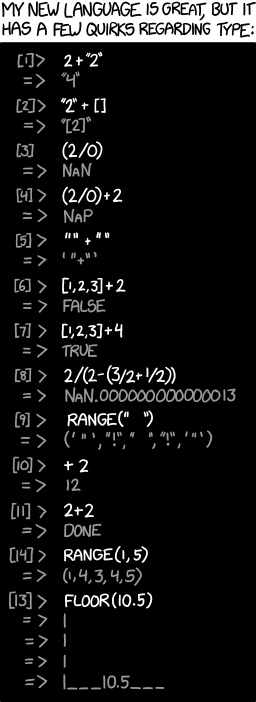
\includegraphics[width=.4\linewidth]{./gfx/xkcd-types}
	\caption[Eingabeschemata in anderen Programmiersprachen]{Eingabeschemata in anderen Programmiersprachen\newline Quelle: \url{https://xkcd.com/1537/}}
	\enquote{\texttt{colors.rgb('{}'blue'{}')} yields \texttt{'{}'\#0000FF'{}'}.
	 \texttt{colors.rgb('{}'yellowish blue'{}')} yields \texttt{NaN}. 
	 \texttt{colors.sort()} yields \texttt{'{}'rainbow'{}'}}
\end{figure}
%	\chapter{Schleifen}
\label{chp:loops}
\epigraph{
	Insanity: doing the same thing over and over again and expecting different results
}{Albert Einstein}

Computer können dazu benutzt werden, die immer gleichen (lästigen) Aufgaben wiederholt und in schneller Folge auszuführen. Es ist möglich, bei jeder Wiederholung einen einzelnen Eingabewert zu ändern und so \eg Berechnungen für einen ganzen Wertebereich durchzuführen, oder Messwerte von einem Gerät zu überwachen.

Zeichnet man ein \emph{Flussdiagramm} eines solchen Programms (wie in Abbildung \ref{fig:FlowBasicLoop}), so findet sich in der Regel ein Programmteil, der zur Vorbereitung dient und in gewohnter Weise \enquote{von oben nach unten} abgearbeitet wird. An diesen schließt sich ein Abschnitt an, der einige Male wiederholt werden soll, und daher im Flussdiagramm als Bogen dargestellt wird. Nach diesem Teil könnte die Ausgabe der Ergebnisse stattfinden, die wiederum in gewohnter \emph{linearer} Weise (also von oben nach unten) bearbeitet wird. 

Die Form dieses Flussdiagramms motiviert den Namen \emph{Schleife} für eine solche Struktur.

\begin{figure}[h!]
\begin{center}
\begin{tikzpicture}
    \node at (0, 3  ) (Input)      {Vorbereitung};
    \node at (0, 1.5) (Operations) {Wiederholungen};
    \node at (0, 0  ) (Output)     {Nachbereitung};
    
    \draw [->] (Input) -- (Operations);
    \draw [->] (Operations.south)arc(-160:160:1.0);		%start angle: stop angle : radius
    \draw [->] (Operations) -- (Output);
\end{tikzpicture}
\caption{Programmflussdiagramm mit Schleife} \label{fig:FlowBasicLoop}
\end{center}
\end{figure}

In der Regel ist die Zahl der Schleifendurchläufe an eine Bedingung geknüpft; genauso sind aber auch \emph{Endlosschleifen} möglich. In diesem Kapitel werden wir verschiedene Schleifentypen und ihre Anwendungsfelder kennen lernen.

\begin{hintbox}[Laufende Programme zum Beenden zwingen: \texttt{STRG + C}]
Macht man einen Fehler bei der Formulierung der Bedingung, so kann man unbeabsichtigt eine Endlosschleife erstellen. Ein solches Programm wird von sich selbst aus nie beendet. Wir können zu jeder Zeit aber das Beenden erzwingen, indem wir in der Konsole die Tastenkombination \texttt{STRG + C} drücken.
\end{hintbox}

\section{\inPy{while}-Loops}
\subsection{Grundstruktur}
Mit dem Schlüsselwort \inPy{while} wird ein Codeblock eingeleitet, der so lange wiederholt wird, bis eine Bedingung nicht mehr erfüllt ist, \ie bis ihr Wahrheitswert zu \inPy{False} ausgewertet wird. Die Syntax lautet:

\begin{codebox}[Syntax: \texttt{while} (1)]
\begin{minted}{python}
while Wahrheitswert :
    Schleifenkoerper
\end{minted}
\end{codebox}

Betrachten Sie hierzu folgendes Beispiel zum Zinseszins: \enquote{berechnet} wird, nach wie vielen Jahren ein Startkapital bei gegebenem Zinssatz über einen Grenzwert hinauswächst\footnote{Natürlich ließe sich dies auch über die Logarithmus-Funktion realisieren; hier aber soll die Funktionsweise von Schleifen gezeigt werden}.

\begin{codebox}[Beispiel: Zinseszins (1)]
\begin{minted}[linenos]{python}
capital  = float(input("Bitte geben Sie Ihr Startkapital ein: "))
interest = float(input("Bitte geben Sie den Zinssatz ein: "    ))
limit    = float(input("Bitte geben Sie Ihr Zielkapital ein :" ))

years    = 0

while capital < limit :
    capital *= 1 + interest
    years   += 1

print("Nach", years, "Jahren ist das Sparziel erreicht.")
\end{minted}
\end{codebox}

Nachdem die Variablen \inPy{capital, interest, limit} und \inPy{years} ihre Werte zugewiesen bekommen haben, wird überprüft, ob \inPy{capital < limit}. Wenn dies erfüllt ist, werden die Zeilen 8 und 9 ausgeführt. Danach springt die Codeausführung zurück zu Zeile 7. Es wird solange der Schleifenkörper in Zeile 8 und 9 wiederholt, bis die Bedingung in Zeile 7 nicht mehr erfüllt ist. Erst dann wird mit der Ausführung in Zeile 11 fortgesetzt. So erklärt sich folgendes Ausführungsbeispiel:

\begin{cmdbox}[Ausführungsbeispiel: Zinseszins (1)]
\begin{minted}{text}
Bitte geben Sie Ihr Startkapital ein: 100
Bitte geben Sie den Zinssatz ein: .1
Bitte geben Sie Ihr Zielkapital ein :300
Nach 12 Jahren ist das Sparziel erreicht.
\end{minted}
\end{cmdbox}

Der Schleifenkörper wird nie ausgeführt, wenn die Bedingung nicht bereits vor Beginn der Schleife erfüllt war. Geben Sie im obigen Beispiel etwa ein Startkapital ein, das größer als das Zielkaptital ist, so folgt die Ausgabe \texttt{Nach 0 Jahren ist das Sparziel erreicht.} Die Zeile \inPy{years += 1} wird nie ausgeführt.

\begin{hintbox}[Endlosschleifen]
Manchmal möchte man, dass ein Programm auf unbestimmte Zeit läuft. Code, der die Messwerte einer Wetterstation verarbeitet, soll dies vielleicth \enquote{für immer} tun. In diesem Fall bietet sich eine Endlosschleife an:
\begin{codebox}[Code: Endlosschleife]
\begin{minted}[linenos]{python}
while True:
  Anweisungen
\end{minted}
\end{codebox}
Da \inPy{True} eine Konstante ist, wird sich nichts daran ändern, dass sie immer eben zu \inPy{True} ausgewertet wird. Das Programm läuft bis in alle Ewigkeiten (oder zumindest, bis es vom Betriebssystem beendet wird). Üblicherweise enthält \inPy{Anweisungen} dann Code, der das Programm dennoch zu einem Ende führt. Diese Anweisungen könnten aber an komplexe Bedingungen geknüpft sein, die für die Form von \inPy{while} zu sperrig sind.
\end{hintbox}


\subsection{Eingriff in den Kontrollfluss}
Es gibt Situtaionen, wo die Ausführung einer Schleife an mehrere, voneinander unabhängige Bedingungen geknüpft sind. Dies lässt sich mit logischen Operatoren (Siehe Abschnitt \ref{sec:Booleans}) umsetzen. Häufig ist es aber übersichtlicher, das Schlüsselwort \inPy{break} in einem eigenen \inPy{if}-Block zu benutzen. Mit \inPy{break} wird der Schleifenkörper verlassen, die Ausführung wird hinter der Schleife fortgesetzt, ganz als ob die Bedingung hinter \inPy{while} selbst nicht mehr erfüllt wäre. Zusätzlich zur Übersichtlichkeit bietet diese \inPy{break}-Methode die Möglichkeit, an einem beliebigen Punkt innerhalb der Schleife zu prüfen, ob der Schleifenkörper verlassen werden soll.

\begin{codebox}[Beispiel: \texttt{break}]
\begin{minted}[linenos]{python}
count = 0
value = 0

while count < 12 :
    newValue = float(input("Bitte geben Sie einen weiteren Wert ein: "))
    value += newValue
    count += 1
  
    if value > 9000 :
        value = "over nine thousand!!"
        break
  
    print(
        "Bisheriger Gesamtwert nach Eingabe von", count, 
        "Werten:", value
    )

print("Gesamtwert:", value)
\end{minted}
\end{codebox}

Das Einlesen von \inPy{newValue} sowie die Updates an \inPy{value} und \inPy{count} werden bei jedem Durchlauf der Schleife durchgeführt. Die Ausgabe des Zwischenstandes (Zeilen 13-16) hingegen nur, wenn die Zweite Bedingung (\inPy{value > 9000}) nicht erfüllt war. So erklärt sich folgendes Ausführungsbeispiel:

\begin{cmdbox}[Ausführungsbeispiel: \texttt{break}]
\begin{minted}{text}
Bitte geben Sie einen weiteren Wert ein: 1
Bisheriger Gesamtwert nach Eingabe von 1 Werten: 1.0
Bitte geben Sie einen weiteren Wert ein: 50
Bisheriger Gesamtwert nach Eingabe von 2 Werten: 51.0
Bitte geben Sie einen weiteren Wert ein: 9000
Gesamtwert: over nine thousand!!
\end{minted}
\end{cmdbox}

Ähnlich kann \inPy{continue} benutzt werden, um einen Teil des Schleifenkörpers zu überspringen, ohne die Schleife selbst zu verlassen. Der Befehl \inPy{continue} springt also zur Überprüfung der \inPy{while}-Bedingung zurück:

\begin{codebox}[Beispiel: \texttt{continue}]
\begin{minted}[linenos]{python}
container = []

while len(container) < 3 :
    value = int(input("Bitte geben Sie eine gerade Zahl ein: "))
  
    if value % 2 :
        print(value, "ist ungerade und daher nicht zulässig.")
        continue
  
    container.append(value)
    print("Bisher eingegeben: ", container)
\end{minted}
\end{codebox}

\begin{cmdbox}[Ausführungsbeispiel: \texttt{continue}]
\begin{minted}{text}
Bitte geben Sie eine gerade Zahl ein: 2
Bisher eingegeben:  [2]
Bitte geben Sie eine gerade Zahl ein: 3
3 ist ungerade und daher nicht zulässig.
Bitte geben Sie eine gerade Zahl ein: 4
Bisher eingegeben:  [2, 4]
Bitte geben Sie eine gerade Zahl ein: 6
Bisher eingegeben:  [2, 4, 6]
\end{minted}
\end{cmdbox}

\begin{hintbox}[Garantierte erste Ausführung]
Wir können Endlosschleifen zusammen mit \inPy{break} nutzen, um zu garantieren, dass der Schleifenkörper mindestens einmal ausgeführt wird, unabhängig davon, ob die Schleifenbedingung zu Anfang bereits erfüllt war:
\begin{codebox}[Beispiel: \texttt{continue}]
\begin{minted}[linenos]{python}
while True:
    Schleifenkoerper
    if Bedingung :
        break
\end{minted}
\end{codebox}
Die Überprüfung auf \inPy{Bedingung} wird so an das Schleifenende geschoben.
\end{hintbox}


\subsection{\texttt{else} bei \texttt{while}}
Wie schon angesprochen wird der Schleifenkörper nicht ausgeführt, wenn die Bedingung schon vor der ersten Durchführung nicht erfüllt war. In diesem Fall kann ein optionaler \inPy{else}-Block ausgeführt werden:

\begin{codebox}[Syntax: \texttt{while} (2)]
\begin{minted}{python}
while Wahrheitswert :
    Schleifenkoerper
else :
    AlternativCode
\end{minted}
\end{codebox}

Betrachten wir dies an einem erweiterten Beispiel:
\begin{codebox}[Beispiel: Zinseszins (2)]
\begin{minted}[linenos]{python}
capital  = float(input("Bitte geben Sie Ihr Startkapital ein: "))
interest = float(input("Bitte geben Sie den Zinssatz ein: "    ))
limit    = float(input("Bitte geben Sie Ihr Zielkapital ein :" ))

years    = 0

while capital < limit :
    capital *= 1 + interest
    years   += 1
else :
    print("Das Startkapital ist bereits groß genug.")
  
print("Nach", years, "Jahren ist das Sparziel erreicht.")
\end{minted}
\end{codebox}

Die Zeile \texttt{Das Startkapital ist bereits groß genug.} wird genau dann ausgegeben, wenn für \inPy{capital} ein Wert größer oder gleich \inPy{limit} eingegeben wurde. Weiterhin wird für diesen Fall \texttt{Nach 0 Jahren ist das Sparziel erreicht.} als zweite Zeile ausgegeben.

\begin{warnbox}[Garantierte erste Ausführung mit \texttt{else}]
Statt der oben gezeigten Form mit \inPy{break} könnte auch mit \inPy{else} dafür gesorgt werden, dass der Schleifenkörper mindestens einmal ausgeführt wird. Hierzu kopiert man einfach den kompletten Code des Schleifenkörpers in den \inPy{else}-Block.

Dies erfüllt zwar seinen Zweck, ist aber eine Fehlerquelle und sollte vermieden werden. Wenn Sie später Codestellen ändern, müssen Sie auch daran denken, dieselben Änderungen im \inPy{else}-Block umzusetzen. Dies wird leicht vergessen.
\end{warnbox}

    
\section{\inPy{for}-Loops}
\subsection{Grundstruktur}
Schleifen mit \inPy{for} führen Code für jedes Element aus einer Datenstruktur wie in Kapitel \ref{chp:Containers} beschrieben aus. Nacheinander wird jedes Element des Containers über eine Hilfsvariable ansprechbar gemacht und dann Code ausgeführt, der von dieser Hilfsvariablen abhängig sein kann.

\begin{codebox}[Syntax: \texttt{for}]
\begin{minted}{python}
for Variable in Container :
    Schleifenkoerper
\end{minted}
\end{codebox}

Der Code lässt sich also fast wie englische Sprache lesen: \enquote{für jedes Objekt in \emph{Container} mache \emph{Schleifenkörper}}.

\begin{codebox}[Beispiel: \texttt{for} (1)]
\begin{minted}[linenos]{python}
tasklist = ["write the script", "drink some coffee", "drink some more coffee"]

print("Your tasks today:")
for task in tasklist :
    print("*", task)
\end{minted}
\end{codebox}

\begin{cmdbox}[Ausgabe: \texttt{for} (1)]
\begin{minted}{text}
Your tasks today:
* write the script
* drink some coffee
* drink some more coffee"
\end{minted}
\end{cmdbox}

Als \emph{Container} dienen besonders häufig \inPy{range}-Objekte. Wann immer eine durchzählbare Menge von Zahlen gebraucht wird, kann ein solches \inPy{range}-Objekt genutzt werden\footnote{Das folgende Beispiel und einige weitere enthalten die Option \inPy{sep=""}. Damit wird der Funktion \inPy{print} mitgeteilt, dass kein Leerzeichen zwischen den einzelnen Werten gedruckt werden soll. Vorerst können Sie diese Option ignorieren. In Kapitel \ref{chp:Funcs} wird diese Technik erklärt.}:

\begin{codebox}[Beispiel: \texttt{for} (2)]
\begin{minted}[linenos]{python}
print("the first 10 square numbers are:")
for i in range(10) :
    print(i, "² = ", i**2, sep="")
\end{minted}
\end{codebox}

\begin{cmdbox}[Ausgabe: \texttt{for} (2)]
\begin{minted}{text}
the first 10 square numbers are:
0² = 0
1² = 1
2² = 4
3² = 9
4² = 16
5² = 25
6² = 36
7² = 49
8² = 64
9² = 81
\end{minted}
\end{cmdbox}

\begin{hintbox}[Falls Sie von einer anderen Sprache kommen: Keine Indices]
Das Konzept einer for-Schleife existiert in fast allen Programmiersprachen. Häufig ist dort die Funktionalität jedoch auf Zahlen eingeschränkt. Will man \emph{über die Elemente eines Containers iterieren}, muss man dort die Schleife über die Indices laufen lassen. Das sieht dann beispielsweise so aus:

\begin{codebox}[Beispiel: \texttt{for} mit Indices]
\begin{minted}[linenos]{python}
tasklist = ["write the script", "drink some coffee", "drink more coffee"]
N = len(tasklist)

print("Your tasks today:")
for i in range(N) :
    print("*", tasklist[i])
\end{minted}
\end{codebox}

Dieses Beispiel funktioniert zwar, hat aber mehr Fehlerquellen. Man muss mindestens dafür sorgen, dass der Wert \inPy{N} zu jeder Zeit die korrekte Anzahl von Elementen in \inPy{tasklist} enthält. Sprachen wie C oder BASIC machen solche Strukturen leider nötig. In Python dagegen können wir diese Aufgabe getrost dem Interpreter überlassen.

Falls sie bereits eine andere Sprache kennen, sind sie es vielleicht gewohnt, for-Schleifen über Indices laufen zu lassen. Gewohnen Sie sich dies in Python ab. Nicht nur vermeiden Sie so eine Fehlerquelle; Ihr Code wird tatsächlich auch performanter, wenn Sie die \enquote{Python-Hausmittel} voll ausschöpfen.
\end{hintbox}

In einem \inPy{for}-Befehl können auch Container entpackt werden:
\begin{codebox}[Beispiel: \texttt{for} (3)]
\begin{minted}[linenos]{python}
books = [
    ("Frank Herbert", "Dune"), 
    ("Douglas Adams", "The Hitchhikers Guide To The Galaxy"),
    ("Randall Munroe", "What If"),
    ("Isaac Asimov", "Foundation"),
    ("Willy Russell", "Educating Rita"),
    ("Moving Pictures", "Terry Pratchett")
]

print("You should definitively read:")
for author, title in books :
    print("*", title, "by", author)
\end{minted}
\end{codebox}

\begin{cmdbox}[Ausgabe: \texttt{for} (3)]
\begin{minted}{text}
You should definitively read:
* Dune by Frank Herbert
* The Hitchhikers Guide To The Galaxy by Douglas Adams
* What If by Randall Munroe
* Foundation by Isaac Asimov
* Educating Rita by Willy Russell
* Moving Pictures by Terry Pratchett
\end{minted}
\end{cmdbox}

Natürlich \emph{müssen} Tupel \emph{nicht} enptackt werden:
\begin{codebox}[Beispiel: \texttt{for} (4)]
\begin{minted}[linenos]{python}
import math
vectors = [(1, 1), (4, 7), (-1, 2)]

for v in vectors :
  print("vector", v, "has length", math.hypot(v[0], v[1]))
\end{minted}
\end{codebox}

\begin{cmdbox}[Ausgabe: \texttt{for} (4)]
\begin{minted}{text}
vector (1, 1) has length 1.4142135623730951
vector (4, 7) has length 8.06225774829855
vector (-1, 2) has length 2.23606797749979
\end{minted}
\end{cmdbox}


\begin{hintbox}[Objekt und Index: \texttt{enumerate}]
Manchmal wird sowohl das Objekt als auch seine Position in der Liste benötigt. Mit der Funktion \inPy{enumerate} lässt sich ein Tupel aus genau diesen beiden Objekten erzeugen:

\begin{codebox}[Beispiel: \texttt{for} mit \texttt{enumerate}]
\begin{minted}[linenos]{python}
tasklist = ["write the script", "drink some coffee", "drink more coffee"]

print("Your tasks today:")
for i, task in enumerate(tasklist) :
    print(i + 1, ". ", task, sep="")
\end{minted}
\end{codebox}

\begin{cmdbox}[Ausgabe: \texttt{for} mit \texttt{enumerate}]
\begin{minted}{text}
Your tasks today:
1. write the script
2. drink some coffee
3. drink more coffee
\end{minted}
\end{cmdbox}

Beachten Sie, dass die Zahlen, wie von \inPy{enumerate} erzeugt bei \inPy{0} beginnen.
\end{hintbox}

\begin{hintbox}[Iteration über zwei Listen zugleich: \texttt{zip}]
Nicht selten müssen die Daten in zwei Listen zueinander in Bezug gesetzt werden. Stellen Sie sich beispielsweise vor, Sie haben zwei Messreihen aufgenommen, und wollen nun die Abweichungen dieser Messreihen berechnen. Hierzu können Sie den Ihnen bereits bekannten Befehl \inPy{zip} benutzen:

\begin{codebox}[Beispiel: \texttt{for} mit \texttt{zip}]
\begin{minted}[linenos]{python}
data1 = [1.7, 2.2, -4.1]
data2 = [1.8, 2.0, -3.8]

print("Difference in datasets:")
for i, t in enumerate(zip(data1, data2)) :
    print(
        "Datapoint ", i, ": ", t, 
        " differs by : ", t[0] - t[1], 
        sep=""
    )
\end{minted}
\end{codebox}

\begin{cmdbox}[Ausgabe: \texttt{for} mit \texttt{zip}]
\begin{minted}{text}
Datapoint 0: (1.7, 1.8) differs by : -0.10000000000000009
Datapoint 1: (2.2, 2.0) differs by : 0.20000000000000018
Datapoint 2: (-4.1, -3.8) differs by : -0.2999999999999998
\end{minted}
\end{cmdbox}
\end{hintbox}

Wie erwähnt können \emph{alle} Container für \inPy{for}-Schleifen verwendet werden, die wir aus Kapitel \ref{chp:Containers} kennen\footnote{In Kapitel \ref{chp:Classes} werden wir noch Möglichkeiten kennen lernen, weitere \emph{iterierbare} Objekte zu erstellen.}. Als Beispiel sei die Ausgabe eines \inPy{dict}s gezeigt:
\begin{codebox}[Beispiel: \texttt{for} mit \texttt{dict}s]
\begin{minted}[linenos]{python}
houseStark = {"Sigil" : "A grey direwolf on a white field",
              "Words" : "Winter Is Coming",
              "Seat"  : "Winterfell"}

print("Summary of House Stark:")
for key, value in houseStark.items() :
    print(key, ":\t", value, sep="")
\end{minted}
\end{codebox}

\begin{cmdbox}[Ausgabe: \texttt{for} mit \texttt{dict}s]
\begin{minted}{text}
Summary of House Stark:
Sigil:  A grey direwolf on a white field
Words:  Winter Is Coming
Seat:   Winterfell
\end{minted}
\end{cmdbox}


%\begin{hintbox}[Underscore]
%normally last result; in code usually obligatory forget.
%\end{hintbox}

\subsection{Eingriffe in den Kontrollfluss, \texttt{else}}
Auch bei \inPy{for} können die Befehle \inPy{break} und \inPy{continue} eingesetzt werden, und verhalten sich dort genauso, wie bei \inPy{while}. Außerdem existiert auch bei \inPy{for} eine optionale \inPy{else}-Klausel. Der Code hierin wird ausgeführt, wenn die \inPy{for}-Schleife normal zum Ende kam, also \emph{nicht} durch \inPy{break} abgebrochen wurde.

\begin{codebox}[Beispiel: \texttt{for} mit \texttt{break}{,} \texttt{continue} und \texttt{else}]
\begin{minted}[linenos]{python}
tasks = [
    ("hidden", "watch Fullmetal Alchemist"),
    ("open", "work very hard on Python"),
    ("open", "drink all the coffee")
]
search = ["watch", "work"]

for keyword in search :
    for ID, (state, task) in enumerate(tasks) :
        if state == "hidden" : continue
        if keyword in task :
            print(keyword, "was found in task ID", ID)
            break
    else :
        print(keyword, "was not found in the tasks.")
\end{minted}
\end{codebox}

\begin{cmdbox}[Ausgabe: \texttt{for} mit \texttt{break}{,} \texttt{continue} und \texttt{else}]
\begin{minted}{text}
watch was not found in the tasks.
work was found in task ID 1
\end{minted}
\end{cmdbox}

Machen Sie sich klar, was hier passiert: In der äußeren Schleife sorgen wir dafür, dass wir nacheinander nach zwei Begriffen in der Aufgabenliste suchen. Diese Begriffe werden mit \inPy{keyword} \enquote{greifbar gemacht}.

Für die innere Schleife betrachten wir ein Tupel aus einer ID und einem weiteren Tupel, das die Elemente von \inPy{tasks} umfasst. Hierfür verwenden wir die Symbole \inPy{ID}, \inPy{state} und \inPy{task}. Da \inPy{state} und \inPy{task} aus den Elementen von \inPy{tasks} gebildet werden (also für sich eine eigene Einheit bilden), müssen diese in Klammern gefasst werden.

Für jedes Element aus \inPy{tasks} wird zunächst der \inPy{state} betrachtet. Ist dieser gleich \inPy{"hidden"}, so wird das Element in der Analyse übersprungen (wir führen \inPy{continue} aus.) Andernfalls wird geprüft, ob \inPy{keyword} in der Aufgabenbeschreibung \inPy{task} gefunden wurde. Ist dies der Fall, so ist die Analyse des aktuellen Elements der Aufgabenliste \inPy{tasks} abgeschlossen (wir führen \inPy{break} aus), und das nächste \inPy{keyword} kann betrachtet werden.

In dem Fall, wo das \inPy{keyword} gefunden werden kann (also \eg für \inPy{"work"}) wird also ein \inPy{break} ausgelöst und folglich der Code bei \inPy{else} übersprungen. Dagegen löst das \inPy{keyword "watch"} den \inPy{if}-Block in Zeile 11 nicht aus (da die Prüfung mit Zeile 10 bereits übersprungen wird). Daher läuft die \inPy{for}-Schleife vollständig durch, und der \inPy{else}-Block wird ausgeführt.

\section{List Comprehension}
Stellen Sie sich vor, Sie brauchen eine Liste mit den Quadraten aller geraden Ganzzahlen. Sie können diese Aufgabe jetzt schon so lösen:

\begin{codebox}[Beispiel: \texttt{for} zum Erstellen einer Liste]
\begin{minted}[linenos]{python}
evenSquares = []
N = 20

for i in range(2, N, 2) :
    evenSquares.append(i**2)

print(evenSquares)
\end{minted}
\end{codebox}

\begin{cmdbox}[Ausgabe: \texttt{for} zum Erstellen einer Liste]
[4, 16, 36, 64, 100, 144, 196, 256, 324]
\end{cmdbox}

Dieselbe Konstruktion können Sie verkürzt auch schreiben als:
\begin{codebox}[Beispiel: List Comprehension]
\begin{minted}[linenos]{python}
N = 20
evenSquares = [ i**2 for i in range(2, N, 2) ]
print(evenSquares)
\end{minted}
\end{codebox}

Die Abstrakte Syntax lautet also:
\begin{codebox}[Syntax : List Comprehension (1)]
\begin{minted}[linenos]{python}
variable = [ expression for element in iterable ]
print(evenSquares)
\end{minted}
\end{codebox}
Dabei sind
\begin{itemize}
\item \inPy{iterable} ein beliebiger Datencontainer, wie in allen vorigen Beispielen
\item \inPy{element} eine Variable, über die nacheinander die einzelnen Elemente aus \inPy{iterable} durchgelesen werden. Auch hier können Tupel entpackt werden. In
	diesem Fall müssen entsprechend mehrere Variablen genannt werden.
\item \inPy{expression} ist ein beliebiger Ausdruck, der die zu erzeugenden Listenelemente beschreibt.
\end{itemize}

List Comprehension kann auch ineinander verschachtelt werden (wird dann aber schnell unübersichtlich). Die folgende Zeile erzeugt die sogenannte \enquote{Telefonmatrix}:

\begin{codebox}[Beispiel: Telefonmatrix]
\begin{minted}[linenos]{python}
telephone = [
    [3 * row + column + 1 for column in range(3)]
    for row in range(3)
]

for line in telephone :
    print(line)

print(telephone)
\end{minted}
\end{codebox}

Der Code erzeugt also eine \emph{Liste von Listen}:
\begin{cmdbox}[Ausgabe: Telefonmatrix]
\begin{minted}{text}
[1, 2, 3]
[4, 5, 6]
[7, 8, 9]
[[1, 2, 3], [4, 5, 6], [7, 8, 9]]
\end{minted}
\end{cmdbox}

\begin{hintbox}[Sprechende Variablennamen]
Im obigen Beispiel \emph{Telefonmatrix} taucht die Variable \inPy{row} zum ersten Mail in Zeile 2 auf, obwohl erst in Zeile 3 erklärt wird, welche Werte \inPy{row} haben wird, oder um welche Art von Werten (Integer, Fließkommazahlen, Strings, Container, ...) es sich überhaupt handelt. \emph{Strukturell} kommen wir also in die Gefahr von schwer lesbarem Code, und haben damit eine Fehlerquelle. Durch die Benennung der Variablen ist aber dennoch schnell klar, was hier passiert. Die Variablen \inPy{row} und \inPy{column} bezeichnen die Nummer von Zeile und Spalte einer Matrix, sind also Integers zwischen 0 und einer Obergrenze, die sich aus der Größe der Matrix ergibt.

Solche Überlegungen zur Benennung der Objekte sind extrem wichtig in auch nur mittelgroßen Projekten. Geben Sie nicht der Versuchung nach, Variablen aus Bequemlichkeit einfach \inPy{a, b, c, ...} zu nennen, sondern überlegen Sie, welche Art von Information darin abgelegt werden soll, und schreiben dies dann auch aus! Auch Abkürzungen sollten vermieden werden, da sich hierbei oft Fehler einschleichen. Hieß die Variable nun \inPy{numElmL} oder \inPy{nel} oder \inPy{nElements}? Diese Frage stellt sich nicht, wenn Sie sich die kleine Mühe machen, konsequent \inPy{numberElementsList} zu tippen; Sie sparen sich dadurch die große Mühe, häufig zurück zu scrollen und Fehler auszumerzen, die sich daraus ergeben, dass Sie mal \inPy{numElmL} und mal \inPy{numElml} getippt haben.
\end{hintbox}

Bei der List Comprehension können Sie auch die Aufnahme eines Wertes in die Ergebnis-Liste an eine Bedingung knüpfen. Sie erreichen dies, indem Sie einfach eine \inPy{if}-Klausel anfügen:
\begin{codebox}[Syntax : List Comprehension (2)]
\begin{minted}[linenos]{python}
variable = [ expression for element in iterable if condition ]
print(evenSquares)
\end{minted}
\end{codebox}

Als Beispiel soll eine Liste aller Primzahlen bis zu einer Obergrenze \inPy{N} berechnet werden. Wir nutzen dazu aus, dass eine Primzahl exakt zwei Ganzzahl-Teiler hat. Wir erstellen also zuerst für jede Zahl zwischen 2 und \inPy{N} alle Ganzzahl-Teiler, und akzeptieren nur solche Zahlen in unserem Ergebnis, bei dem diese Liste der Teiler die Länge \inPy{2} hat\footnote{Der gezeigte Code ist sowohl bezüglich Rechenzeit als auch bezüglich Speicherbedarf schlecht, illustriert aber schön die Technik, um die es uns hier geht.}.

\begin{codebox}[Beispiel: List Comprehension mit Bedingung]
\begin{minted}[linenos]{python}
N = 100
primeNumbers = [
  i for i in range (2, N)       # übernehme alle Zahlen i zwischen 2 und N ...
  if len (                      # ... für die die die Anzahl der Teiler ...
    [j for j in range (1, i+1)  # ... (d.h. die Zahlen zwischen 1 und i ...
    if i % j == 0]              # ... die i ganzzahlig teilen) ...
  ) == 2                        # ... gleich 2 ist.
]

print(primeNumbers)
\end{minted}
\end{codebox}

\begin{cmdbox}[Ausgabe: List Comprehension mit Bedingung]
[2, 3, 5, 7, 11, 13, 17, 19, 23, 29, 31, 37, 41, 43, 47, 53, 59, 61, 67, 71, 73, 79, 83, 89, 97]
\end{cmdbox}


List Comprehension lässt sich auch für \inPy{set}s und \inPy{dict}s umsetzen. Die Synax verlangt dann nur eine minimale Anpassung:
\begin{codebox}[Syntax : List Comprehension (3)]
\begin{minted}[linenos]{python}
setVariable  = {       expression for element in iterable if condition }
dictVariable = { key : expression for element in iterable if condition }
\end{minted}
\end{codebox}
Natürlich sind die \inPy{if}-Klauseln auch für \inPy{set}s und \inPy{dict}s optional.

\begin{codebox}[Beispiel: List Comprehension für \texttt{set}s und \texttt{dict}s]
\begin{minted}[linenos]{python}
# Die ersten 10 Quadratzahlen als set:
print( {i**2 for i in range (10)} )
# Die ersten 10 Quadratzahlen als dict
print( {i : i**2 for i in range (10)} )
\end{minted}
\end{codebox}

\begin{cmdbox}[Ausgabe: List Comprehension für \texttt{set}s und \texttt{dict}s]
\begin{minted}{text}
{0, 1, 64, 4, 36, 9, 16, 49, 81, 25}
{0: 0, 1: 1, 2: 4, 3: 9, 4: 16, 5: 25, 6: 36, 7: 49, 8: 64, 9: 81}
\end{minted}
\end{cmdbox}

\begin{hintbox}[Aufwändige Berechnungen vorbereiten]
In wissenschaftlichen Simulationen treten manche Ausdrücke wie $e^k$ gehäuft für die immer gleichen Werte von $k$ auf. Anstatt die Exponentialfunktion immer wieder neu auszuwerten lohnt es sich oft, die Werte einmal in einer Liste vorzubereiten und so den Rechenaufwand zu minimieren. List Comprehension bietet sich hierzu perfekt an.

Für besonders gleichmäßige Verteilungen (\ie wenn $k$ alle Ganzzahlen zwischen $0$ und einer Obergrenze sind) sollten \inPy{list}s verwendet werden, da diese leichter ausgelesen werden können. Allgemeinere Lookup-Tables lassen sich gut in \inPy{dict}s abbilden.
\end{hintbox}
%	\chapter{Funktionen}
\label{chp:Funcs}
\epigraph{
	Before software can be reusable it first has to be usable.
}{Ralph Johnson}

Viele Aufgaben wiederholen sich oder lassen sich verallgemeinern. Folgender Code berechnet beispielsweise den Wert von Eulers Zahl, also $\exp(1)$, kann aber auch dazu verwendet werden, andere Potenzen von $e$ zu finden:

\begin{codebox}[Beispiel: Exponentialfunktion]
\begin{minted}[linenos]{python}
x0           = 1.0
x            = 1.0
denominator  = 1.0
EulersNumber = 1.0
iterations   = 10

for k in range(1, iterations) :
  x            *= x0
  denominator  *= k
  EulersNumber += x / denominator

print ("exp(", x0, ") is approximately ", EulersNumber, sep = "")
\end{minted}
\end{codebox}

Nun ist es zwar schön, eine solche allgemeine Rechenvorschrift zu haben; wir müssen nur den Wert für \inPy{x0} in der ersten Zeile austauschen, und erhalten ein neues Ergebnis. Wollen wir aber an mehreren Stellen die Exponentialfunktion verwenden, so müssten wir diesen Code jedes Mal kopieren und neu einfügen. Schlimmer noch: sollte uns auffallen, dass wir im obigen Code einen Fehler gemacht haben, so müssen wir diesen \emph{für jede Kopie separat} ausmerzen. Und selbst, wenn wir auf Anhieb perfekt gearbeitet haben, \enquote{belegt} unser Code jetzt \ua die Symbole \inPy{x} und \inPy{x0}. Projekte, die diesen Code verwenden wollen, müssen also andere Namen finden.

Natürlich wissen Sie, dass es im Modul \inPy{math} die \emph{Funktion} \inPy{math.exp} gibt, die ebenfalls die Exponentialfunktion berechnet, aber ohne all diese lästigen Nebeneffekte auskommt. Hier sollen Sie lernen, wie dies möglich ist, und wie Sie solche Funktionen selbst erstellen.

\section{Grundlagen}
Funktionen sind \enquote{abgetrennte Codebereiche}, die unabhängig vom restlichen Code ausgeführt werden. In eine Funktion können Argumente (oft auch Parameter genannt) eingespeist werden (man spricht von \emph{übergeben}), und ein Ergebnis wird von  \emph{zurückgegeben}. Zur Berechnung dieses Ergebnisses wird normaler Code ausgeführt; dieser verhält sich aber \enquote{wie in einer Box}, \ie verwendet seine eigenen, \emph{lokalen} Variablen. Diese können dieselben Namen tragen wie Variablen an anderen Stellen Ihres Programms; nichts desto trotz sind die Variablen in einer Funktion unabhängig vom restlichen Code. (Ebenso, wie es zwei Menschen mit dem Namen \emph{Theophrastus} geben kann\footnote{citation needed}, die aber dennoch zwei getrennte Personen sind, können also auch zwei Variablen mit demselben Namen vorliegen, ohne \emph{dieselbe} Variable zu sein.)

Ein solcher Codebereich wird eingeleitet durch eine \inPy{def}-Zeile und wird durch Einrückung vom restlichen Code abgetrennt, ähnlich, wie wir das schon von \inPy{if}-Blöcken und \inPy{for}-Schleifen kennen:

\begin{codebox}[Syntax: Funktionen]
\begin{minted}{python}
def Funktionsname (Parameterliste) :
  normaler Code
  ...
  return Ergebnis
\end{minted}
\end{codebox}

Mit \inPy{Parameterliste} ist eine durch Kommata getrennte Liste von Variablennamen. Über diese Variablennamen werden \enquote{Informationen von außen in die Funktion eingeschleust} (Übergabe von Werten). Verstehen Sie die Parameterliste als einen Punkt, an dem Variablen angelegt werden. Die Werte dieser Variablen werden beim Aufruf der Funktion festgelegt, und können in der Funktion wie normale Variablen verwendet werden. Eine Parameterliste kann auch leer sein. In dem Fall müssen aber immer noch  leere Klammern () gesetzt werden.

Wie besprochen steht innerhalb einer Funktion Code, wie sie ihn schon kennen bzw. noch kennenlernen werden. Alle Mittel, die Sie bisher kennengelernt haben auch auch solche, wie wir sie im Weiteren noch besprechen, können auch innerhalb von Funktionen verwendet werden.

In der Regel soll eine Funktion ein Ergebnis berechnen, \eg den Wert der Exponentialfunktion. Dieses Ergebnis wird mit dem Befehl \inPy{return} zurück an das Hauptprogramm geschickt und zugleich die Funktion verlassen. Aller Code in der Funktion, der hinter \inPy{return} steht, wird also ignoriert. Eine Funktion darf durchaus mehrere \inPy{return}-Anweisungen haben. Sinnvoll kann das sein, wenn eine Fallunterscheidung gemacht wird (\eg mit \inPy{if}). Genauso ist es auch zulässig, überhaupt keine \inPy{return}-Anweisung zu benutzen. Stellen Sie sich zum Beispiel eine Funktion vor, die lediglich eine formatierte Ausgabe auf dem Bildschirm bewirken soll. Hier wird kein Ergebnis berechnet. Entsprechend kann auch die \inPy{return}-Anweisung entfallen.

\emph{Aufgerufen} (\ie ausgeführt) wird die Funktion durch Nennung ihres Namens. In Klammern dahinter werden die Werte aufgeführt, die über die Parameterliste an die Funktion übergeben werden sollen. Für jede Variable der Parameterliste muss auch ein Wert angegeben werden. Ist die Parameterliste leer, so müssen dennoch leere Klammern () beim Funktionsaufruf stehen.

Ein Funktionsaufruf macht also mehrere Dinge:
\begin{itemize}
\item Eine \emph{Kopie} der Werte in der Parameterliste wird an die Funktion übergeben
\item Die Programmausführung springt in die Funktion
\item Nach Ende der Funktion wird das Programm an der ürsprünglichen Stelle fortgeführt.
\end{itemize}
Nach Ende des Funktionsaufrufs wird an der aufrufenden Stelle ein Wert erhalten (eben der Rückgabewert der Funktion). Dieser kann in einer Variablen gespeichert werden, oder an andere Funktionen weitergegeben werden.

\begin{codebox}[Beispiel: Exponentialfunktion als Funktion]
\begin{minted}[linenos]{python}
def expFunction(x0) :
  x           = 1.0
  denominator = 1.0
  result      = 1.0
  iterations  = 10
  
  for k in range(1, iterations) :
    x            *= x0
    denominator  *= k
    result += x / denominator
    
  return result

EulersNumber = expFunction(1.0)          # Aufruf, Speichern in Variable
print("Eulers Number is", EulersNumber)
print("e³ =", expFunction(3.0))          # Weitergabe an andere Funktion
\end{minted}
\end{codebox}

\begin{cmdbox}[Ausgabe: Exponentialfunktion als Funktion]
\begin{minted}{text}
Eulers Number is 2.7182815255731922
e³ = 20.063392857142855
\end{minted}
\end{cmdbox}

Wird kein Rückgabewert genannt, so weist Python automatisch den Pseudo-Rückgabewert \inPy{None} zu. Es handelt sich dabei um eine Konstante, die eben genau für die Abwesenheit eines Wertes steht, und sollte auch nicht mit dem Text \inPy{"None"} verwechselt werden.
\begin{codebox}[Beispiel: Funktion \enquote{ohne} Rückgabewert]
\begin{minted}[linenos]{python}
import math

def printBoxed(text, boxSize) :
  # Draws text in a box like:
  #
  # +-----------+
  # |   text    |
  # +-----------+
  
  lenText     = len(text)
  countSpaces = boxSize - lenText - 2        # 2 spaces for |borders|
  spacesLeft  = math.floor(countSpaces / 2)  # round down
  spacesRight = math.ceil (countSpaces / 2)  # round up
  
  print("+" +               (boxSize - 2) * "-"           + "+")
  print("|" + spacesLeft * " " + text + spacesRight * " " + "|")
  print("+" +               (boxSize - 2) * "-"           + "+")
  
reVal = printBoxed("Don't forget to be awesome!", 60)
print("The function returned:" , reVal)
\end{minted}
\end{codebox}

\begin{cmdbox}[Ausgabe: Funktion \enquote{ohne} Rückgabewert]
\begin{minted}{text}
+----------------------------------------------------------+
|               Don't forget to be awesome!                |
+----------------------------------------------------------+
The function returned: None
\end{minted}
\end{cmdbox}

Wie erwähnt wird die Ausführung der Funktion sofort beendet, sobald der Interpreter auf eine \inPy{return}-Anweisung stößt. Daher haben die Zeilen 4 und 7 im folgenden Beispiel keinerlei Auswirkung:
\begin{codebox}[Beispiel: Funktion mit mehreren \texttt{return}-Anweisungen]
\begin{minted}[linenos]{python}
def max (a, b) :
  if a > b :
    return a
    print("this line will never be executed")
  else :
    return b
    print("and neither will this one")

print(max(1, 2))
print(max(2, 1))
\end{minted}
\end{codebox}

\begin{cmdbox}[Ausgabe: Funktion mit mehreren \texttt{return}-Anweisungen]
\begin{minted}{text}
2
2
\end{minted}
\end{cmdbox}

Wichtig ist, immer im Kopf zu behalten, dass die Variablen, die in einer Funktion benuzt werden, vom restlichen Programm unabhängig sind. Es darf also sich widersprechende Definitionen geben; die Definitionen gelten nur jeweils innerhalb einer Funktion:

\begin{codebox}[Beispiel: Gleiches Symbol{,} unterschiedliche Inhalte]
\begin{minted}[linenos]{python}
def func() :
  a = 7
  print("in func: a =", a)

a = 999
print("on module level: a =", a)
func()
print("on module level: a =", a)
\end{minted}
\end{codebox}

\begin{cmdbox}[Ausgabe: Gleiches Symbol{,} unterschiedliche Inhalte]
\begin{minted}{text}
on module level: a = 999
in func: a = 7
on module level: a = 999
\end{minted}
\end{cmdbox}

Das \inPy{a} in \inPy{func} erhält also seine eigene Speicherstelle. Je nach Kontext sucht der Python-Interpreter aus, ob die \inPy{func}-Speicherstelle oder die Modul-Level-Speicherstelle mit dem Symbol \inPy{a} gemeint ist.

\section{By-Value- und By-Reference-Übergabe}
Wir hatten festgestellt, dass die Variablen, die wir in einer Funktion verwenden, vom restlichen Coee abgetrennt sind. Wie aber verhält es sich mit den Parametern?

Sehen wir uns dazu folgenden Code an:
\begin{codebox}[Beispiel: Übergabe von Referenz by Value]
\begin{minted}[linenos]{python}
def Vercingetorix(data) :
  data.append(1)
  data = data + [2]
  print("in Vercingetorix: data =", data)

data = []
Vercingetorix(data)
print("on module level: data =", data)
\end{minted}
\end{codebox}
Oben wurde bereits gesagt, dass bei einem Funktionsaufruf eine \emph{Kopie} des Originalobjekts (hier also \inPy{l}) an die Funktion übergeben wird. Dann würden wir also erwarten, dass in Zeile 8 die Liste \inPy{l} wieder unverändert als leere Liste vorliegt. Kurioserweise lautet die Ausgabe aber:

\begin{cmdbox}[Ausgabe: Übergabe von Referenz by Value]
\begin{minted}{text}
in Vercingetorix: data = [1, 2]
on module level: data = [1]
\end{minted}
\end{cmdbox}

Wie lässt sich dies erklären?

In Abschnitt \ref{sec:MemoryModel} hatten wir uns klar gemacht, dass Variablen in Python in Wirklichkeit primär die \emph{Adressen} der eigentlichen Information speichert. Diese Adresse wird auch als Kopie übergeben. In Zeile 2 erteilen wir nun den Befehl, an die Liste an der Stelle \inPy{data} die Zahl 1 anzuhängen. Die Liste wird dadurch im Speicher nicht verschoben; daher sehen wir später in Zeile 8 das Ergebnis dieser Änderung.

In Zeile 3 dagegen wird eine \emph{neue} Liste berechnet (nämlich \inPy{[1, 2]}). Diese neue Liste wird an einer eigenen Speicherstelle angelegt, überschreibt also nicht die alten Daten an der Adresse \inPy{data}. Wir speichern in Zeile 3 die Adresse in der \emph{lokalen} Variablen \inPy{data}. Das bedeutet, die Funtion \inPy{Vercingetorix} weiß nun nicht mehr, wo die Original-Liste sich befindet, sondern kann nur noch die Liste \inPy{[1 ,2]} ausgeben -- und dies geschieht auch in Zeile 4. Die ursprüngliche Liste besteht aber weiterhin. Wo diese sich befindet, ist immer noch in der Variablen \inPy{data} des Modul-Levels gespeichert. Wir sehen daher in Zeile 8 das Ergebnis von \inPy{append} (da dies die Adresse von \inPy{data} nicht verändert hat), nicht aber das Ergebnis von \inPy{data = data + [2]} (da hierfür eine neue Liste angelegt wurde).

\begin{tcolorbox}[title=Speicherbild]
\begin{center}
\begin{tikzpicture}
  [ 
    cell/.style={text width=8mm,
      text height=4mm, draw=black, inner sep=1mm},
    ld/.style={draw=blue,shorten >=2pt,->}
  ]
  \node (a1) at (0,4) [cell] {\ttfamily ...};
  \node (a2) at (1,4) [cell] {\ttfamily  []};
  \node (a3) at (2,4) [cell] {\ttfamily ...};
  \node (a4) at (3,4) [cell] {\ttfamily ...};
  \node (a5) at (4,4) [cell] {\ttfamily ...};
  \node (a6) at (5,4) [cell] {\ttfamily ...};

  \node (b1) at (0,2) [cell] {\ttfamily ...};
  \node (b2) at (1,2) [cell] {\ttfamily [1]};
  \node (b3) at (2,2) [cell] {\ttfamily ...};
  \node (b4) at (3,2) [cell] {\ttfamily ...};
  \node (b5) at (4,2) [cell] {\ttfamily ...};
  \node (b6) at (5,2) [cell] {\ttfamily ...};

  \node (c1) at (0,0) [cell] {\ttfamily ...};
  \node (c2) at (1,0) [cell] {\ttfamily [1]};
  \node (c3) at (2,0) [cell] {\ttfamily ...};
  \node (c4) at (3,0) [cell] {\ttfamily ...};
  \node (c5) at (4,0) [cell] {\ttfamily ...};
  \node (c6) at (5,0) [cell] {\ttfamily [1,2]};

%  \node (labelMem) at (8,  1) {Symbole im Code};
%  \node (labelMem) at (8,  0) {Werte im Speicher};
%  \node (labelMem) at (8, -1) {Adressen};
  
  \node (A1) [below=2mm of a1]             {\tiny 0x27ff};
  \node (A2) [below=2mm of a2, color=teal] {\tiny 0x2800};
  \node (A3) [below=2mm of a3]             {\tiny 0x2801};
  \node (A4) [below=2mm of a4]             {\tiny 0x2802};
  \node (A5) [below=2mm of a5]             {\tiny 0x2803};
  \node (A6) [below=2mm of a6]             {\tiny 0x2804};
  
  \node (B1) [below=2mm of b1]             {\tiny 0x27ff};
  \node (B2) [below=2mm of b2, color=teal] {\tiny 0x2800};
  \node (B3) [below=2mm of b3]             {\tiny 0x2801};
  \node (B4) [below=2mm of b4]             {\tiny 0x2802};
  \node (B5) [below=2mm of b5]             {\tiny 0x2803};
  \node (B6) [below=2mm of b6]             {\tiny 0x2804};
  
  \node (C1) [below=2mm of c1]             {\tiny 0x27ff};
  \node (C2) [below=2mm of c2, color=teal] {\tiny 0x2800};
  \node (C3) [below=2mm of c3]             {\tiny 0x2801};
  \node (C4) [below=2mm of c4]             {\tiny 0x2802};
  \node (C5) [below=2mm of c5]             {\tiny 0x2803};
  \node (C6) [below=2mm of c6, color=blue] {\tiny 0x2804};

  \node (main1) [below=0mm of A2, color=teal] {\scriptsize Adresse von \texttt{data} in Modul-Level und in \texttt{Vercingetorx}};
  \node (main2) [below=0mm of B2, color=teal] {\scriptsize Adresse von \texttt{data} in Modul-Level und in \texttt{Vercingetorx}};
  \node (main3) [below=0mm of C2, color=teal] {\scriptsize Adr. von \texttt{data} in Modul-Level};
  \node (func)  [below=0mm of C6, color=blue] {\scriptsize Adr. von \texttt{data} in \texttt{Vercingetorix}};
  
  \draw [->] (a6.east)arc(120:-115:1.0);		%start angle: stop angle : radius  
  \node (step1) at (9,3) {\texttt{data.append(1)}};
  \draw [->] (b6.east)arc(120:-115:1.0);
  \node (step1) at (9,1) {\texttt{data = data + [2]}};
\end{tikzpicture}
\end{center}
\end{tcolorbox}


Durchdenken wir nun auch dieses Beispiel:
\begin{codebox}[Beispiel: Übergabe von Immutables]
\begin{minted}[linenos]{python}
def Vercingetorix(data) :
  data = 2
  print("in Vercingetorix: data =", data)

data = 1
Vercingetorix(data)
print("on module level: data =", data)
\end{minted}
\end{codebox}

\begin{cmdbox}[Ausgabe: Übergabe von Immutables]
\begin{minted}{text}
in Vercingetorix: data = 2
on module level: data = 1
\end{minted}
\end{cmdbox}

Wir erinnern uns, dass \inPy{1} ein Wert vom Typ \inPy{int} und damit \emph{immutable} ist. Der Wert an der Stelle \inPy{data} darf also nicht verändert werden. Wenn nun also Zeile 2 verlangt, den neuen Wert \inPy{2} \enquote{in \inPy{data}} zu speichern, so wird eine neue Speicherstelle angelegt, und deren Adresse in der Instanz von \inPy{data} in \inPy{Vercingetorix} gespeichert.

\begin{hintbox}[Speicherstruktur von \texttt{list}s]
Die oben gezeigten Speicherbilder sind eine Vereinfachung der Realität. Wie erwähnt kann jede Zelle des Speichers nur ein einziges Byte fassen, also nicht einmal einen ganzen \inPy{int}-Wert. Stattdessen finden Sie dort einen \emph{descriptor}, also ein Datenpaket, das unter anderem aus einer Ganzzahl (Anzahl der Elemente in der Liste) und einem Pointer (tatsächlicher Speicherort des ersten Elements der Liste, also eine Adresse) enthält. Dadurch bleibt die Adresse \inPy{data} konstant, selbst wenn der Listeninhalt \enquote{umziehen} muss.

In systemnahen Sprachen wie C müssen Sie das mit im Auge behalten. Bei der Arbein in Python dagegen können Sie sich weit mehr auf \enquote{das Große und Ganze} konzentrieren.
\end{hintbox}

\section{Scopes, \inPy{global}}
Bisher habe ich Ihnen verschwiegen, dass 

\begin{codebox}[Beispiel: lokale und globale Variablen]
\begin{minted}[linenos]{python}
foo = "foo"
bar = "bar"

def Vercingetorix() :
  foo = "fu"        # local variable
  
  global bar        # use the 'bar' from module level
  bar = "baz"

  print("Vercingetorix: foo =", foo)
  print("Vercingetorix: bar =", bar)

Vercingetorix()

print("on module level: foo =", foo)
print("on module level: bar =", bar)
\end{minted}
\end{codebox}
\begin{cmdbox}[Ausgabe: Übergabe von Immutables]
\begin{minted}{text}
Vercingetorix: foo = fu
Vercingetorix: bar = baz
on module level: foo = foo
on module level: bar = baz
\end{minted}
\end{cmdbox}


\section{Default Args}
\section{Variardic}
\section{Lambdas}

%	\chapter{Klassen}
\label{chp:Classes}
\epigraph{
	What's the object-oriented way to wealth? -- Inheritance
}{Anonymous}

In ihrem Grundaufbau sind Computer Maschinen, die mit \emph{einzelnen Zahlen} umgehen. \emph{Gruppen} von Zahlen sind alles, was wir brauchen, um unsere Welt zu beschreiben\footnote{Ich bin gerne zu einer philosophischen Diskussion über diese Aussage bereit. Für diesen Kurs wollen wir aber zumindest annähern, dass Zahlen zur Beschreibung von Dingen genügen, die wir mit einem Computer bearbeiten wollen}. Dazu müssen diese Zahlen aber eine gewisse Ordnung und Beziehung zueinander haben und wir brauchen eine geeignete Methode zur Interpretation dieser Zahlen. Die Zahlen 98, 108, 117, 101 können zum Beispiel \emph{in dieser Reiheinfolge} als ASCII-Codes der Buchstaben des Wortes \emph{blue} interpretiert werden; es könnten aber auch die Hausnummern der Adressen meiner ersten vier Lebensgefährtinnen sein\footnote{Sind sie nicht. Ich kann mich nur an die Hausnummer meiner vierten Freundin erinnern (es war die 12), und meine erste Freundin hat so weit von der nächsten Stadt gelebt, dass ich mir nicht sicher bin, ob das Haus überhaupt eine Hausnummer hatte.}.

Für Texte haben wir den Datentyp \inPy{string} kennengelernt. Hinter dem Datentypen steht eine aufwändige Maschinerie, die eben genau diese Ordnung und Interpretation von Zahlengruppen bietet. In diesem Kapitel wollen wir uns damit beschäftigen, eigene solche Konstrukte zu erschaffen: Wir erstellen hier \emph{Klassen}.

\section{Klassen als Container}
Zunächst sollten Sie sich eine Klasse als Datencontainer vorstellen, wie wir sie schon in Kapitel \ref{chp:Containers} kennengelernt haben\footnote{Tatsächlich sind die dort gezeigten Datentypen Beispiele für Klassen}. Dort wurden mehrere \eg Werte zu einem kompakten \inPy{dict} zusammengefasst. Um einen dieser zusammen gepackten Werte zu greifen, brauchten wir einen \emph{Schlüssel}.

Klassen haben in dieser Hinsicht eine ähnliche Struktur: Sie sind eine Sammlung von Attributen, zu denen man Werte speichern kann. Die Attribute einer Klasse richten sich natürlich danach, was modelliert werden soll. Beispielsweise könnten wir uns die Aufgabe stellen, meine Exfreundinnen mit Python zu analysieren. Attribute können dann so etwas sein wie \emph{Name}, \emph{Körpergröße}, \emph{positive Eigenschaften} oder \emph{negative Eigenschaften}.

Wir können uns in dem Kontext eine Tabelle vorstellen, in der ich meine Verflossenen auflisten könnte. Die Spaltenüberschriften dieser Tabelle wären dann die Attribute. Jede Zeile dieser Tabelle nennen wir eine \emph{Instanz} der Klasse. Eine Instanz beschreibt in diesem Fall also einen konkreten Menschen, der (unter anderem) durch die Attribute \emph{name}, \emph{height}, \emph{upsides} und \emph{downsides} beschrieben werden kann. Eine Instanz braucht außerdem noch ein \emph{Symbol}, über den klar wird, welche Zeile der Tabelle gemeint ist (schließlich ist es zumindest denkbar, dass zwei gleich große Menschen mit demselben Namen existieren, an denen ich dieselben Vorzüge und Nachteile sehe).

\begin{tcolorbox}[title=Eine Liste von Liebschaften]
\begin{center}
\begin{tabular}{c|ccp{.3\linewidth}p{.3\linewidth}}
	\textbf{Symbol} & \textbf{Name} & \textbf{Height} & \textbf{Upsides}                                 & \textbf{Downsides} \tabcrlf
	\texttt{gf1}    & Steffie       & 1.65 m          & intelligent, beautiful, has a dog                & too attached to her mother, 
																																																				doesn't like meeting people \tabcrlf
	\texttt{gf2}    & Arista        & 1.60 m          & very intelligent, beautiful, good taste in music & doesn't like coffee, doesn't like coding \tabcrlf
	\texttt{gf3}    & Katja         & 1.81 m          & intelligent, very beautiful, musician            & moody, cheated on me
\end{tabular}
\end{center}
Ich sollte anmerken, dass diese Tabelle keine echten Menschen beschreibt. Weder die Namen noch die Eigenschaften stimmen mit tatsächlichen Exfreundinnen überein. Die genannten Eigenschaften sollen Anschauliche Beispiele geben, sind aber nicht als Wertung von Eigenschaften im echten Leben zu verstehen.
\end{tcolorbox}

Dies wollen wir nun in Code abbilden. Wir beschreiben also die \emph{Klasse Exfreundin}. Dazu brauchen wir ein neues Syntaxelement:
\begin{codebox}[Syntax: Klassen]
\begin{minted}{python}
class Klassenname  :
    Attribut1 = Standardwert
    Attribut2 = Standardwert
    ...
\end{minted}
\end{codebox}

Wie also schon bei Funktionen gibt die Einrückungsebene an, was zur Klasse gehört, und was dem restlichen Code zugeordnet wird. Der \emph{Standardwert} wird beim Erstellen der Instanzen zugewiesen, steht also \enquote{in unserer Tabelle}, wenn eine neue Zeile erstellt wird.

Wir legen eine Instanz mit der folgenden Syntax an:
\begin{codebox}[Syntax: Instanzen anlegen]
\begin{minted}{python}
Instanz = Klassenname()
\end{minted}
\end{codebox}

Beachten Sie die leeren Klammern! Diese sind nötig, um Python mitzuteilen, dass wirklich eine \emph{Instanz} angelegt werden soll. Ohne die Klammern erstellen Sie eine Kopie der Klasse, also eine neue Tabelle.

Sie können nun sowohl lesend als auch schreibend auf die Tabelle zugreifen, indem Sie Klasse und Attribut mit einem Punkt verbinden:
\begin{codebox}[Syntax: Zugriff auf Klassenelemente]
\begin{minted}{python}
Instanz.Attribut = Wert
print(Instanz.Attribut)
\end{minted}
\end{codebox}

Damit können wir die obige Tabelle so in Code übersetzen:
\begin{codebox}[Beispiel: Klassen als reine Container]
\begin{minted}[linenos]{python}
class Exgirlfriend :
    name      =  None
    height    =  None
    upsides   = {None}
    downsides = {None}

gf1.name      = "Steffie"
gf1.height    = 1.65
gf1.upsides   = {"intelligent", "beautiful", "has a dog"}
gf1.downsides = {"too attached to her mother", "doesn't like meeting people"}

...

print(gf1.name)    # Ausgabe: Steffie
\end{minted}
\end{codebox}

Wir wählen hier \{\inPy{set}s\} für die Attribute \inPy{upsides} und \inPy{downsides}, da eine Eigenschaft für jede Exfreundin nur einmal vergeben werden darf. Es soll also keine Instanz von \inPy{Exgirlfriend} geben, die \inPy{{"funny", "funny"}} ist.

\begin{hintbox}[Klassennamen mit Großbuchstaben]
Es ist Konvention, Klasennamen mit einem Großbuchstaben beginnen zu lassen, während die Instanzen -- wie alle Variablen -- mit einem Kleinbuchstaben beginnen sollten. Die Attribute verhalten sich auf eine gewisse Weise wie Variablen und werden daher auch mit Kleinbuchstaben beschrieben.
\end{hintbox}

Wir haben oben die Instanzen der Klasse \inPy{Exgirlfriend} als Tabelle dargestellt. Dies soll nicht den Eindruck vermitteln, als würden diese nur als Einheit existieren. Jede Instanz existiert komplett unabhängig von den anderen. Das bedeutet, dass auch die Gedanken zu lokalen und globalen Variablen auf Klassen anwendbar sind. Instanzen einer Klasse können in Funktionen angelegt werden, und existieren dann nur dort. Sie können auch als Parameter an Funktionen übergeben werden, und von diesen verändert werden. Änderungen an den Attributen sind auch an der aufrufenden Stelle zu sehen solange der Speicherort der Instanz selbst sich nicht ändert:

\begin{codebox}[Beispiel: Instanzen als Funktionsparameter]
\begin{minted}[linenos]{python}
# Klasse Exgirlfriend und Instanz gf1 wie oben

def makeNameUppercase(ex) :
    ex.name = ex.name.upper()

def showEx(ex) :
    print(ex.name)
    print("  Height      : " + str(ex.height))
    print("  Upsides     : " + str(ex.upsides)  [1:-1])
    print("  Downsides   : " + str(ex.downsides)[1:-1])

makeNameUppercase(gf1)
showEx(gf1)
\end{minted}
\end{codebox}
(Das Slicing (\inPy{[1:-1]}) soll hierbei nur die \inPy{set}-Klammern \{\} verbergen.)
\begin{cmdbox}[Ausgabe: Instanzen als Funktionsparameter]
\begin{minted}{text}
STEFFIE
  Height      : 1.65
  Upsides     : 'beautiful', 'has a dog', 'intelligent'
  Downsides   : "doesn't like meeting people", 'too attached to her mother'
\end{minted}
\end{cmdbox}

Um zu verstehen, warum diese Änderung durch \inPy{makeNameUppercase} auch weitergegeben wird, sollten wir uns nochmal ein Bild des Arbeitsspeichers zeichnen:

\begin{tcolorbox}[title=Speicherbild]
\begin{center}
\begin{tikzpicture}
  [ 
    cell/.style={text width=13mm,
      text height=4mm, draw=black, inner sep=1mm},
    ld/.style={draw=blue,shorten >=2pt,->}
  ]
  
  \node (a1) at ( 0.0,4) [cell] {\ttfamily ...};
  \node (a2) at ( 1.5,4) [cell] {\ttfamily Ref};
  \node (a3) at ( 3.0,4) [cell] {\ttfamily Ref};
  \node (a4) at ( 4.5,4) [cell] {\ttfamily Ref};
  \node (a5) at ( 6.0,4) [cell] {\ttfamily Ref};
  \node (a6) at ( 7.5,4) [cell] {\ttfamily ...};
  \node (a7) at ( 9.0,4) [cell] {\ttfamily Steffie};
  \node (a8) at (10.5,4) [cell] {\ttfamily ...};
  \node (a9) at (12.0,4) [cell] {\ttfamily ...};
  \node (a0) at (13.5,4) [cell] {\ttfamily ...};

  \node (A2) [below=2mm of a2, color=teal] {\tiny 0x2800};
  \node (A3) [below=2mm of a3]             {\tiny 0x2801};
  \node (A4) [below=2mm of a4]             {\tiny 0x2802};
  \node (A5) [below=2mm of a5]             {\tiny 0x2803};
  \node (A7) [below=2mm of a7]             {\tiny 0x64F4};
  \node (A9) [below=2mm of a9]             {\tiny 0xB100};
  
  \node (gfpre) [below=0mm of A2, color=teal] {\scriptsize Adresse von \texttt{gf1}};
  
  \draw [->] (a2.north) arc [x radius = 3.75, y radius = 0.5, start angle = 180, end angle = 10];
  
  \draw [double,->] (7, 3) to (7, 2);
  \node (call) at (9, 2.5) {\texttt{makeNameUppercase}};
	
  \node (b1) at ( 0.0,1) [cell] {\ttfamily ...};
  \node (b2) at ( 1.5,1) [cell] {\ttfamily Ref};
  \node (b3) at ( 3.0,1) [cell] {\ttfamily Ref};
  \node (b4) at ( 4.5,1) [cell] {\ttfamily Ref};
  \node (b5) at ( 6.0,1) [cell] {\ttfamily Ref};
  \node (b6) at ( 7.5,1) [cell] {\ttfamily ...};
  \node (b7) at ( 9.0,1) [cell] {\ttfamily Steffie};
  \node (b8) at (10.5,1) [cell] {\ttfamily ...};
  \node (b9) at (12.0,1) [cell] {\ttfamily STEFFIE};
  \node (b0) at (13.5,1) [cell] {\ttfamily ...};

  \node (B2) [below=2mm of b2, color=teal] {\tiny 0x2800};
  \node (B3) [below=2mm of b3]             {\tiny 0x2801};
  \node (B4) [below=2mm of b4]             {\tiny 0x2802};
  \node (B5) [below=2mm of b5]             {\tiny 0x2803};
  \node (B7) [below=2mm of b7]             {\tiny 0x64F4};
  \node (B9) [below=2mm of b9]             {\tiny 0xB100};
  
  \node (gfpost) [below=0mm of B2, color=teal] {\scriptsize Adresse von \texttt{gf1}};
  
  \draw [->] (b2.north) arc [x radius = 5.25, y radius = 0.5, start angle = 180, end angle = 10];
  
%  \draw [->] (a6.east)arc(120:-115:1.0);		%start angle: stop angle : radius  
%  \node (step1) at (9,3) {\texttt{data.append(1)}};
%  \draw [->] (b6.east)arc(120:-115:1.0);
%  \node (step1) at (9,1) {\texttt{data = data + [2]}};
\end{tikzpicture}
\end{center}
\end{tcolorbox}

Das Symbol \inPy{gf1} ist eine Referenz auf eine Speicherstelle, die selbst wiederum vier Referenzen enthält: Auf \inPy{name}, \inPy{height}, \inPy{upsides} und \inPy{downsides}. Wenn wir nun eine Änderung des Namens programmieren, so wird die Referenz \inPy{name} eben auf eine neue Speicherstelle geschickt. Der Ort, an dem diese Referenz zu finden ist, ändert sich aber nicht; \inPy{gf1} muss nicht \enquote{umziehen}\footnote{Genau wie alle Exfreundinnen, mit denen ich bisher zusammen gewohnt habe.}.

Im folgenden Beispiel dagegen wird in der Funktion eine neue Speicherstelle angelegt; damit sind die Änderungen nach Funktionsaufruf auch nicht mehr sichtbar:
\begin{codebox}[Beispiel: Lokale Instanz]
\begin{minted}[linenos]{python}
# Klasse Exgirlfriend, Instanz gf1 und showEx wie oben

def makePerfect(ex) :
    ex = Exgirlfriend()
    ex.name = "The perfect one"
    ex.height = 1.70
    ex.upsides = {"very intelligent", "very beautiful", "good taste in music",
                  "has a dog", "musician", "likes coffee"}
    print("in makePefect:")
    showEx(ex)
    
makePerfect(gf1)
print("in module level:")
showEx(gf1)
\end{minted}
\end{codebox}
\begin{cmdbox}[Ausgabe: Lokale Instanz]
\begin{minted}{text}
in makePefect:
The perfect one
  Height      : 1.7
  Upsides     : 'good taste in music', 'has a dog', 'musician', 'likes coffee',
                'very intelligent', 'very beautiful'
  Downsides   : 
in module level:
STEFFIE
  Height      : 1.65
  Upsides     : 'has a dog', 'beautiful', 'intelligent'
  Downsides   : 'too attached to her mother', "doesn't like meeting people"
\end{minted}
\end{cmdbox}

Der bedeutende Unterschied liegt also in Zeile 4: Hier wird dem lokalen Symbol \inPy{ex} eine Referenz auf eine neue Speicherstelle gegeben (\inPy{Exgirlfriend()} erzeugt quasi eine neue Speicherstelle). In der Funktion \inPy{makePerfect} kann dann wie üblich auf diese Speicherstelle zugegriffen werden; dies ändert aber nichts daran, dass \inPy{gf1} in der Modulebene immer noch auf den ursprünglichen Datensatz zeigt; an \enquote{STEFFIE} ändert sich nichts\footnote{Vielleicht auch besser so -- sonst müsste ich mich fragen, warum wir nicht mehr zusammen sind.}.

Auch ohne, dass dies in der Definition der Klasse angegeben wurde, können einzelnen Instanzen neue Attribute hinzugefügt werden. Dies betrifft dann aber nur \emph{eine spezielle Instanz}, ohne an der Definition der Klasse etwas zu ändern:
\begin{codebox}[Beispiel: Dynamische Erweiterung]
\begin{minted}[linenos]{python}
# Klasse Exgirlfriend wie oben

gf1 = Exgirlfriend()
gf2 = Exgirlfriend()

gf2.eyeColor = "blue"    # neues Attribut nur für gf2 angelegt

print(gf2.eyeColor)      # Ausgabe: blue
#print(gf1.eyeColor)     ! Fehler: Attribut "eyeColor" existiert in gf1 nicht.
\end{minted}
\end{codebox}

Ebenso kann auch die \emph{Klasse als Ganzes} dynamisch verändert werden. Das bedeutet, wir können neue Attribute erstellen, die jede Instanz der Klasse \enquote{nachträglich} hinzugefügt wird. Dies geschieht einfach über
\begin{codebox}[Syntax: Klassen dynamisch erweitern]
\begin{minted}{python}
Klasse.Attribut = Wert
\end{minted}
\end{codebox}

Hier wird also wirklich die \emph{Klasse} genannt, nicht nur eine einzige Instanz. Entsprechend wirkt sich diese Änderung auch auf alle Instanzen (\eg \inPy{gf1, gf2, ...} aus).

\section{Methods}
Bis hierhin haben wir Klassen nur als etwas aufwändigere Variante eines \inPy{dict}s benutzt: Wir haben Schlüssel-Wertpaare (\eg \inPy{name: "Arista"}) gebildet, und diese mit einem gemeinsamen Symbol ansprechbar gemacht. Jetzt aber erweitern wir Klassen um \emph{Methoden}, \ie Funktionen, die einen speziellen Bezug auf die Instanzen der Klasse haben.

Wir erreichen dies, indem wir die Funktion \emph{in der Klasse} definieren, und als ersten Parameter \inPy{self} verlangen:
\begin{codebox}[Syntax: Klassen mit Methoden]
\begin{minted}{python}
class Klassenname  :
    def Methode(self, weitereParameter ...) :
       normaler Code
\end{minted}
\end{codebox}

Dieser verpflichtende Parameter \inPy{self} wird automatisch beim Aufruf übergeben, und enthält eine Referenz auf die Instanz, auf die die Methode angewandt werden soll. Aufgerufen werden Methoden ähnlich dem Zugriff auf die Attribute:
\begin{codebox}[Syntax: Aufruf von Methoden]
\begin{minted}{python}
Instanz.Methode(weitereParameter)
\end{minted}
\end{codebox}

Dabei müssen wirklich nur \inPy{weitereParameter} übergeben werden; der Wert für \inPy{self} wird durch die Angabe der Instanz ganz zu Beginn dieses Konstrukts schon ermittelt.

Das folgende Beispiel illustriert Klassen mit Methoden sowie ihre Verwendung:
\begin{codebox}[Beispiel: Klasse mit Methoden]
\begin{minted}[linenos]{python}
class Exgirlfriend :
    name      =  None
    height    =  None
    upsides   = {None}
    downsides = {None}
    
    def isShe(self, trait) :
        return (trait in self.upsides) or (trait in self.downsides)

gf1.name      = "Steffie"
gf1.height    = 1.65
gf1.upsides   = {"intelligent", "beautiful", "has a dog"}
gf1.downsides = {"too attached to her mother", "doesn't like meeting people"}

print("Steffie is intelligent:", gf1.isShe("intelligent"))  # Ausgabe: True
\end{minted}
\end{codebox}

Natürlich hätten wir zu diesem Zweck auch eine Funktion \inPy{isExgirlfriend(ex, trait)} schreiben können. Der Vorteil von Methoden liegt darin, dass sie fest einer Klasse zugewiesen sind, und somit nur in einem \enquote{sinnvollen Kontext} verwendet werden können. Der normalen Funktion \inPy{isExgirlfriend(ex, trait)} können wir als ersten Parameter auch eine Instanz der Klasse \inPy{Girlfriend} übergeben. Natürlich hat die Klasse \inPy{Girlfriend} kein Attribut \inPy{downsides}; daher wird unser Programm abstürzen, wenn wir dies versuchen. Bei Methoden hingegen kommen wir gar nicht erst in die Gelegenheit, diesen Fehler zu machen. (Leider gilt diese Typensicherheit nicht für die weiteren Parameter. Methoden nehmen also eine Fehlerquelle ab, nicht aber alle).

Daneben gewinnen wir Freiraum bei der Namensgebung: Die Klasse \inPy{Girlfriend} kann ihre eigene Methode \inPy{isShe(self, trait)} haben. Diese Methode kann auf eine beliebige Art implementiert werden und so der Tatsache Rechnung tragen, dass die Klasse \inPy{Girlfriend} eben kein Attribut \inPy{downsides} hat. Obwohl die Implementierung sich unterscheidet, sind beide Methoden in der Anwendung gleich. Wir können sowohl \inPy{oneOfMyExGirlfriends.isShe("beautiful")} als auch \inPy{myGirlfriend.isShe("beautiful")} setzen, und erhalten ein sinnvolles Ergebnis. Dies ist wichtig, sobald Ihre Codes länger als ein paar Zeilen werden. Sie müssen dann nicht mehr so viele Details über Ihr Programm im Kopf behalten (hieß das Programm jetzt \inPy{isExGirlfriend} oder \inPy{isExgirlfriend}?), sondern können darauf vertrauen, dass ähnliche Klassen auch ein ähnliches \emph{Interface} bieten (\ie dass die Methoden gleich heißen und gleiche Parameter verlangt werden).

Methoden dürfen auch ohne Parameter definiert werden, müssen aber immer noch das obligatorische \inPy{self} entgegen nehmen. Damit können wir folgenden Code schreiben, und damit die vergangenen Beziehungen miteinander vergleichen:
\begin{codebox}[Beispiel: Klasse mit Methode ohne Parameter]
\begin{minted}[linenos]{python}
class Exgirlfriend :
    traits = {
        "intelligent"                 :   5,
        "very intelligent"            :  10,
        "beautiful"                   :   3,
        "very beautiful"              :   5,
        "good taste in music"         :   2,
        "doesn't like coding"         : - 4,
        "doesn't like meeting people" : - 4,
        "cheated on me"               : -20
    }
    name      =  None
    height    =  None
    upsides   = {None}
    downsides = {None}
    
    def quality(self) :
        reVal = 0
        for trait in self.upsides :
            if trait in self.traits : reVal += self.traits[trait]
            else                    : reVal += +1
        for trait in self.downsides :
            if trait in self.traits : reVal += self.traits[trait]
            else                    : reVal += -1
        return reVal


gf1.name      = "Steffie"
gf1.height    = 1.65
gf1.upsides   = {"intelligent", "beautiful", "has a dog"}
gf1.downsides = {"too attached to her mother", "doesn't like meeting people"}

print("Rating of time with ", gf1.name, ": ", gf1.quality(), sep = "")
\end{minted}
\end{codebox}
\begin{cmdbox}[Ausgabe: Klasse mit Methode ohne Parameter]
\begin{minted}{text}
Rating of time with Steffie: 4
\end{minted}
\end{cmdbox}

Das Attribut \inPy{traits} ist Teil der Klasse \inPy{Exgirlfriends}. Damit hat also auch jede Instanz ein eigenes Feld, in dem Bewertungskriterien eingetragen werden können. Wir haben also die Möglichkeit, \enquote{nochmal nachzujustieren}. Vielleicht war Arista zwar \enquote{nur} \inPy{"beautiful"}, aber doch um ein bisschen hübscher als Steffie. Wir könnten also folgenden -- fehlerhaften! -- Code schreiben (in den wir aus didaktischen Gründen auch Zeile 23 einfügen und im Anschluss erklären):
\begin{warnbox}[Beispiel: Versehentliches Ändern von Referenzen, leftupper=7mm]
\begin{minted}[linenos]{python}
# Klasse Exgirlfriend wie oben

gfs = [Exgirlfriend(), Exgirlfriend(), Exgirlfriend()]

gfs[0].name      = "Steffie"
gfs[0].height    = 1.65
gfs[0].upsides   = {"intelligent", "beautiful", "has a dog"}
gfs[0].downsides = {"too attached to her mother", "doesn't like meeting people"}
gfs[1].name      = "Arista"
gfs[1].height    = 1.60
gfs[1].upsides   = {"very intelligent", "beautiful", "good taste in music"}
gfs[1].downsides = {"doesn't like coding", "doesn't like coffee"}
gfs[2].name      = "Katja"
gfs[2].height    = 1.81
gfs[2].upsides   = {"intelligent", "very beautiful", "musician"}
gfs[2].downsides = {"moody", "cheated on me"}

print("Evaluation 1:")
for gf in gfs :
  print(gf.name, ": ", gf.quality(), sep="")

gfs[1].traits["beautiful"] = 3.5
gfs[2].traits = dict()

print("\nEvaluation 2:")
for gf in gfs :
  print(gf.name, ": ", gf.quality(), sep="")
\end{minted}

\end{warnbox}
\begin{cmdbox}[Ausgabe: Versehentliches Ändern von Referenzen]
\begin{minted}{text}
Evaluation 1:
Steffie: 4
Arista: 10
Katja: -10

Evaluation 2:
Steffie: 4.5
Arista: 10.5
Katja: 1
\end{minted}
\end{cmdbox}

Obwohl wir scheinbar nur die \inPy{traits} von \inPy{gfs[1]} (also Arista) ändern, sehen wir in der Evaluation 2, dass sich auch die Bewertung von Steffie geändert hat! Dagegen hatte Zeile 23 -- das völlige Löschen der Bewertungskriterien -- nur Einfluss auf Katja.

Grund ist wie schon öfter, dass Python mit Referenzen arbeitet. Jede Instanz von \inPy{Exgirlfriend} hat zwar seine eigene \emph{Referenz} \inPy{traits}; diese können jedoch auf dieselbe Speicherstelle zeigen. In Zeile 22 wird damit das \emph{gemeinsame} \inPy{dict} der Bewertungskriterien von allen drei \inPy{Exgirlfriend}s geändert. Zeile 24 dagegen legt ein komplett neues (leeres) \inPy{dict} an und gibt eine Referenz auf dieses neue \inPy{dict} an Katja.

\section{Magic Methods (Dunders)}
Einige Namen für Methoden werden automatisch an bestimmten Stellen aufgerufen. 

\subsection{Initializer: \inPy{__init__}}
\subsection{Rechenoperatoren: \inPy{__add__}, \inPy{__sub__}, \inPy{__mul__}, \inPy{__truediv__}, \inPy{__floordiv__}}
\subsection{Rechtsseitige Rechenoperatoren: \inPy{__radd__}, \inPy{__rsub__}, \inPy{__rmul__}, \inPy{__rtruediv__}, \inPy{__rfloordiv__}}
\subsection{Vergleich: \inPy{__eq__}, \inPy{__gt__}, \inPy{__ge__}, \inPy{__lt__}, \inPy{__le__}}
\subsection{Darstellung: \inPy{__str__} und \inPy{__repr__}}
\subsection{Zahl der Elemente: \inPy{__len__}}
\subsection{Absolutbetrag: \inPy{__abs__}}
\subsection{Gebrauch als Funktion: \inPy{__call__}}
\begin{codebox}[Beispiel: Aufrufbare Instanzen]
\begin{minted}[linenos]{python}
class Exgirlfriend :
    # wie oben
    
    def __call__(self) :
        print("You shouldn't call your Ex'es. Leave the past behind")

ex = Exgirlfriend("Sandra", 1.70)
ex()
\end{minted}
\end{codebox}

\section{Inheritance}
\section{Iterables}
\section{Functors}
\section{Decorators}

%	\chapter{Dateien}
\label{chp:Files}
\epigraph{
	The only superstition I have is that I must start a new book on the same day that I finish the last one, even if it's just a few notes in a file. I dread not having work in progress.
}{Terry Pratchett}

Ausgaben auf dem Bildschirm sind temporär -- Daten auf der Festplatte sind für immer\footnote{Eigentlich nur für die nächsten Jahre, abhängig vom Speichermedium. In jedem Fall aber lang genug...}. Hier werden wir uns der Aufgabe stellen, Daten vom Arbeitsspeicher auf dauerhafte Speichermedien\footnote{In der Regel auf die Festplatte} zu schreiben und von dort wieder in den Arbeitsspeicher zu lesen.

\section{Binäre und Text-Dateien}
Zuerst wollen wir aber einige Gedanken zur internen Darstellung von Daten aufwenden.

Wie Sie wissen, sind im Speicher alle Daten \emph{binär} abgelegt, \ie als Pattern von Einsen und Nullen. Je nach Kontext werden diese Pattern auf unterschiedliche Weise interpretiert.

Eine Folge von Bits $b_i$ kann zum Beispiel nach dieser Formel als Ganzzahl\footnote{Eine ähnliche, jedoch schwerer zu verstehende Formel existiert auch für Fließkommazahlen. Interessierte KursteilnehmerInnen können sich über die Norm IEEE 754 informieren (siehe hierzu beispielsweise \url{https://de.wikipedia.org/wiki/IEEE_754}). Für hier reicht es vollkommen, zu verstehen, dass Kommazahlen und Ganzzahlen nach unterschiedlichen Regeln in den Speicher geschrieben werden} $n$ interpretiert werden:
\begin{equation*}
	n = \sum_{i} 2^n \; b_i
\end{equation*}

Dasselbe Pattern kann aber auch für ein Schriftzeichen stehen. In diesem Fall wird mittels einer Tabelle übersetzt. Jedes Schriftzeichen hat eine Nummer, die leicht als Binärzahl darstellbar ist und in dieser Form das Zeichen im Arbeitsspeicher repräsentiert. Die ersten 128 Schriftzeichen sind in Abbildung \ref{fig:ASCII} gezeigt\footnote{ASCII -- American Standard Code for Information Interchange -- stellt einen der ältesten Standards dar, der in der Westlichen Welt lange Zeit genutzt wurde. Darauf aufbauend existieren ANSI, Unicode in diversen Implementationen, ... -- \emph{It's a mess.} Allen diesen Standards ist gemeinsam, dass einem Schriftzeichen ein \emph{Codepoint} zugeordnet ist, dass es also mit einer Ganzzahl identifiziert wird.}.

\begin{figure}
\begin{center}
	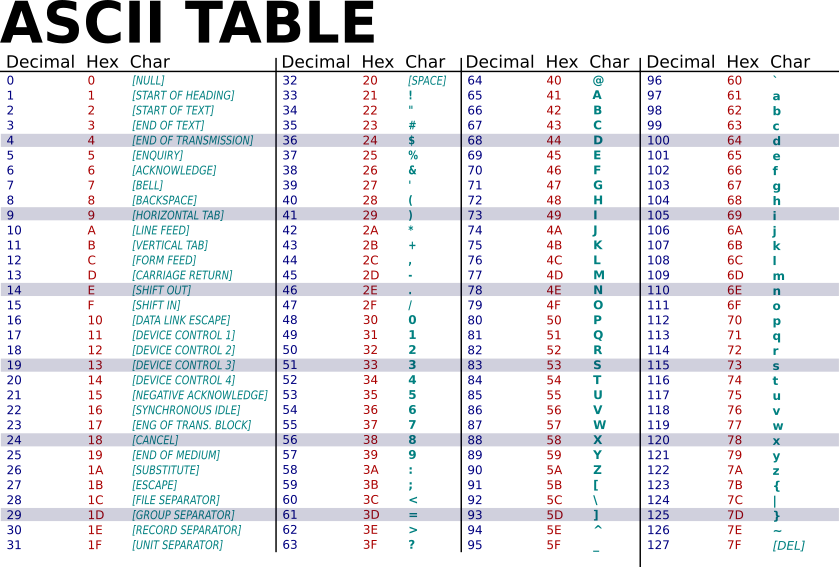
\includegraphics[width=.8\linewidth]{./gfx/ASCII_table}
	\caption[
		ASCII-Tabelle: Lookup-Tabelle zur Interpretation von Zahlen als Schriftzeichen
	]{
		ASCII-Tabelle: Lookup-Tabelle zur Interpretation von Zahlen als Schriftzeichen\\
		Quelle: \url{https://en.wikipedia.org/wiki/File:ASCII-Table-wide.svg}
	}
	\label{fig:ASCII}
\end{center}
\end{figure}

Wenn Sie sich diese Tabelle durchsehen, wird Ihnen auffallen, dass darin auch wieder Ziffern vorkommen. Das bedeutet, dass eine Zahl sowohl durch ihr Bitmuster dargestellt werden kann, als auch durch die Bitmuster ihrer Textdarstellung. Die Zahl \inPy{42} hat etwa das Bitmuster \texttt{00101010}. Als \emph{Text} \inPy{"42"} finden wir dagegen die Schriftzeichen \inPy{"4"} und \inPy{"2"} mit ASCII-Codes 52 und 50 und daher der das Bitmuster \texttt{00110110 00110100}. Genauso kann auch das Bitmuster \texttt{00101010} als das \emph{Schriftzeichen} mit der Nummer 42 gelesen werden, also als \inPy{"*"}.

Bisher mussten wir uns mit der Frage der Interpretation von Daten kaum beschäftigen, da jeder Ausdruck in Python einen zugeordneten \emph{Datentypen} hat; die Regeln zur Interpretation werden also \enquote{kostenlos} mitgeliefert. In Dateien dagegen können wir dagegen nur rohe Daten speichern. Als ProgrammiererInnen müssen wir uns also überlegen, wie und von wem diese Daten interpretiert werden sollen.

Wir unterscheiden im Wesentlichen zwischen \emph{Binärdaten} und \emph{Textdaten}. Binärdaten werden so auf die Festplatte geschrieben, wie sie auch im Speicher vorliegen, und auch so von dort gelesen. Man könnte sagen, Binärdaten seien die Muttersprache der Computer. Textdaten dagegen werden zuerst so übersetzt, dass sie ein menschlicher Leser leicht übersetzen kann.

In einem Beispiel: Sie haben im Speicher die \inPy{int}-Zahl \inPy{42}. Im Binärmodus wird daher das zugehörige Bitmuster \texttt{00101010} auf die Festplatte geschrieben. Öffnen wir diese Datei mit einem \emph{Text}editor, sehen wir das Zeichen \texttt{*}.\\
Wird dieselbe Zahl \inPy{42} dagegen im Textmodus geschrieben, so übersetzt Python diese zuerst in den \emph{Text} \inPy{"42"}, und schreibt dann diesen auf die Festplatte. Wir finden also das Bitmuster \texttt{00110110 00110100}. In einem Texteditor lesen wir auch wieder \texttt{42}.

Python erledigt all dieses Übersetzen für uns im Hintergrund. Wir als ProgrammiererInnen müssen aber zumindest vorgeben, ob eine Datei im Binärmodus oder im Textmodus gelesen/geschrieben werden soll.

\section{Einfacher Dateizugriff}
Python stellt \enquote{einfache Hausmittel} zur Arbeit mit Dateien zur Verfügung. Darauf aufbauend existieren weitere Module, die uns die Arbeit erleichtern, für die wir aber auch die \enquote{Hausmittel} im Prinzip verstanden haben müssen. 

\subsection{Dateien Öffnen und Schließen}
Um mit Dateien umzugehen, brauchen wir zunächst ein \emph{Handle auf die Datei}. Das ist eine Variable, in der alle nötigen Hintergrund-Informationen (Speicherort, Dateigröße, Netzwerkdatei oder lokale Datei, ...) zusammengefasst sind. Es handelt sich also um eine Klasseninstanz, deren Eigenschaften wir hier oberflächlich kennen lernen wollen. Stellen Sie sich das Handle tatsächlich als einen \enquote{Griff} vor, der an eine Datei angebracht wird: mit diesem Griff können Sie die Datei anpacken und darin Operationen (Lesen, Schreiben, Analysieren) durchführen.

Wir erhalten ein solches Handle über den Befehl \inPy{open}:
\begin{codebox}[Syntax: \texttt{open}]
\begin{minted}{python}
handle = open(Dateiname, Modus)
\end{minted}
\end{codebox}

Wie zu erwarten ist \texttt{Dateiname} ein String, der den Namen der Datei enthält, die geöffnet werden soll. Je nach Betriebssystem wird Groß- und Kleinschreibung unterschieden\footnote{Unter Windows wird nicht unterschieden. Linux und Mac dagegen erkennen \texttt{file} und \texttt{File} als unterschiedliche Dateien an.}. Die Datei wird im \emph{aktuellen Arbeitsverzeichnis} erwartet, \ie in dem Ordner, von dem aus Python auch gestartet wurde. Üblicherweise ist das derselbe Pfad, in dem auch Ihre Script-Datei liegt. Sollen Dateien in anderen Ordnern betrachtet werden, können aber auch \emph{absolute} und \emph{relative} Pfadangaben gemacht werden:

Absolute Pfadangaben enthalten die volle Information, wo im Dateisystem eine Datei abgelegt ist. Sie beginnt mit einem Betriebssystem-spezifischen Symbol für die \emph{Wurzel} des Dateisystems (\enquote{root}), und durch \emph{Forward Slashes /}\footnote{Unter Windows sind auch \emph{Backslashes} \textbackslash erlaubt und z.\;T. noch üblich. Dies bereitet aber oft Probleme mit Escape-Sequenzen und sollte daher vermieden werden} voneinander abgetrennte Ordnernamen. Unter Windows ist dieses Wurzel-Zeichen der \emph{Laufwerks-Buchstabe} gefolgt von einem Doppelpunkt. Ein gültiger Dateiname mit absoluter Pfadangabe unter Windows könnte also lauten:
\begin{center}
	\texttt{C:/User/some\_folder/myFile.txt}
\end{center}
Linux und Mac verwalten Laufwerke anders; die Wurzel des Dateisystems ist daher durch einen einfachen Forward Slash gekennzeichnet:
\begin{center}
	\texttt{/home/user/some\_folder/myFile.txt}
\end{center}

Relative Pfadangaben gehen vom aktuellen Arbeitsverzeichnis aus. Von diesem Startpunkt aus wird die Orderstruktur navigiert. Dass eine Pfadangabe relativ sein soll, wird erklärt, indem man als erstes Zeichen einen Punkt angibt.

Beispiel: Ihre Code-Datei liegt unter \texttt{/home/user/Codes/}. Die Datei, die Sie öffnen wollen, befindet sich in \texttt{/home/user/Codes/files}. In dem Fall können Sie auf diese Datei zugreifen, indem Sie als \inPy{Dateiname} angeben:
\begin{center}
	\texttt{./files/myFile.txt}
\end{center}
Dies gilt so gleichermaßen für Windows als auch für Linux und Mac.

Ist die Datei in einem \emph{Überordner}, so kann dies mit \emph{zwei Punkten} angezeigt werden. Wir können auch mehrere ebenen zurück gehen, indem wir Punkte und Slashes aneinander reihen: \texttt{../../} bezeichnet den Ordner \emph{zwei Ebenen} über dem Arbeitsverzeichnis. Weiter können wir diese Schreibweise auch mit relativen Pfadangaben kombinieren. Stellen wir uns wieder vor, das aktuelle Arbeitsverzeichnis wäre \texttt{/home/user/Codes/}. Die Datei, die Sie öffnen wollen, efindet sich nun aber im Order \texttt{/home/user/files}. In diesem Fall geben Sie an:
\begin{center}
	\texttt{../files/myFile.txt}
\end{center}


Unter \emph{Modus} verstehen wir, für welche Art Zugriff die Datei geöffnet werden soll. Wollen wir aus der Datei Lesen oder Schreiben? Soll der Zugriff im Text- oder Binärmodus stattfinden? Der Modus wird durch einen String beschrieben. Die wichtigsten Modi finden Sie in Tabelle \ref{tab:FileModes}:

\begin{center}
\rowcolors{1}{white}{tabhighlight}
\begin{tabular}{c|cp{.6\linewidth}}
	\toprule
	\textbf{String}	& \textbf{Bedeutung}				& \textbf{Kommentar} \tabcrlf
	\texttt{r}				& Lesen -- Textmodus				& Dateicursor am Anfang der Datei.\newline Neuen Dateien werden \emph{nicht} angelegt.\\
	\texttt{rb}			& Lesen -- Binärmodus			& Dateicursor am Anfang der Datei.\newline Neuen Dateien werden \emph{nicht} angelegt.\\
	\texttt{w}				& Schreiben -- Textmodus		& Dateicursor am Anfang der Datei.\newline Neuen Dateien werden angelegt, alte Dateien überschrieben.\\
	\texttt{wb}			& Schreiben -- Binärmodus	& Dateicursor am Anfang der Datei.\newline Neuen Dateien werden angelegt, alte Dateien überschrieben.\\
	\texttt{x}				& Schreiben -- Textmodus		& Dateicursor am Anfang der Datei.\newline Neuen Dateien werden angelegt, alte Dateien \emph{nicht} überschrieben.\\
	\texttt{xb}			& Schreiben -- Binärmodus	& Dateicursor am Anfang der Datei.\newline Neuen Dateien werden angelegt, alte Dateien \emph{nicht} überschrieben.\\
	\texttt{a}				& Anhängen -- Textmodus		& Dateicursor am \emph{Ende} der Datei. Neuen Dateien werden angelegt, alte Dateien \emph{nicht} überschrieben.\\
	\texttt{ab}			& Anhängen -- Binärmodus		& Dateicursor am \emph{Ende} der Datei. Neuen Dateien werden angelegt, alte Dateien \emph{nicht} überschrieben. \\
	\bottomrule
\end{tabular}
\captionof{table}{Dateimodi in Python}
\label{tab:FileModes}
\end{center}

\begin{hintbox}[Relative Pfadangaben bevorzugen]
Absolute Pfadangaben sind von Natur aus unflexibel. Wenn Sie Ihr Programm an Kollegen verschicken, wird es vermutlich nicht mehr funktionieren. Bevorzugen Sie daher relative Pfadangaben, und konzipieren Sie nach Möglichkeit Ihre Programme so, dass notwendige Dateien in \emph{Unterordnern} liegen.
\end{hintbox}

Jede Datei, die geöffnet wurde, sollte auch wieder geschlossen werden. Dies geschieht mit der Methode \inPy{close}:
\begin{codebox}[Syntax: \texttt{open}]
\begin{minted}{python}
handle.close()
\end{minted}
\end{codebox}

Ob eine Datei noch geöffnet ist, können wir mit dem Attribut \inPy{closed} in Erfahrung bringen: \inPy{handle.closed} ist entweder \inPy{True} oder \inPy{False}.

\subsection{Dateien Schreiben}
\subsubsection{Textmodus}
Sobald eine Datei in einem Text-Schreibmodus geöffnet wurde (\texttt{w},  \texttt{x} oder \texttt{a}), und solange sie noch nicht wieder geschlossen wurde, können wir mit der Methode \inPy{write} Text in eine Datei schreiben. Die Syntax ist denkbar einfach:

\begin{codebox}[Syntax: \texttt{write}]
\begin{minted}{python}
handle.write(Text)
\end{minted}
\end{codebox}

Dabei ist \inPy{Text} ein beliebiger Ausdruck, der zu einem String ausgewertet werden kann.

\begin{codebox}[Beispiel: Text-Dateien Schreiben]
\begin{minted}[linenos]{python}
handle = open("output.txt", "w")    # Text/Schreibmodus

handle.write("Some text\n")
handle.write("another line " * 2 + "\n")
handle.write( str(handle) )

handle.close()
\end{minted}
\end{codebox}

\begin{cmdbox}[Dateinhalt von \texttt{output.txt}]
\begin{minted}{text}
Some text
another line another line 
<_io.TextIOWrapper name='output.txt' mode='w' encoding='UTF-8'>
\end{minted}
\end{cmdbox}

Beachten Sie, dass, anders als bei \inPy{print} Zeilenumbrüche \emph{nicht} automatisch angehängt werden. Diese müssen explizit als \inPy{"\n"} teil des zu schreibenden Strings sein.

Im obigen Beispiel wird der \emph{Rückgabewert} der Methode ignoriert. \inPy{write} gibt die Zahl der in die Datei geschriebenen Bytes zurück. Dieses Feature wird selten gebraucht, kann aber unter Umständen nützlich sein.

Öffnen wir nach Zeile dieselbe Datei \texttt{output.txt} nochmals in den Modi \texttt{w}, \texttt{wb}, \texttt{x} oder \texttt{xb}, so wird der Dateiinhalt sofort gelöscht. Bei den Modi \texttt{a} und \texttt{ab} dagegen bleibt der alte Inhalt bestehen; neu geschriebener Text wird an das Ende der Datei angehängt.

\subsubsection{Binärmodus}
Schreiben im Binärmodus funktioniert prinzipiell genauso, wie wir es vom Textmodus schon kennen: Öffnen mit \inPy{open} in einem geeigneten Modus (\texttt{wb},  \texttt{xb} oder \texttt{ab}), Schreiben mit \inPy{handle.write(data)} und Schließen mit \inPy{handle.close()}. An das Objekt \inPy{data} muss \emph{eindeutig} in eine Byte-Sequenz übersetzt werden können. (Eingangs wurde gesagt, dass \eg der \inPy{int}-Wert \inPy{42} in das Bitpattern \texttt{00101010} übersetzt wird; gleichermaßen ist aber auch das Bitpattern \texttt{00000000 00101010} denkbar, und eine beliebige andere Zahl führender Nullen. Die Gründe hierfür sind leider etwas technisch, und können an dieser Stelle nicht erschöpfend erklärt werden).

Eine Klasse von Objekten, das eine solche absolut unmissverständliche Darstellung haben, sind Instanzen der Klasse \inPy{bytes}. Diese können beispielsweise aus \inPy{list}s erstellt werden, wenn deren einzelne Elemente nur Werte zwischen \inPy{0} und \inPy{255} annehmen.

\begin{codebox}[Beispiel: Binär-Dateien Schreiben]
\begin{minted}[linenos]{python}
handle = open("output.dat", "wb")    # Binär/Schreibmodus

data = bytes([65, 66, 67])
handle.write( data )

handle.close()
\end{minted}
\end{codebox}

\begin{cmdbox}[Dateinhalt von \texttt{output.dat}]
\begin{minted}{text}
ABC
\end{minted}
\end{cmdbox}


\subsection{Dateien Lesen}
Das Lesen aus Dateien gestaltet sich ähnlich einfach wie das Schreiben: nachdem die Datei in einem geeigneten Modus geöffnet wurde (\texttt{r} oder \texttt{rb}) kann mit den Methoden \inPy{read} und \inPy{readline} gearbeitet werden.

Beim Lesen können wir uns vorstellen, dass in der Datei ein \enquote{Cursor} platziert wird. Zu Beginn ist dieser ganz am Anfang der Datei. Mit jedem Lese-Befehl wandert dieser Cursor dann vorwärts. Gelesen wird immer jeweils von der aktuellen Cursorposition.

Die Methode \inPy{read} im einfachsten Fall \emph{die gesamte Datei} in den Arbeitsspeicher:
\begin{codebox}[Syntax: \texttt{read}]
\begin{minted}{python}
StringVariable = handle.read()
\end{minted}
\end{codebox}

Optional kann auch ein \inPy{int}-Parameter \inPy{size} mit übergeben werden. Dieser gibt eine Maximalmenge an Daten an, die aus der geöffneten Datei \inPy{handle} gelesen werden dürfen. 
\begin{codebox}[Syntax: \texttt{read} (erweitert)]
\begin{minted}{python}
StringVariable = handle.read(size)
\end{minted}
\end{codebox}
Dabei bezeichnet \inPy{size} die Zahl der Bytes, die maximal gelesen werden dürfen.

Die online-Dokumentation (\url{https://docs.python.org/3/tutorial/inputoutput.html}) kommentiert hierzu lakonisch:
\begin{center}
	\emph{It’s your problem if the file is twice as large as your machine’s memory.}
\end{center}

Beispiel: Wir wollen die im vorigen Abschnitt vorbereitete Datei \texttt{output.txt} zurück in den Arbeitsspeicher lesen. Dies erreichen wir mit dem folgenden Code:
\begin{codebox}[Beispiel: Text-Dateien Lesen]
\begin{minted}[linenos]{python}
handle = open("output.txt", "r")    # Text/Lesemodus

firstWord = handle.read(4)
rest      = handle.read()

handle.close()

print(firstWord)
print(rest)
\end{minted}
\end{codebox}

\begin{cmdbox}[Ausgabe: Text-Dateien Lesen]
\begin{minted}{text}
Some
 text
another line another line 
<_io.TextIOWrapper name='output.txt' mode='w' encoding='UTF-8'>
\end{minted}
\end{cmdbox}

Der Dateiinhalt wird als String in den Speicher geladen. Soll dieser wieder als Zahl behandelt werden, so muss der String mit den entsprechenden Funktionen (\inPy{int()}, \inPy{float()}, ...) umgewandelt werden.

Wird \enquote{nach dem Ende der Datei} versucht, weiter zu lesen, so ist das Ergebnis einfach ein leerer String.

Textdateien sollen besonders häufig Zeile für Zeile bearbeitet werden. Zu diesem Zweck existiert die Methode \inPy{readline}:
\begin{codebox}[Syntax: \texttt{readline}]
\begin{minted}{python}
StringVariable = handle.readline(size)
\end{minted}
\end{codebox}
\inPy{readline} liest von der aktuellen Cursorposition bis zum nächsten Zeilenumbruch. Wieder begrenzt der Parameter \inPy{size} die Datenmenge, die maximal gelesen wird. Wird dieser ausgelassen oder wird hier ein negativer Wert übergeben, so liest Python \emph{die gesamte Zeile}.

Verwandt mit der Methode \inPy{readline} ist die Methode \inPy{readlines}: Diese liest \emph{die gesamte Datei}, zerlegt sie dabei aber bereits an den Zeilenumbrüchen, und packt die Teilde der Datei in eine \inPy{list}:

\begin{codebox}[Beispiel: \texttt{readlines}]
\begin{minted}[linenos]{python}
handle = open("output.txt", "r")    # Text/Lesemodus

lines = handle.readlines()

handle.close()

for line in lines :
    print(line)
\end{minted}
\end{codebox}

Beachten Sie, dass die Zeilenumbrüche selbst beim Lesen nicht entfernt werden. Entsprechend sehen wir bei diesem Beispiel zusätzliche, leere Zeilen:

\begin{cmdbox}[Ausgabe: \texttt{readlines}]
\begin{minted}{text}
Some text

another line another line 

<_io.TextIOWrapper name='output.txt' mode='w' encoding='UTF-8'>
\end{minted}
\end{cmdbox}


\subsection{Dateien und Blockstrukturen}
hintbox -- with -- enter and exit


for line in handle

byteNum = handle.tell()
handle.seek(byteNum)

list(handle)

listOfLines = handle.readlines()

\section{JSON und pickle}


\section{PIL}

%	\chapter{Exceptions}
\label{chp:Exceptions}
\epigraph{
	With few exceptions, one ought always do what one is afraid of.
}{Viggo Mortensen}

Wie wir gesehen haben, bricht der Python-Interpreter die Ausführung unseres Codes ab, wenn sich die angeforderten Operationen als nicht Durchführbar herausstellen. Der Ausdruck \inPy{x / y} ist grundsätzlich ein sinnvolles Python-Codeelement, kann aber nicht ausgewertet werden, wenn \texttt{y} den Wert 0 hat. In diesem Fall wird eine sogenannte \emph{Ausnahme} (\emph{Exception}) ausgelöst. Unser Ziel als ProgrammiererIn sollte es sein, solche Ausnahmen zu vermeiden. Manchmal ist es aber bequemer, im Nachgang auf Fehler zu reagieren, als diese bereits im Vorfeld abzufangen. Dieses Kapitel soll Ihnen zeigen, wie Sie in Ihre Codes Fehlerbehandlung einbauen.

\section{\inPy{try-except}-Blocks}
\subsection{Grundlegendes}
Eine \emph{Ausnahme} ist eine Instanz einer Klasse, die Informationen zum letzten Laufzeitfehler enthält. Tritt ein Fehler in der Codeausführung auf, so wird eine Instanz dieser Klasse angelegt, und durch verschiedene Routinen durchgereicht. Ultimativ wird sie in einem Kernmodul des Python-Interpreters landen, der auf dieses Signal hin die Ausführung unterbricht -- es sei denn, wir schreiben Code, der diese Instanz abfängt und nicht mehr weiterreicht. Genau zu diesem Zweck existieren \inPy{try-except}-Blocks.

\inPy{try-except}-Blocks bestehen aus einem \inPy{try}-Block, in dem Anweisungen stehen, die potentiell einen Fehler erzeugen könnten, sowie (mindestens) einem \inPy{except}-Block, in den beschrieben wird, was geschehen soll, wenn dieser Fehler auftritt:

\begin{codebox}[Syntax: \texttt{try-except}]
\begin{minted}{python}
try :
    Code der eine Ausnahme auslösen könnte
except ExceptionClass as varible :
    Code zur Fehlerbehandlung
\end{minted}
\end{codebox}

Mit \texttt{ExceptionClass} ist dabei die \enquote{Art der Ausnahme} gemeint, also die Fehlerklasse, die Sie sonst bei Programmabbruch angezeigt bekämen:

\begin{cmdbox}[Auslösen einer Exception und Anzeige in der Python-Konsole]
\begin{minted}{text}
>>> print(1/0)
Traceback (most recent call last):
  File "<stdin>", line 1, in <module>
ZeroDivisionError: division by zero
\end{minted}
\end{cmdbox}

Die letzte Zeile der Fehlermeldung zeichnet die aufgetretene Ausnahme also als \texttt{ZeroDivisionError} aus. Eben dies sollte auch anstelle von \texttt{ExceptionClass} in einer entsprechenden \inPy{except}-Zeile stehen.

\texttt{variable} ist eine neue Variable, mit der wir auf die Daten der Instanz von \texttt{ExceptionClass} zugreifen können.

Tritt während der Ausführung des \inPy{try}-Blocks eine Ausnahme der Klasse \texttt{ExceptionClass} auf, so wird der Code des entsprechenden \inPy{except}-Blocks ausgeführt; danach setzt Python die Ausführung mit \emph{der ersten Zeile nach dem \inPy{try-except}-Block fort}.

\begin{codebox}[Beispiel: Inverse]
\begin{minted}[linenos]{python}
for x in range(-3, 3) :
    try :
        print(1/x)
    except ZeroDivisionError as e :
        print("An exception was caught:", e)
\end{minted}
\end{codebox}

\begin{cmdbox}[Ausgabe: Inverse]
\begin{minted}{text}
-0.3333333333333333
-0.5
-1.0
An exception was caught: division by zero
1.0
0.5
\end{minted}
\end{cmdbox}

Beachten Sie auch, dass es durchaus von Bedeutung ist, welche Strukturen Sie wie ineinander schachteln: Vertauschen Sie im obigen Beispiel den \inPy{for}- mit dem \inPy{try}-Block, so werden die Inversen der positiven Zahlen nicht mehr berechnet:

\begin{codebox}[Beispiel: Inverse II]
\begin{minted}[linenos]{python}
try :
    for x in range(-3, 3) :
        print(1/x)
except ZeroDivisionError as e :
    print("An exception was caught:", e)
\end{minted}
\end{codebox}

\begin{cmdbox}[Ausgabe: Inverse II]
\begin{minted}{text}
-0.3333333333333333
-0.5
-1.0
An exception was caught: division by zero
\end{minted}
\end{cmdbox}

Ist der aufgetretene Fehler nicht in der Klasse, die im \inPy{except}-Block genannt wurde, so ignoriert Python die bereitgestellte Fehlerbehandlung und bricht wie üblich die Fehlerbehandlung ab:

\begin{codebox}[Beispiel: Fehlerklassen]
\begin{minted}[linenos]{python}
import math
try :
    print( math.log(-1) )
except ZeroDivisionError as e :
    print("An exception was caught:", e)
\end{minted}
\end{codebox}

\begin{cmdbox}[Ausgabe: Fehlerklassen]
\begin{minted}{text}
Traceback (most recent call last):
  File "<stdin>", line 3, in <module>
ValueError: math domain error
\end{minted}
\end{cmdbox}

Ausnahmen haben eine hierarchische Struktur, \ie manche Ausnahmen sind Spezialisierungen von anderen. So ist beispielsweise \texttt{ZeroDivisionError} eine Abwandlung von \texttt{ArithmeticError}. In Beispiel: Inverse und Inverse II würden also genauso funktionieren, wenn Zeile 4 jeweils durch \inPy{except ArithmeticError as e :} ausgetauscht würde. Die allgemeinste (sinnvoll verwendbare) Fehlerklasse ist \texttt{Exception}. Im Kasten \emph{Ausgewählte Fehlerklassen} finden Sie eine Aufzählung häufig ausgelöster Ausnahmen.

\begin{figure}
\begin{tcolorbox}[title=Ausgewählte Fehlerklassen]
 \renewcommand{\labelitemi}{\textbullet}
 \renewcommand{\labelitemii}{\textendash}
 \renewcommand{\labelitemiii}{\textperiodcentered}
\begin{itemize}
\item \texttt{Exception} (Generelle Fehlermeldung)
	\begin{itemize}
	\item \texttt{StopIteration} (Wird von \emph{iterierbaren} Objekten ausgelöst, um \inPy{for}-Schleifen mitzuteilen, dass sie fertig durchlaufen sind.)
  \item \texttt{ArithmeticError} (Fehler bei Berechnungen)
	  		\begin{itemize}
	  		\item \texttt{FloatingPointError} (Fehler spezifisch für Fließkommaberechnungen)
	    \item \texttt{OverflowError} (Ergebnis zu groß für den bereitgestellten Speicher)
	    \item \texttt{ZeroDivisionError} (Division durch Null)
  			\end{itemize}
    \item \texttt{EOFError} (Lesezugriff nach Dateiende) (EOF: End of File)
    \item \texttt{ImportError} (Fehler bei Bearbeitung einer \inPy{import}-Zeile)
    		\begin{itemize}
    		\item \texttt{ModuleNotFoundError} (Angegebenes Modul wurde nicht gefunden)
    		\end{itemize}
    	\item \texttt{LookupError} (Fehler bei Zugriff auf ein Container-Element)
    		\begin{itemize}
    		\item \texttt{IndexError} (Ungültiger Index)
			\item \texttt{KeyError} (Ungültiger Schlüssel bei \inPy{dict}s)
    		\end{itemize}
		\item \texttt{NameError} (Symbol mit diesem Namen existiert nicht)
		\item \texttt{OSError} (Fehler bei Nutzung von Funktionen des Betriebssystems)
			\begin{itemize}
			\item \texttt{FileExistsError} (Datei existiert bereits)
      \item \texttt{FileNotFoundError} (Datei kann nicht gefunden werden)
			\end{itemize}
		\item \texttt{RuntimeError}
			\begin{itemize}
			\item \texttt{NotImplementedError} (Methode/Variante einer Methode einer Klasse wurde nicht implementiert)
      \item \texttt{RecursionError}
			\end{itemize}
		\item \texttt{SyntaxError}
			\begin{itemize}
			\item \texttt{IndentationError}
			\end{itemize}
		\item \texttt{TypeError} (Datentyp kann nicht verarbeitet werden)
		\item \texttt{ValueError} (Unzulässiger Wert bei Funktionsaufruf)
	\end{itemize}
\end{itemize}
Siehe \url{https://docs.python.org/3/library/exceptions.html} für weitere Details.
\end{tcolorbox}
\end{figure}


\subsection{Mehrteilige \inPy{except}-Blöcke}
Hinter \inPy{except} darf auch ein \inPy{tuple} von Fehlerklassen stehen, die dann jeweils mit demselben Code behandelt werden. Wir können also beispielsweise schreiben:
\begin{codebox}[Syntax: \texttt{tuple} von Fehlerklassen]
\begin{minted}{python}
except (ZeroDivisionError, ValueError) as e :
\end{minted}
\end{codebox}
Wenn ein Fehler auftritt, der auf wenigstens eine der Klassen im \inPy{tuple} passt (im Beispiel also entweder ein \inPy{ZeroDivisionError} oder ein \inPy{ValueError}), betritt der Python-Interpreter die \inPy{except}-Umgebung und setzt nach dieser die Ausführung am Ende des \inPy{try-except}-Blocks fort.

Daneben ist es auch möglich, mehrere \inPy{except}-Blöcke hintereinander zu setzen, und für jede Fehlerklasse einen eigenen Code zur Fehlerbehandlung zu schreiben. Dabei wird nur der \emph{erste \inPy{except}-Block} abgearbeitet, der zur ausgelösten Ausnahme passt.

\begin{codebox}[Beispiel: Mehrere \texttt{except}-Blöcke]
\begin{minted}[linenos]{python}
try :
    print(1/0)
except ArithmeticError as e :
    print("Arithmetic Unit Error")
except ZeroDivisionError as e :
    print("Division by Zero.")
\end{minted}
\end{codebox}

\begin{cmdbox}[Ausgabe: Mehrere \texttt{except}-Blöcke]
\begin{minted}{text}
Arithmetic Unit Error
\end{minted}
\end{cmdbox}

Der Ausdruck \inPy{1/0} löst bekanntermaßen die Ausnahme \texttt{ZeroDivisionError} aus; diese ist jedoch eine Spezialisierung von \texttt{ArithmeticError}, welche im obigen Beispiel zuerst bearbeitet wird. Die Behandlung von \texttt{ZeroDivisionError} findet also unter keinen Umständen statt.

\subsection{\inPy{else} und \inPy{finally}}
Soll Code nur ausgeführt werden, wenn im \inPy{try}-Block \emph{kein} Fehler aufgetreten ist, so kann dies mit einem \inPy{else}-Block erreicht werden. Dieser Block steht hinter den \inPy{except}-Blöcken und wird ausgeführt, nachdem die Behandlung des \inPy{try}-Blocks abgeschlossen wurde.

Das Schlüsselwort \inPy{finally} leitet einen weiteren Block ein, in dem Code steht, der ausgeführt wird, nachdem alle \inPy{except}- und \inPy{else}-Blöcke bearbeitet wurden, selbst wenn der tatsächlich eingetretene Fehler noch nicht abgefangen wurde:

\begin{codebox}[Beispiel: Mehrere \texttt{try-except-else-finally}]
\begin{minted}[linenos]{python}
def divide(x, y):
    try:
        result = x / y
    except ZeroDivisionError:
        print("division by zero!")
    else:
        print("result is", result)
    finally:
        print("executing finally clause")

print("divide(2, 1)")
divide(2, 1)
print()

print("divide(2, 0)")
divide(2, 0)
print()

print('divide("2", "0")')
divide("2", "1")
\end{minted}
\end{codebox}

\begin{cmdbox}[Ausgabe: Mehrere \texttt{except}-Blöcke]
\begin{minted}{text}
divide(2, 1)
result is 2.0
executing finally clause

divide(2, 0)
division by zero!
executing finally clause

divide("2", "1")
executing finally clause
Traceback (most recent call last):
  File "<stdin>", line 1, in <module>
  File "<stdin>", line 3, in divide
TypeError: unsupported operand type(s) for /: 'str' and 'str'
\end{minted}
\end{cmdbox}



\subsection{\inPy{raise}}
In Kapitel \ref{chp:Classes} (Klassen) haben wir bereits gesehen, dass wir mit dem Befehl \inPy{raise} die Fehlerbehandlung auslösen können: Nach \inPy{raise} können wir eine Fehlerklasse (\eg ValueError) nennen. Eine Instanz dieser Fehlerklasse wird dann angelegt und ruft das oben beschriebene Verhalten aus:
\begin{itemize}
\item Unbehandelt bricht der Python-Interpreter die Code-Ausführung ab und gibt eine Fehlermeldung aus
\item In einem \emph{passenden} \inPy{except}-Block kann der Fehler \enquote{aufgefangen} und behandelt werden.
\end{itemize}
In der Regel erlauben die Fehlerklassen, ihrem Konstruktor noch ein String-Argument mitzugeben, in dem dann der aufgetretene Fehler in für Menschen lesbarer Form genauer beschrieben wird. In einem früheren Beispiel finden Sie etwa die Zeile
\begin{codebox}[Beispiel: Auszug aus einem früheren Code]
\begin{minted}{python}
raise Exception("Incompatible Shapes")
\end{minted}
\end{codebox}

Diese Zeile löst also eine Ausnahme vom Typ \inPy{exception} aus. Die Zusatzinformation \inPy{"Incompatible Shapes"} wird der Ausnahme angehängt und taucht auf, wenn Informationen zum aufgetretenen Fehler ausgegeben werden sollen.

\begin{hintbox}[Fehlerklassen möglichst spezifisch wählen]
Die Klasse \inPy{Exception} ist die allgemeinste Fehlerklasse. \emph{Alle} auftretenden Fehler werden über \inPy{except Exceptoin as e :} abgefangen. Die Behandlung von verschiedenen Arten von Fehlern kann sehr verschiedenartig sein. In manchen Fällen wollen Sie vielleicht nur eine Warnung auf dem Bildschirm ausgeben, während andere Fehlerklassen eine Datei bearbeiten sollten oder ein extern angeschlossenes Gerät ausschalten müssen.

Damit Sie ihren Fehlerbehandlungs-Code richtig schreiben können und nicht in unerwarteten Situationen auslösen, sollten Sie auch geeignete, \emph{spezifische} Fehlerklassen wählen. Vermeiden Sie daher \inPy{raise Exception} bzw. \inPy{except Exceptoin as e :} und benutzen Sie stattdessen lieber Fehlerklassen wie \inPy{ZeroDivisionError}.
\end{hintbox}

Ausnahmen können auch nach der Behandlung \enquote{neu aufgelegt} werden. Wollen Sie beispielsweise eine detaillierte Fehlerbeschreibung ausgeben, aber dennoch das Programmende auslösen, so erreichen Sie dies, indem Sie im \inPy{except}-Block erneut \inPy{raise} (ohne weitere Argumente) schreiben:

\begin{codebox}[Beispiel: Re-\texttt{raise}]
\begin{minted}[linenos]{python}
try :
    x = 7
    y = 0
    print(x / y)
except ZeroDivisionError as e :
    print("Division durch 0 aufgetreten!")
    print("Fehlerbeschreibung: ", e)
    print("x =", x)
    print("y =", y)
    raise

print("Wird nie ausgeführt.")
\end{minted}
\end{codebox}

\begin{cmdbox}[Ausgabe: Re-\texttt{raise}]
\begin{minted}{text}
Division durch 0 aufgetreten!
Fehlerbeschreibung:  division by zero
x = 7
y = 0
Traceback (most recent call last):
  File "<stdin>", line 4, in <module>
ZeroDivisionError: division by zero

\end{minted}
\end{cmdbox}

Wie Sie sehen, nennt die Ausgabe immer noch Zeile 4 als Punkt, an dem die Ausnahme ausgelöst wurde. Würden wir in Zeile 10 statt einem einfachen \inPy{raise} den Ausdruck \inPy{raise ZeroDivisionError}, so würde die Ausgabe auch Zeile 10 als Auslöser der Ausnahme melden.

Ein solches re-raise verlässt den gesamten \inPy{try}-Block. Auch nachgelagerte, passende \inPy{except}-Blocks werden ignoriert. Ein äußerer \inPy{try}-Block dagegen kann die re-raised Ausnahme dagegen immer noch auffangen:
\begin{codebox}[Beispiel: Re-\texttt{raise}]
\begin{minted}[linenos]{python}
try :
    try :
        print(1/0)
    except ArithmeticError as e :
        print("Arithmetic Unit Error")
        raise   # leaves entire structure
    except ZeroDivisionError as e :
        print("Innerer Block wird übersprungen.")
except ZeroDivisionError as e :
    print("Äußerer Block wird behandelt")
\end{minted}
\end{codebox}

\begin{cmdbox}[Ausgabe: Re-\texttt{raise}]
\begin{minted}{text}
Arithmetic Unit Error
Äußerer Block wird behandelt
\end{minted}
\end{cmdbox}

Zeile 3 löst bekanntermaßen einen \inPy{ZeroDivisionError} aus. Dieser ist eine spezielle Form eines \inPy{ArithmeticError}s, und löst somit die Fehlerbehandlung in Zeile 4 aus (und damit die Ausgabe \texttt{Arithmetic Unit Error}). Das \inPy{raise} in Zeile 5 dann markiert den Fehler als noch nicht vollständig bearbeitet und verlässt den gesamten \inPy{try}-Block, der in Zeile 2 begonnen hat. Auch \inPy{except ZeroDivisionError} in Zeile 7 kommt damit nicht mehr in Frage.

Dagegen findet die Fehlerbehandlung jetzt eine Ebene höher statt, \ie in dem \inPy{try}-Block, der in Zeile 1 begonnen hat. Damit wird also die Fehlerbehandlung in Zeile 9 ausgelöst, und wir finden eine zweite Meldung \texttt{Äußerer Block wird behandelt} auf dem Bildschirm.

\section{Eigene Ausnahmen}
Wir sollten Ausnahmen immer so spezifisch wie möglich aufwerfen. Die vorgefertigten Ausnahmen, die mit dem Standardumfang der Sprache Python angeboten werden, sind aber nicht besonders zahlreich und können unmöglich alle erdenklichen Szenarios abdecken, die wir als fehlerhaft behandeln wollen könnten. Wir müssen also auch eigene Fehlerklassen erstellen können.

Dies Geschieht nach dem Formalismus von von Klassen, wie wir ihn in Kapitel \ref{chp:Classes} bereits kennengelernt haben. Ausnahmen sind damit einfach von \inPy{Exception} abgeleitete Klassen.

Beispiel: Wir wollen fehlerhafte User-Eingaben als eigene Fehlerklasse abbilden. Dazu legen wir eine neue Klasse \inPy{UserInputError} an, die wir von \inPy{Exception} ableiten:

\begin{codebox}[Beispiel: Eigene Fehlerklasse anlegen]
\begin{minted}[linenos]{python}
class UserInputError(Exception) :
    pass

try:
    x = float(input("Bitte eine positive Zahl eingeben"))
    if x < 0 :
        raise UserInputError("Zahl war negativ!")
except UserInputError as e :
    print(e)
    
\end{minted}
\end{codebox}

Die Klasse \inPy{UserInputError} erbt alle Eigenschaften von \inPy{Exception} und ist damit effektiv eine Kopie von \inPy{Exception} mit neuem Namen. Wir müssen mindestens eine Code-Zeile in der Block-Anweisung \inPy{class} schreiben; daher setzen wir hier in \inPy{pass}, das keine weitere Auswirkung hat, aber die Anforderung an die Syntax erfüllt (keine leeren Block-Anweisungen).

Mit dieser neuen Klasse können wir jetzt also alle Techniken anwenden, die wir oben bereits besprochen hatten.

Natürlich können Sie Ihre Fehlerklassen auch weiter ausgestalten, und eigene Attribute und Methoden hinzufügen. Beim \inPy{raise} wird ein von Ihnen frei gestaltbarer Konstruktor aufgerufen (\ie die Methode \inPy{__init__}), was es Ihnen erlaubt, zusätzliche Informationen an die Fehlerbehandlung zu übertragen. Als Minimalbeispiel reicht aber bereits der oben gezeigte Code.

Selbstverständlich können Sie auch ihre eigenen Fehlerklassen als Basisklassen verwenden. Das bedeutet, dass eine weitere Klasse \inPy{UserInputNumericError} von der bereits beschriebenen Klasse \inPy{UserInputError} erben könnte. Damit erzeugen Sie genau eine solche hierarchische Struktur, wie sie im Infokasten \emph{Ausgewählte Fehlerklassen} bereits beschrieben ist.
%	\chapter{Grafische Darstellung von Daten -- Die MatPlotLib}
\label{chp:Matplotlib}
\epigraph{
	Real life seems to have no plots.
}{Ivy Compton-Burnett}

Menschen sind unheimlich gut darin, Bilder zu interpretieren. Computer haben ihre Stärke in der Auswertung von rohen Zahlen. Um nun die Früchte unserer Datenverarbeitung mit Python zu ernten, wollen wir Daten als graphische Plots ausgeben. Ein einfach zu bedienendes Mittel hierzu ist die MatPlotLib bzw. das Untermodul PyPlot. Das Modul MatPlotLib bietet tatsächlich so viele Funktionen, dass damit ein eigenständiger Kurs gefüllt werden könnte. Hier soll Ihnen eine Basis gezeigt werden, mit der Sie die häufigsten Aufgaben lösen können, und auf der Sie im Selbststudium leicht aufbauen können.

Eine erste Übersicht über die Funktionen der MatPlotLib finden Sie auch unter \url{https://matplotlib.org/tutorials/introductory/pyplot.html}.

\section{Grundlagen}
An dieser Stelle möchte ich Ihnen zuerst einen einfachen Code zeigen, und diesen dann Zeile für Zeile \enquote{entziffern}:

\begin{codebox}[Beispiel: Einfacher Plot, width=.55\linewidth, nobeforeafter, equal height group = grpXmpSimplePlot]
\begin{minted}[linenos]{python3}
import math
import matplotlib.pyplot as plt

N = 100
X = [(x - N/2) / 10 for x in range(N)]
Y = [math.sin(x) for x in X]

plt.plot(X, Y)
plt.show()
\end{minted}
\end{codebox}
%
\begin{tcolorbox}[title=Ausgabe: Einfacher Plot, width=.45\linewidth, nobeforeafter, equal height group = grpXmpSimplePlot]
	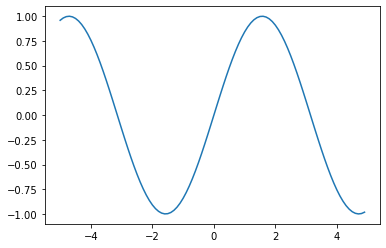
\includegraphics[width=\linewidth]{./gfx/plt-sin}
	\captionof{figure}{Einfacher Plot der matplotlib}
\end{tcolorbox}

In den Zeilen 1 und 2 laden wir Module -- zum einen das Modul \inPy{math}, mit dem wir die Daten generieren, die auf unserem Plot erscheinen sollen, und zum anderen die Matplotlib. Tatsächlich handelt es sich dabei um ein extrem umfangreiches Paket, weswegen wir nur einen Teil davon in unser Projekt integrieren: Das Untermodul \inPy{pyplot}\footnote{Die Matplotlib enthält Code zum Fenstermanagement, zur Interpolation von Kurven, Umgang mit Dateien, ... Alle diese Features bilden den Unterbau von \inPy{pyplot}, müssen aber nicht \enquote{offengelegt} werden, um für uns nützlich zu sein. Während \inPy{pyplot} intern alle diese Objekte und Funktionen benutzt und korrekt verwaltet, können wir uns auf das \emph{Interface} konzentrieren, das uns \inPy{pyplot} auf all diese Features bietet.}. Da dieser Modulname \inPy{matplotlib.pyplot} eher unhandlich ist, hat es sich eingebürgert, \inPy{plt} als Kurzname hierfür zu verwenden.

In den kommenden drei Zeilen generieren wir Werte, die schließlich geplottet werden sollen. \inPy{X} und \inPy{Y} sind jeweils Listen mit \inPy{N = 100} Elementen. Die Werte in \inPy{X} sind einfach gleichverteilte Werte im Abstand von \texttt{0.1}, rund um die \texttt{0} herum. Die Werte in \inPy{Y} enthalten jeweils den Sinus dieser \inPy{X}-Werte. Bis hierhin also haben wir noch nichts Neues gesehen.

In Zeile 8 wird nun die Funktion \inPy{plot} aus dem Modul \inPy{plt} aufgerufen. Diese Funktion bereitet alles vor, das nötig ist, um einen Plot zu generieren: Ein Arbeitsfenster, Achsen mit Beschriftung, Datenpunkte in den Graphen eintragen, ... All das wird aber nur im Arbeitsspeicher vorbereitet, jedoch noch nicht sichtbar gemacht. Grund hierfür ist, dass wir die Standard-Einstellungen noch abändern könnten: eine andere Linienfarbe, Skalierung, Bemaßung, \ldots Wenn jede Änderung in Echtzeit auf dem Bildschirm umgesetzt würde, hätte dies ein unangenehmes Flackern zur Folge, bevor der Plot endlich fertig aufgebaut ist. Stattdessen müssen wir manuell festlegen, wann unser Plot fertig beschrieben ist, \ie wann er auf dem Bildschirm erscheinen soll. Dies geschieht in Zeile 10.

Im einfachsten Fall müssen wir also folgende Arbeitsschritte erledigen:
\begin{itemize}
\item Das Modul \texttt{matplotlib.pyplot} laden
\item X- und Y-Werte als getrennte Listen vorbereiten
\item Die Funktion \texttt{plot} aufrufen
\item Die Funktion \texttt{show} aufrufen
\end{itemize}

Tatsächlich ist das Vorbereiten von X-Werten \emph{streng genommen} sogar überflüssig:

\begin{codebox}[Beispiel: Einfacher Plot ohne X-Werte, width=.55\linewidth, nobeforeafter, equal height group = grpXmpSimplePlotSansX]
\begin{minted}[linenos]{python3}
import matplotlib.pyplot as plt

N = 100
Y = [(x - 50) * x for x in range(N)]

plt.plot(Y)
plt.show()
\end{minted}
\end{codebox}
%
\begin{tcolorbox}[title=Ausgabe: Einfacher Plot ohne X-Werte, width=.45\linewidth, nobeforeafter, equal height group = grpXmpSimplePlotSansX]
	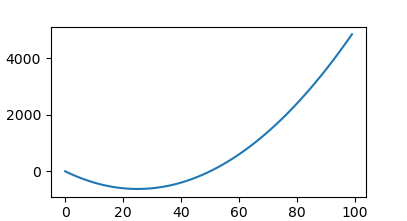
\includegraphics[width=\linewidth]{./gfx/plt-square}
	\captionof{figure}{Einfacher Plot ohne explizite x-Werte}
\end{tcolorbox}

Wenn keine X-Werte angegeben werden, erhalten wir zwar einen \enquote{sinnvollen} Plot; Python hat jedoch natürlich keine Möglichkeit, zu entscheiden, welcher Wert an welche Position gehört. Daher geht der Plotter hier davon aus, dass die Werte bei \inPy{x=0} beginnen und jeweils einen Abstand von \inPy{1} zueinander haben.

Folgen zwei \texttt{plot()}-Befehle direkt aufeinander ohne ein \texttt{show()} dazwischen, so werden beide Graphen auf denselben Plot gezeichnet. Jeder Plot bekommt dabei seine eigene Farbe. Eine Legende wird jedoch nicht \emph{automatisch} angezeigt.

\begin{codebox}[Beispiel: Zwei Graphen im selben Plot, width=.55\linewidth, nobeforeafter, equal height group = grpXmpSimplePlotTwoFunc]
\begin{minted}[linenos]{python3}
import matplotlib.pyplot as plt

N = 100
W = 10
X = [(x - N/2) / W for x in range(N)]
Y = [(x - W/2) * x for x in X]

plt.plot(X, Y)
plt.plot(X, [2 * y for y in Y])

plt.show()
\end{minted}
\end{codebox}
%
\begin{tcolorbox}[title=Ausgabe: Zwei Graphen im selben Plot, width=.45\linewidth, nobeforeafter, equal height group = grpXmpSimplePlotTwoFunc]
	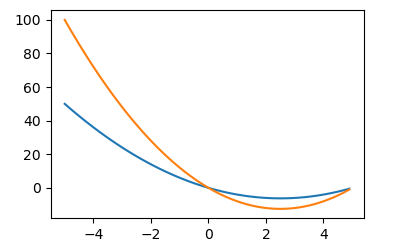
\includegraphics[width=\linewidth]{./gfx/plt-twoFuncs}
	\captionof{figure}{Zwei Graphen}
\end{tcolorbox}

\section{Einfache Formatierungen und andere Plot-Arten}
\subsection{Format-Angaben im Befehl \texttt{plot}}
Es wurde schon angesprochen, dass die Standard-Einstellungen der MatPlotLib nicht übernommen werden müssen. Im einfachsten Fall können wir direkt im \texttt{plot}-Befehl eine andere Linienfarbe und -form festlegen: Nach den Y-Werten kann ein optionaler String übergeben werden, in dem diese Information enthalten ist:
\mint{python3}{plt.plot(X, Y, "r--")}
weist die MatPlotLib dazu an, den Plot in Rot mit Strichlinien zu zeichnen. Dagegen steht
\mint{python3}{plt.plot(X, Y, "b-.")}
für einen Graphen aus blauen Punkten, die durch mit einer Linie verbunden sind. Folgende Zeichen werden verstanden und können auch miteinander kombiniert werden:

\begin{tcolorbox}[title=Format-Strings für \texttt{plt.plot()}]
\textbf{Punktarten}
\vspace{-6pt}
\begin{center}
	\begin{tabular}{cc|cc|cc}
		Symbol     & Punkt         & Symbol                    & Punkt            & Symbol     & Punkt            \tabcrlf
		\texttt{,} & Pixel         & \texttt{.}                & kleiner Punkt    & \texttt{o} & großer Punkt     \\
		\texttt{s} & Quadrat       & \texttt{d}                & schmale Raute    & \texttt{D} & breite Raute     \\
		\texttt{p} & Fünfeck       & \texttt{h}                & Sechseck stehend & \texttt{H} & Sechseck liegend \\
		\texttt{|} & Strich        & \texttt{+}                & Plus             & \texttt{x} & Kreuz            \\
		\texttt{<} & Dreieck links & \texttt{>}                & Dreieck rechts   & \texttt{*} & Stern            \\
		\texttt{v} & Dreieck unten & \texttt{\textasciicircum} & Dreieck oben                                     \\
	\end{tabular}
\end{center}

\textbf{Linienarten}
\vspace{-15pt}
\begin{center}
	\begin{tabular}{cc|cc|cc|cc}
		Symbol     & Linie        & Symbol      & Linie       & Symbol     & Linie     & Symbol      & Linie       \tabcrlf
		\texttt{-} & durchgezogen & \texttt{--} & gestrichelt & \texttt{:} & gepunktet & \texttt{-.} & strichpunkt \\
	\end{tabular}
\end{center}
\end{tcolorbox}
%
\begin{tcolorbox}
\textbf{Farben}
\begin{center}
	\begin{tabular}{cc|cc|cc|cc}
		Symbol     & Farbe   & Symbol     & Farbe   & Symbol     & Farbe & Symbol     & Farbe  \tabcrlf
		\texttt{b} & blau    & \texttt{c} & cyan    & \texttt{g} & grün  & \texttt{k} & schwarz \\
		\texttt{m} & magenta & \texttt{r} & rot     & \texttt{y} & gelb  & \texttt{w} & weiß    \\
	\end{tabular}
\end{center}

\captionof{table}{Formatstring-Elemente für \texttt{plot}}
\label{tab:PlotFormatStrings}
\end{tcolorbox}

Soll eine Kurve in einer Farbe gezeichnet werden, die nicht in Tabelle \ref{tab:PlotFormatStrings} aufgeführt sind, kann das Keyword-Argument \texttt{color} verwendet werden. Hier gibt man die Farbe als RGBA-String mit führendem Raute-Symbol an. Das bedeutet, dass der Rot- Grün- und Blau-Anteil der Farbe sowie die Deckkraft (\enquote{Alpha-Wert}) als zweistellige Hexadezimalzahl geschrieben wird und diese vier Zahlen dann aneinander gereiht werden. Für ein dunkles Rot kann man also schreiben:
\mint{python3}{plt.plot(X, Y, color="#7F0000FF")}
Dabei ist \inPy{7F} der Rot-Anteil (entspricht 50\% Intensität), \inPy{00} jeweils der Grün- und Blau-Anteil und \inPy{FF} die Deckkraft (entspricht 100\%).

\subsection{Legenden Anzeigen und Gitter anzeigen -- \texttt{legend}, \texttt{label} und \texttt{grid}}
Weiter ist es natürlich auch möglich, Graphen zu benennen und eine Legende anzeigen zu lassen. Dazu sind zwei Dinge nötig:
\begin{itemize}
\item Im Plot-Befehl muss mit dem Keyword-Argument \texttt{label} ein Titel angegeben werden
\item Mit dem Befehl \texttt{legend()} muss die Legende auch angezeigt werden:
\end{itemize}

\begin{codebox}[Beispiel: Plot mit Legende, width=.55\linewidth, nobeforeafter, equal height group = grpXmpSimplePlotLegend]
\begin{minted}[linenos]{python3}
import math
import matplotlib.pyplot as plt

N  = 100
X  = [(x - N/2) / 10 for x in range(N)]
Y1 = [math.sin(x) for x in X]
Y2 = [math.cos(x) for x in X]

plt.plot(X, Y1, label="Sinus")
plt.plot(X, Y2, label="Cosinus")

plt.legend()
plt.show()
\end{minted}
\end{codebox}
%
\begin{tcolorbox}[title=Ausgabe: Plot mit Legende, width=.45\linewidth, nobeforeafter, equal height group = grpXmpSimplePlotLegend]
	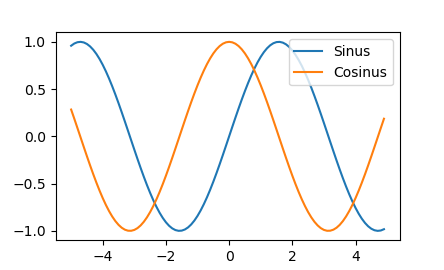
\includegraphics[width=\linewidth]{./gfx/plt-legend}
	\captionof{figure}{Plot mit Legende}
\end{tcolorbox}

Dem Befehl \texttt{plot} können noch viele weitere Keyword-Arguments mitgegeben werden, auf die hier nicht weiter eingegangen werden kann. Sie können sich bei Bedarf selbst die Bedeutung und Anwendung dieser Schlüsselworte anlesen; siehe hierzu die Dokumentation unter 
\url{https://matplotlib.org/2.1.2/api/_as_gen/matplotlib.pyplot.plot.html}

Um die Werte aus dem Plot besser ablesbar zu machen können auch Hilfslinien dazugeschalten werden. Dies erreicht der Befehl \texttt{grid}:

\begin{codebox}[Beispiel: Plot mit Gitterlinien, width=.55\linewidth, nobeforeafter, equal height group = grpXmpSimplePlotGrid]
\begin{minted}[linenos]{python3}
import math
import matplotlib.pyplot as plt

N  = 100
X  = [(x - N/2) / 10 for x in range(N)]
Y1 = [math.sin(x) for x in X]
Y2 = [math.cos(x) for x in X]

plt.plot(X, Y1, label="Sinus")
plt.plot(X, Y2, label="Cosinus")

plt.grid()

plt.legend()
plt.show()
\end{minted}
\end{codebox}
%
\begin{tcolorbox}[title=Ausgabe: Plot mit Gitterlinien, width=.45\linewidth, nobeforeafter, equal height group = grpXmpSimplePlotGrid]
	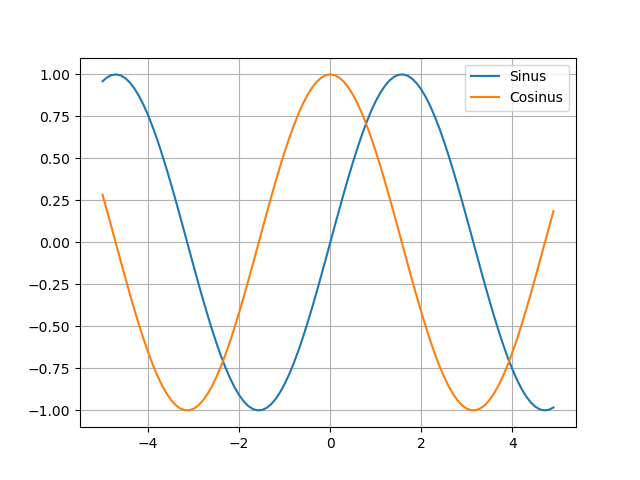
\includegraphics[width=\linewidth]{./gfx/plt-grid}
	\captionof{figure}{Plot mit Gitterlinien}
\end{tcolorbox}

\subsection{Titel und Achsenbeschriftung hinzufügen -- \texttt{title}, \texttt{xlabel}, \texttt{ylabel}}
Neben einer Legende sollten bei Plots auch Titel und Achsenbeschreibungen nicht fehlen. Diese lassen sich einfach über die Befehle \texttt{title}, \texttt{xlabel} und \texttt{ylabel} hinzugefügt werden. Das folgende Beispiel illustriert dies anhand der \emph{spektralen Strahlungsdichte eines idealen schwarzen Körpers}
\footnote{Crash-Kurs Physik:\\
Jeder Körper strahlt elektromagnetische Strahlung aus -- in einfachen Worten, jeder Körper leuchtet. Die Intensität und Lichtfarbe sind von der Temperatur abhängig. Heiße Körper glühen daher rot, sehr heiße Körper kommen sogar bis zur Weißglut; bei \enquote{kühlen} \SI{37}{\celsius} \enquote{leuchten} wir Menschen nur im Infrarot-Bereich. Aus diesem Grund sehen wir zwar nicht immer die Strahlung, die von jedem Körper ausgestrahlt wird, können diese aber trotzdem messen. Das gezeigte Programm berechnet die Intensität der einzelnen Licht-Wellenlängen, die ein Körper mit einer gegebenen Temperatur \texttt{T} ausstrahlt.\\
Streng genommen spielt hierbei auch die Farbe des Körpers eine Rolle; daher sprechen PhysikerInnen auch von \emph{Schwarzkörperstrahlung}. In der Praxis ist dieser Zusammenhang oft vernachlässigbar. Sekunden-Thermometer und Wärmebildkameras funktionieren nach diesem Prinzip: Ein Bild im Infraroten wird vom Objekt aufgenommen; die \enquote{Farbe} der gemessenen Strahlung wird dann als Temperatur interpretiert. Im gezeigten Plot liegt das Strahlungs-Maximum bei ca. \SI{20}{THz}, was einer Wellenlänge von \SI{15}{\micro\meter} entspricht -- weit außerhalb des Rahmens menschlicher Wahrnehmung, die zwischen ca. 400 und \SI{800}{\nano\meter} stattfindet, und damit in Übereinstimmung mit der täglichen Wahrnehmung, dass wir unsere Mitmenschen nicht glühen sehen.\\
Wenn Sie in Zeile 5 den Wert für \texttt{T} auf \inPy{5700} ändern und in Zeile 12 den Plot-Bereich auf \inPy{1e+15} erweitern, wird Ihnen das Spektrum der Sonne mit Maximum im sichtbaren Licht dargestellt.}:

\begin{codebox}[Beispiel: Plot mit Titel und Labels]
\begin{minted}[linenos]{python3}
import math
import matplotlib.pyplot as plt

h  = 6.62607015e-34     # Planck constant
T  = 300                # temperature in Kelvin
c  = 299792458          # speed of light
kB = 1.380649e-23       # Boltzmann constant

spectralDensity = lambda nu : ((2 * h * nu**3) / (c**2))  / \
                              (math.exp((h * nu) / (kB * T)) - 1)
\end{minted}
\end{codebox}
%
\begin{codebox}[]
\begin{minted}[linenos, firstnumber=last]{python3}
X = [x for x in range(1, int(1e+14), int(1e+10))]
Y = [spectralDensity(x) for x in X]

plt.title("Schwarzkörperstrahlung")
plt.xlabel("Strahlungsfrequenz in Hz")
plt.ylabel("Intensität in W/m²")

plt.plot(X, Y)
plt.show()
\end{minted}
\end{codebox}
%
\begin{tcolorbox}[title=Ausgabe: Plot mit Titel und Labels]
	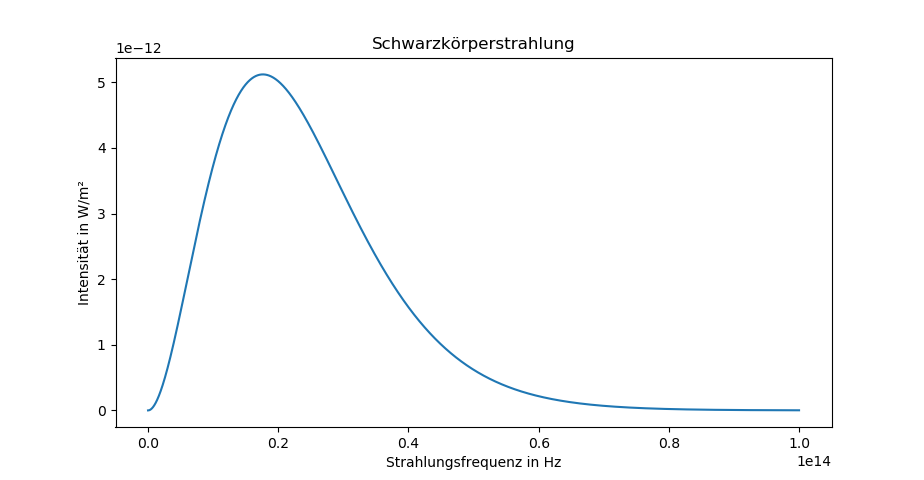
\includegraphics[width=\linewidth]{./gfx/plt-labels}
	\captionof{figure}{Plot mit Titel und Achsenbeschriftungen}
\end{tcolorbox}

\subsection{Skalierung der Achsen -- \texttt{xscale}, \texttt{yscale} und \texttt{xlim}, \texttt{ylim}}
Wenn Plots einen großen Wertebereich abdecken, kann es sinnvoll sein, die Werte \emph{logarithmisch} aufzutragen. Eine oder mehrere Achsen werden dabei verzerrt, um über mehrere Größenordnungen hinweg Änderungen gut zu verfolgen. Hierzu dienen die Befehle \texttt{xscale} und \texttt{yscale}.

\begin{codebox}[Beispiel: Linearer und Logarithmischer Plot]
\begin{minted}[linenos]{python3}
import matplotlib.pyplot as plt

W  = 500
X  = [x / 10 for x in range(-W, W)]
Y1 = [2 ** x for x in X]
Y2 = [x ** 7 for x in X]
\end{minted}
\end{codebox}
%
\begin{codebox}[]
\begin{minted}[linenos, firstnumber=last]{python3}
plt.title("Linear Plot")
plt.plot(X, Y1, label="exponential")
plt.plot(X, Y2, label="power")
plt.legend()
plt.show()

plt.title("Logarithmic Plot")
plt.yscale("log")
plt.plot(X, Y1, label="exponential")
plt.plot(X, Y2, label="power")
plt.legend()
plt.show()
\end{minted}
\end{codebox}

\begin{tcbraster}[raster columns=2,
                  raster equal height,
                  nobeforeafter,
                  raster column skip=0.5cm]
\begin{tcolorbox}[title=Lineare Auftragung]
	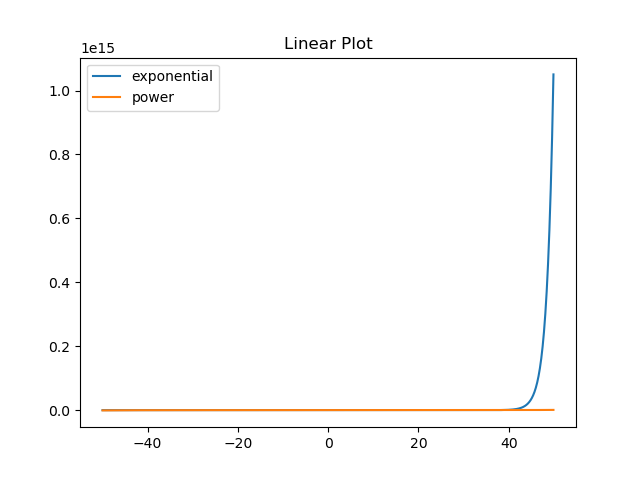
\includegraphics[width=\linewidth]{./gfx/plt-linear}
	\captionof{figure}{Linearer Plot}
	\label{gfx:PlotLinear}
\end{tcolorbox}
%
\begin{tcolorbox}[title=Logarithmische Auftragung]
	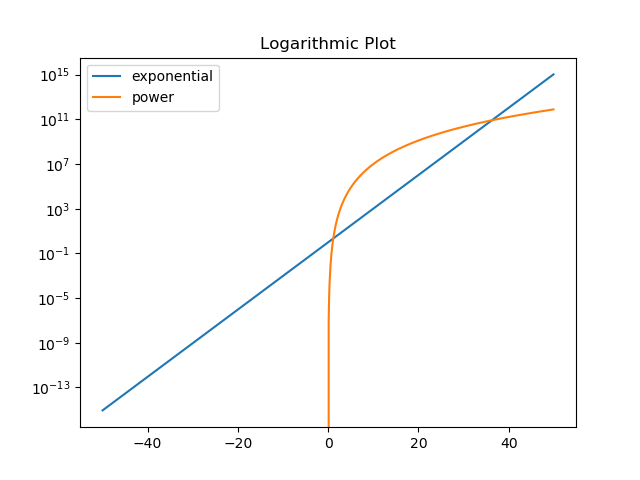
\includegraphics[width=\linewidth]{./gfx/plt-logarithmic}
	\captionof{figure}{Logarithmischer Plot}
	\label{gfx:PlotLogarithmic}
\end{tcolorbox}
\end{tcbraster}

In Abbildung \ref{gfx:PlotLinear} können wir kaum Details erkennen: Beide Plots bleiben \enquote{nahe} an der Null, bis die Exponentialfunktion irgendwann \enquote{explodiert}. Erst bei der logarithmischen Auftragung (Abbildung \ref{gfx:PlotLogarithmic}) sehen wir, dass das Polynom (orange Linie) zeitweise sogar größer ist als die Exponentialfunktion.

Wir haben diese Verzerrung erreicht, indem wir in Zeile 19 die y-Achse logarithmisch skaliert haben. Ebenso könnten wir mit \inPy{plt.xscale("log")} auch die x-Achse verzerren.

Der Logarithmus von 0 oder negativen Werten ist nicht definiert\footnote{liebe MathematikerInnen: natürlich beziehe ich mich auf den reellwertigen Logarithmus bzw. auf den Hauptzweig des Logarithmus.}. Um dennoch mit Werten umzugehen, die das Vorzeichen wechseln können und aber sinnvoller logarithmisch aufgetragen werden sollten, existiert auch die Option \inPy{"symlog"}. Hier wird jeweils der Logarithmus \emph{des Betrags} der Werte aufgetragen; abhängig vom Vorzeichen geschieht dies dann nach oben oder unten (\inPy{plt.yscale("simlog")} bzw. nach links oder rechts (\inPy{plt.xscale("simlog")}. Werte nahe der 0 werden linear aufgetragen. Was als nahe der 0 gelten soll, kann mit den Keyword-Arguments \texttt{linthreshx} bzw. \texttt{linthreshy} bestimmt werden. Die Grenzen des linearen bereichs sind auch als Hilfslinien sichtbar, wenn \texttt{grid} benutzt wird.

Für statistische Auswertungen ist manchmal auch der \enquote{Logit} einer Wahrscheinlichkeit interessant ($\text{logit}(y) = \log(\frac{y}{1-y})$). Für y-Werte zwischen 0 und 1 kann so auch \inPy{plt.xscale("logit")} eingestellt werden.

\begin{codebox}[Beispiel: Auftragung mit \texttt{symlog}]
\begin{minted}[linenos]{python3}
import math
import matplotlib.pyplot as plt

W  = 500
X  = [x / 10 for x in range(-W, W)]
Y1 = [math.sin(x) for x in X]
Y2 = [x / 10      for x in X]

plt.xscale("symlog")
plt.plot(X, Y1)
plt.plot(X, Y2)
plt.grid()
plt.show()

plt.xscale("symlog", linthreshx=10)
plt.plot(X, Y1)
plt.plot(X, Y2)
plt.grid()
plt.show()
\end{minted}
\end{codebox}

\begin{tcolorbox}[title=Auftragung mit \texttt{symlog}]
	\begin{minipage}{.49\linewidth}
		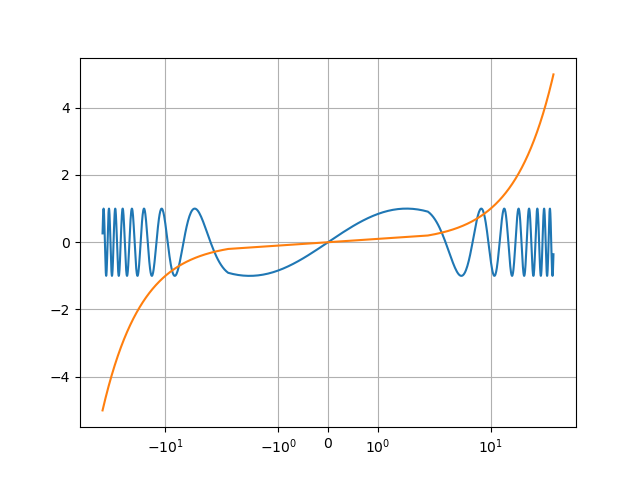
\includegraphics[width=\linewidth]{./gfx/plt-symlog}
		\captionof{figure}{symmetrisch-logarithmische Auftragung mit Standard-Schranke für lineare Auftragung}
		\label{gfx:PlotSymlog}
	\end{minipage}
%
	\begin{minipage}{.49\linewidth}
		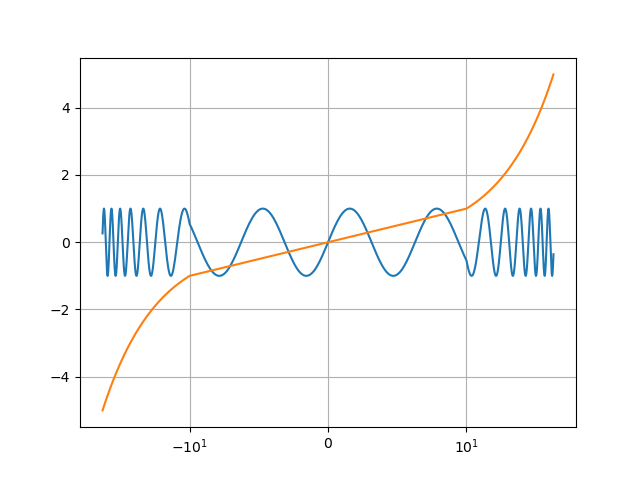
\includegraphics[width=\linewidth]{./gfx/plt-symlog-threshold}
		\captionof{figure}{symmetrisch-logarithmische Auftragung mit höherer Schranke für lineare Auftragung}
		\label{gfx:PlotSymlog-Threshold}
	\end{minipage}
\end{tcolorbox}

In Ähnlicher Manier kann mit \texttt{xlim} und \texttt{ylim} festgelegt werden, in welchen Grenzen die X- und Y-Achse skaliert werden sollen, unabhängig von den \enquote{Ausmaßen} des tatsächlichen Graphen. Der Graph füllt dann nicht mehr die gesamte Plot-Fläche aus, bzw. wird gegebenenfalls abgeschnitten:

\begin{codebox}[Beispiel: Manuell gewählte Plot-Skalierung, width=.55\linewidth, nobeforeafter, equal height group = grpXmpSimplePlotScale]
\begin{minted}[linenos]{python3}
import math
import matplotlib.pyplot as plt

N = 100
X = [(x - N/2) / 10 for x in range(N)]
Y = [math.sin(x) for x in X]

plt.plot(X, Y)
plt.xlim(-6  , +6)
plt.ylim(-0.7, +3)
plt.grid()
plt.show()
\end{minted}
\end{codebox}
%
\begin{tcolorbox}[title=Manuell gewählte Plot-Skalierung, width=.45\linewidth, nobeforeafter, equal height group = grpXmpSimplePlotScale]
	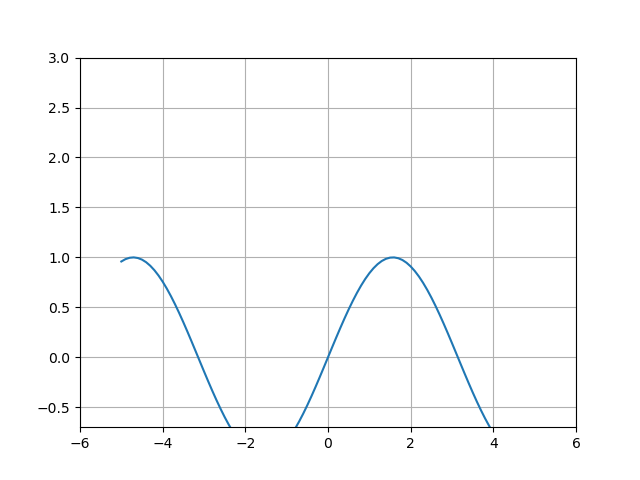
\includegraphics[width=\linewidth]{./gfx/plt-limits}
	\captionof{figure}{Manuelle Skalierung}
\end{tcolorbox}

\subsection{Andere Plot-Arten}
Neben Kurven in einem X-Y-Diagramm kann die MatPlotLib auch andere Arten von Visualisierungen erzeugen.

\subsubsection{Barplots}
Barplots oder Balkendiagramme verhalten sich ähnlich wie die Punkt- oder Liniendiagramme, die im letzten Abschnitt gezeigt wurden. Alle oben erwähnten Befehle funktionieren auch hier, außerdem kann auch das Keyword-Argument \texttt{color} verwendet werden. Erstellt werden Barplots mit den Befehlen \texttt{bar} (vertikale Balken) und \texttt{barh} (horizontale Balken). Die \enquote{X-Werte} dürfen für Barplots auch Strings enthalten, und werden entsprechend als Beschriftung angebracht.

\begin{codebox}[Beispiel: Barplots]
\begin{minted}[linenos]{python3}
import random
import matplotlib.pyplot as plt

X = ["Smoot", "Fnord", "R'lyeh"]
Y = [random.randint(0, 11) for x in X]   # this one goes up to eleven

plt.bar(X, Y, color="#0040B0FF")
plt.ylim(0, 11)
plt.show()

plt.barh(X, Y, color="#0040B0FF")
plt.xlim(0, 11)
plt.show()
\end{minted}
\end{codebox}
%
\begin{tcbraster}[raster columns=2,
                  raster equal height,
                  nobeforeafter,
                  raster column skip=0.5cm]
\begin{tcolorbox}[title=Vertikaler Barplot]
	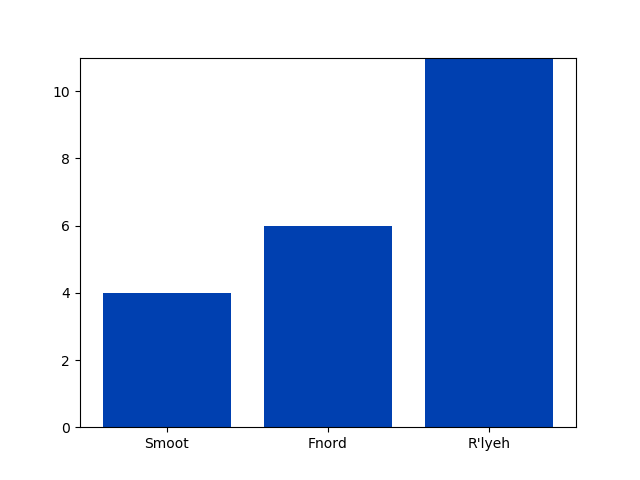
\includegraphics[width=\linewidth]{./gfx/plt-bars}
	\captionof{figure}{Vertikaler Barplot}
\end{tcolorbox}
%
\begin{tcolorbox}[title=Horizontaler Barplot]
	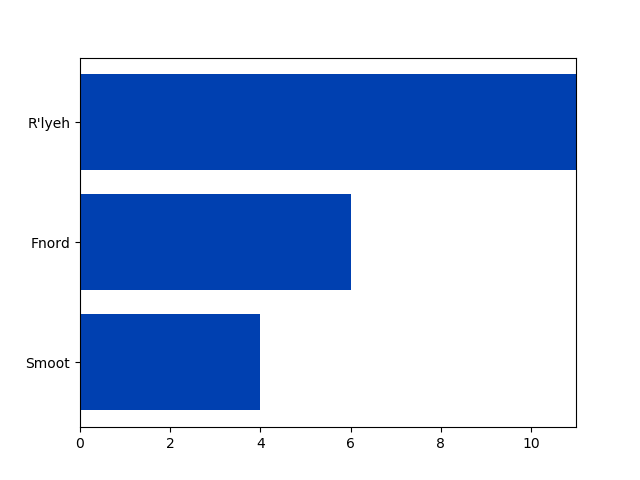
\includegraphics[width=\linewidth]{./gfx/plt-barh}
	\captionof{figure}{Horizontaler Barplot}
\end{tcolorbox}
\end{tcbraster}

\subsubsection{Kuchendiagramme}
pie
\subsubsection{Histogramme}
hist(data, bins, orientation='horizontal')
\subsubsection{Stackplots}
stackplot
\subsubsection{Scatterplots}
scatter
\subsubsection{Flussdiagramme}
quiver
\subsubsection{Äquipotentiallinien}
isosurface

\subsubsection{Weitere Diagrammtypen}
Unter \url{https://matplotlib.org/3.1.0/gallery/index.html} sind diverse Beispiele zum Umgang mit der MatPlotLib aufgeführt.


\section{Multiplots}
subplots

\section{Plot-Objekte}

\section{Ausgabe in Dateien}





%https://matplotlib.org/api/pyplot_api.html


save files, hintbox on data usage
	\chapter{Numpy}
\label{chp:Numpy}
%	\chapter{SciPy}


https://docs.scipy.org/doc/scipy/reference/tutorial/
https://xkcd.com/2048/
	
	\appendix
\begin{appendices}
\chapter{Begriffe}

\chapter{Tabellen}
%\section{Spezielle Rückgabewerte} \label{sec:specialRetVals}
\section{Magic Keywords (Dunders)}
\url{https://rszalski.github.io/magicmethods/}
\url{https://docs.python.org/3/reference/datamodel.html}

\end{appendices}

	
	\listoffigures
	\listoftables	
\end{document}